\documentclass[table,fleqn]{beamer}[10]
\usepackage{pgf}
%\usepackage[danish]{babel}
\usepackage[utf8]{inputenc}
\usepackage{beamerthemesplit}
\usepackage{graphics,epsfig, subfigure}
\usepackage{url}
\usepackage{srcltx}
\usepackage{hyperref}
\usepackage{multirow}
\usepackage{graphicx}
\usepackage{amsmath}
\usepackage{amsfonts}
\usepackage{multirow}
\usepackage{makecell}

\definecolor{kugreen}{RGB}{50,93,61}
\definecolor{kugreenlys}{RGB}{132,158,139}
\definecolor{kugreenlyslys}{RGB}{173,190,177}
\definecolor{kugreenlyslyslys}{RGB}{214,223,216}

\definecolor{lightblue}{RGB}{133, 192, 206}
\definecolor{darkblue}{RGB}{50, 70, 150}
\definecolor{grey}{RGB}{153, 153, 153}
\definecolor{red}{RGB}{255, 0, 0}

\newcommand{\semitransp}[2][35]{\color{fg!#1}#2}

\setbeamercovered{transparent}
\mode<presentation>
\usetheme[numbers,totalnumber,compress,sidebarshades]{PaloAlto}
\setbeamertemplate{footline}[frame number]

  \usecolortheme[named=kugreen]{structure}
  \useinnertheme{circles}
  \usefonttheme[onlymath]{serif}
  \setbeamercovered{transparent}
  \setbeamertemplate{blocks}[rounded][shadow=true]
  \useoutertheme{infolines} 
  
  \makeatletter
  \setbeamertemplate{sidebar \beamer@sidebarside}%{sidebar theme}
  {
    \beamer@tempdim=\beamer@sidebarwidth%
    \advance\beamer@tempdim by -6pt%
    \insertverticalnavigation{\beamer@sidebarwidth}%
    \vfill
    \ifx\beamer@sidebarside\beamer@lefttext%
    \else%
      \usebeamercolor{normal text}%
      \llap{\usebeamertemplate***{navigation symbols}\hskip0.1cm}%
      \vskip2pt%
    \fi%
  }%
\makeatother

\makeatother
\setbeamertemplate{footline}
{
  \leavevmode%
  \hbox{%
  \begin{beamercolorbox}[wd=1.0\paperwidth,ht=2.25ex,dp=1ex,center]{title in head/foot}%
    \usebeamerfont{title in head/foot} \hspace*{3em}
    \insertframenumber{} / \inserttotalframenumber\hspace*{1ex}
  \end{beamercolorbox}}%
  \vskip0pt%
}
\makeatletter

\logo{\includegraphics[width=1.0cm]{Tlogo}}
\title{Simultaneous Neural Machine Translation}
\author{Ashkan Alinejad \\ \vspace{0.5cm} Supervisor: Anoop Sarkar}
\institute{Simon Fraser University}
\date{10 January 2018}



\begin{document}
\frame{\titlepage \vspace{-0.5cm}
}

\frame
{
\frametitle{Overview}
\tableofcontents%[pausesection]
}

%===================================================================================
\section[NMT]{Neural Machine Translation}

%\frame{
%\begin{center}
%\Huge Neural Machine Translation
%\end{center}
%}

\subsection[Encoder-Decoder]{ $\diamond$ RNN Encoder-Decoder}

\frame{
\textbf{What is NMT?}
\begin{itemize}
    \item The approach of solving the problem of machine translation using one huge Neural Network.
    \item the most common approach is encoder-decoder model.
\end{itemize}
}

%\frame{
%\textbf{Encoder-Decoder Structure}
%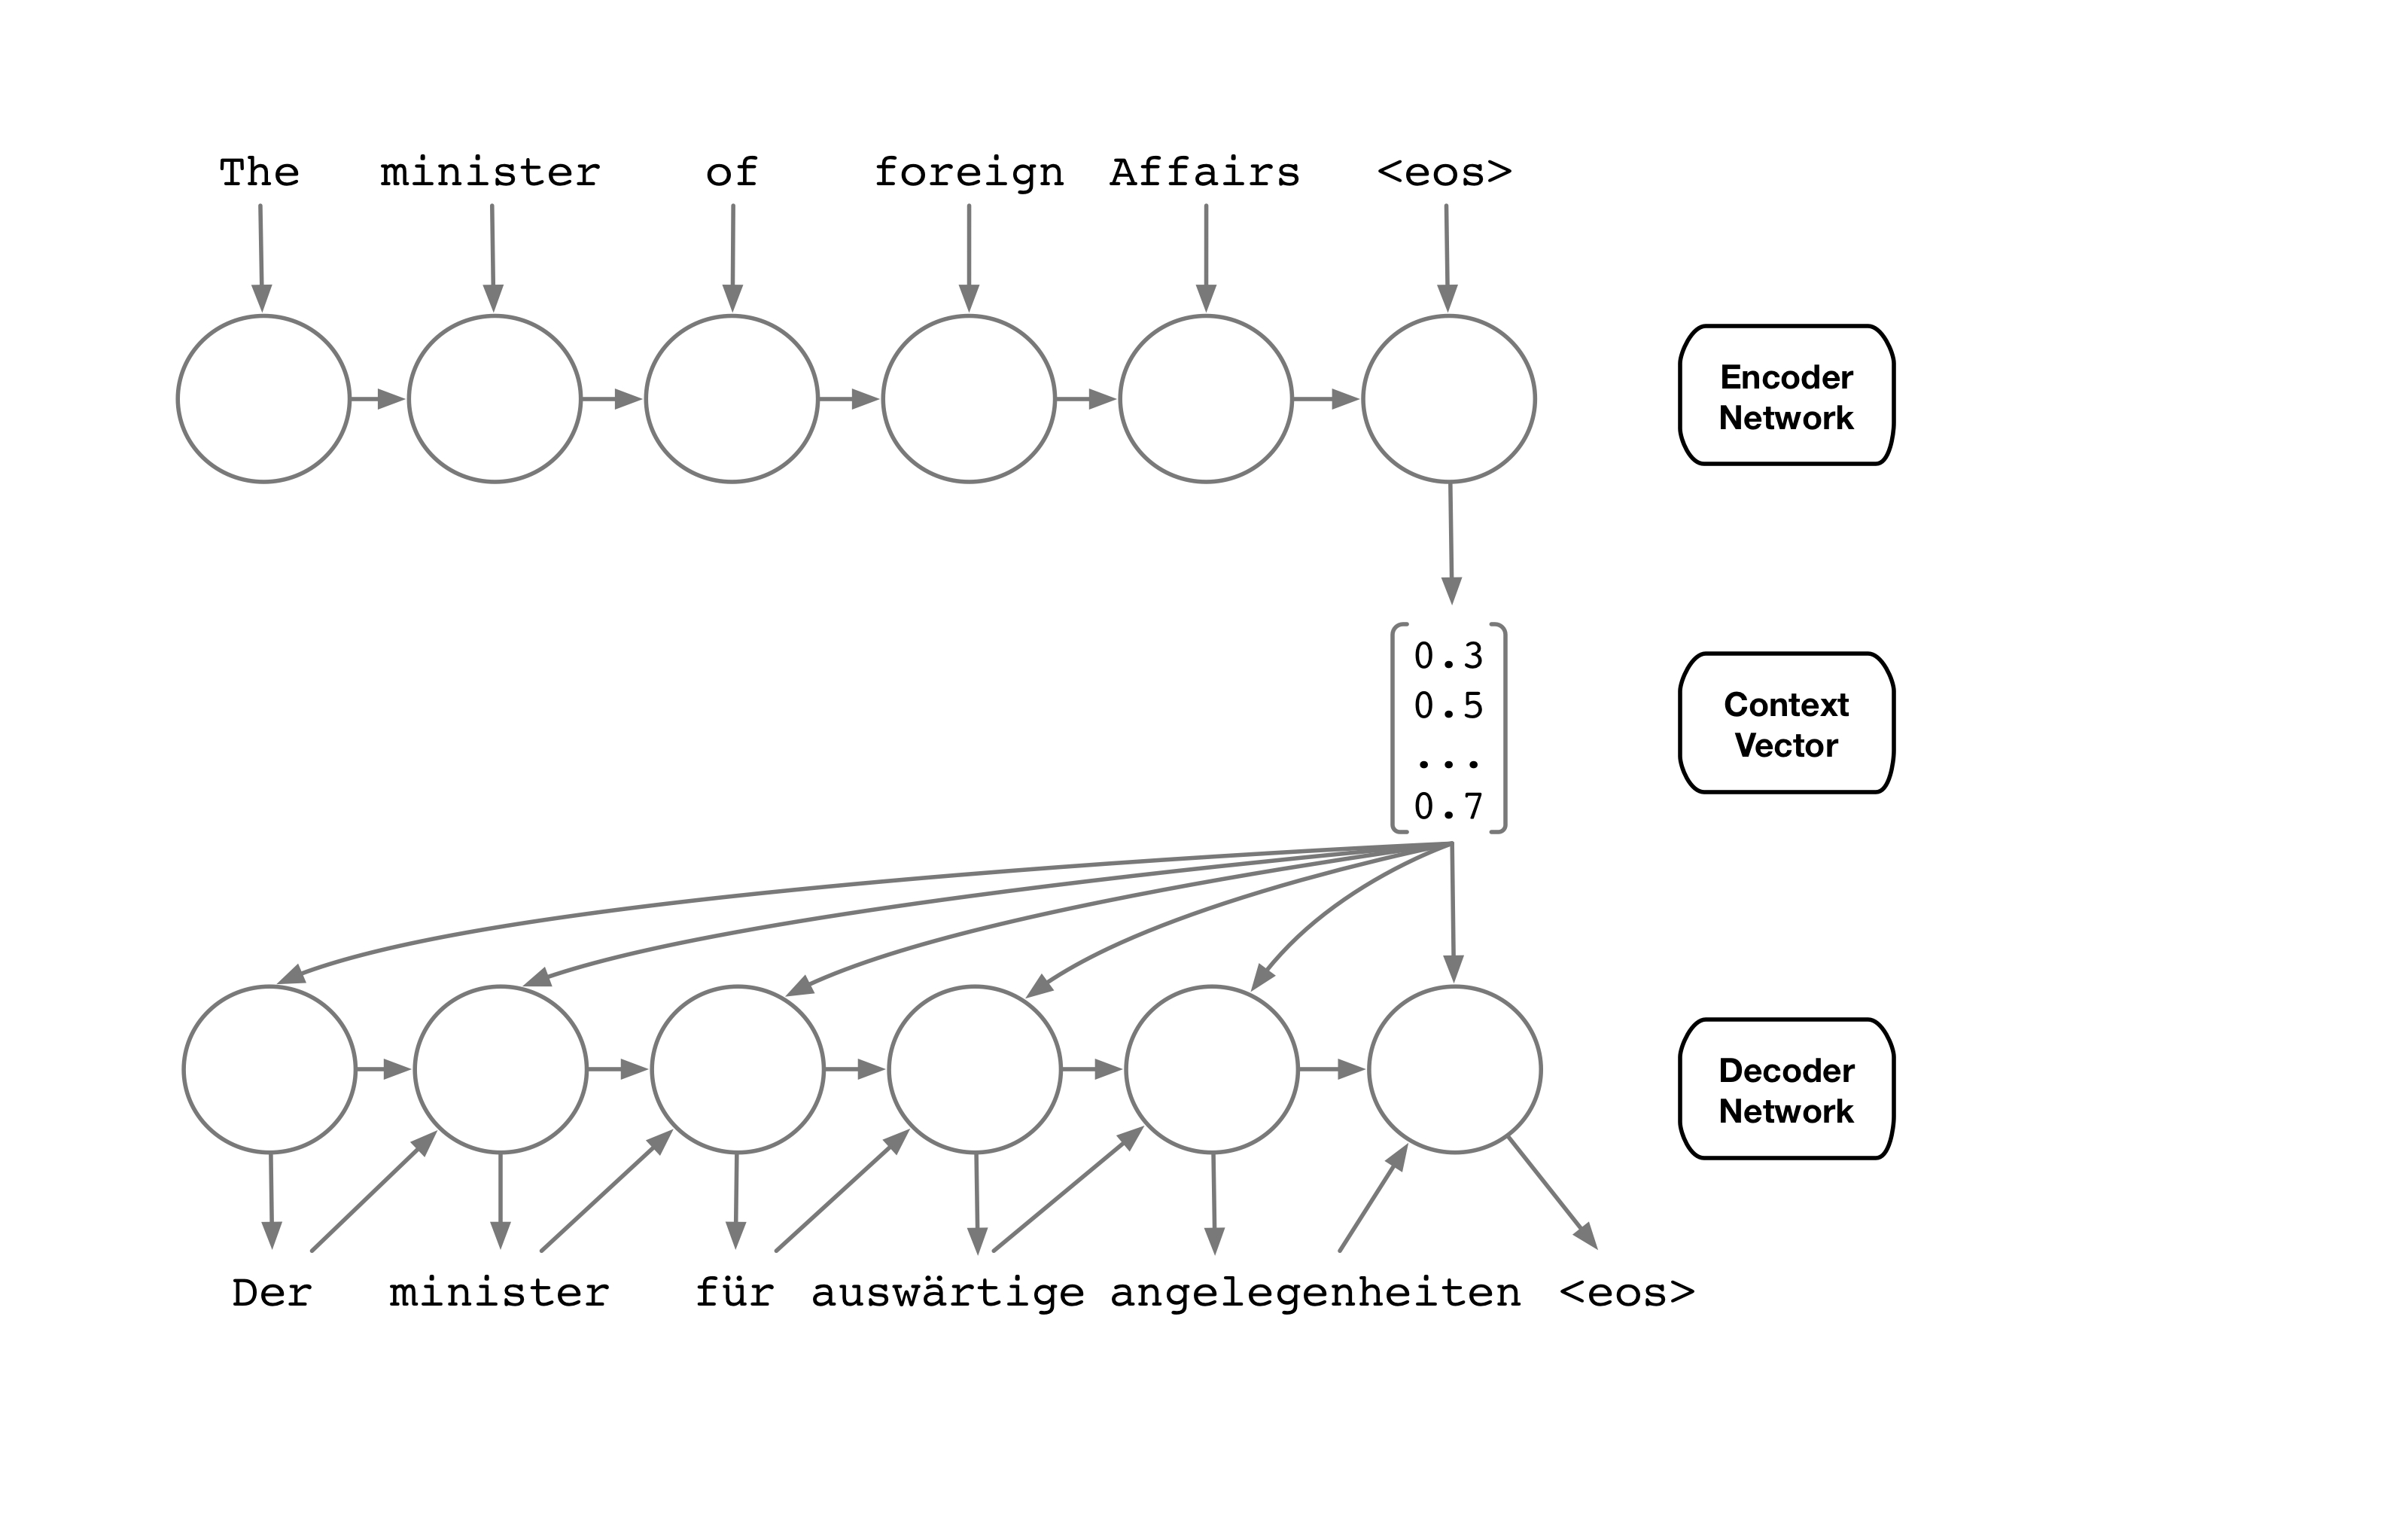
\includegraphics[scale=0.09]{./images/EncDec0}
%}

\frame{
\only<1>{
\textbf{Encoder-Decoder Structure}\\
\vspace{0.5cm}
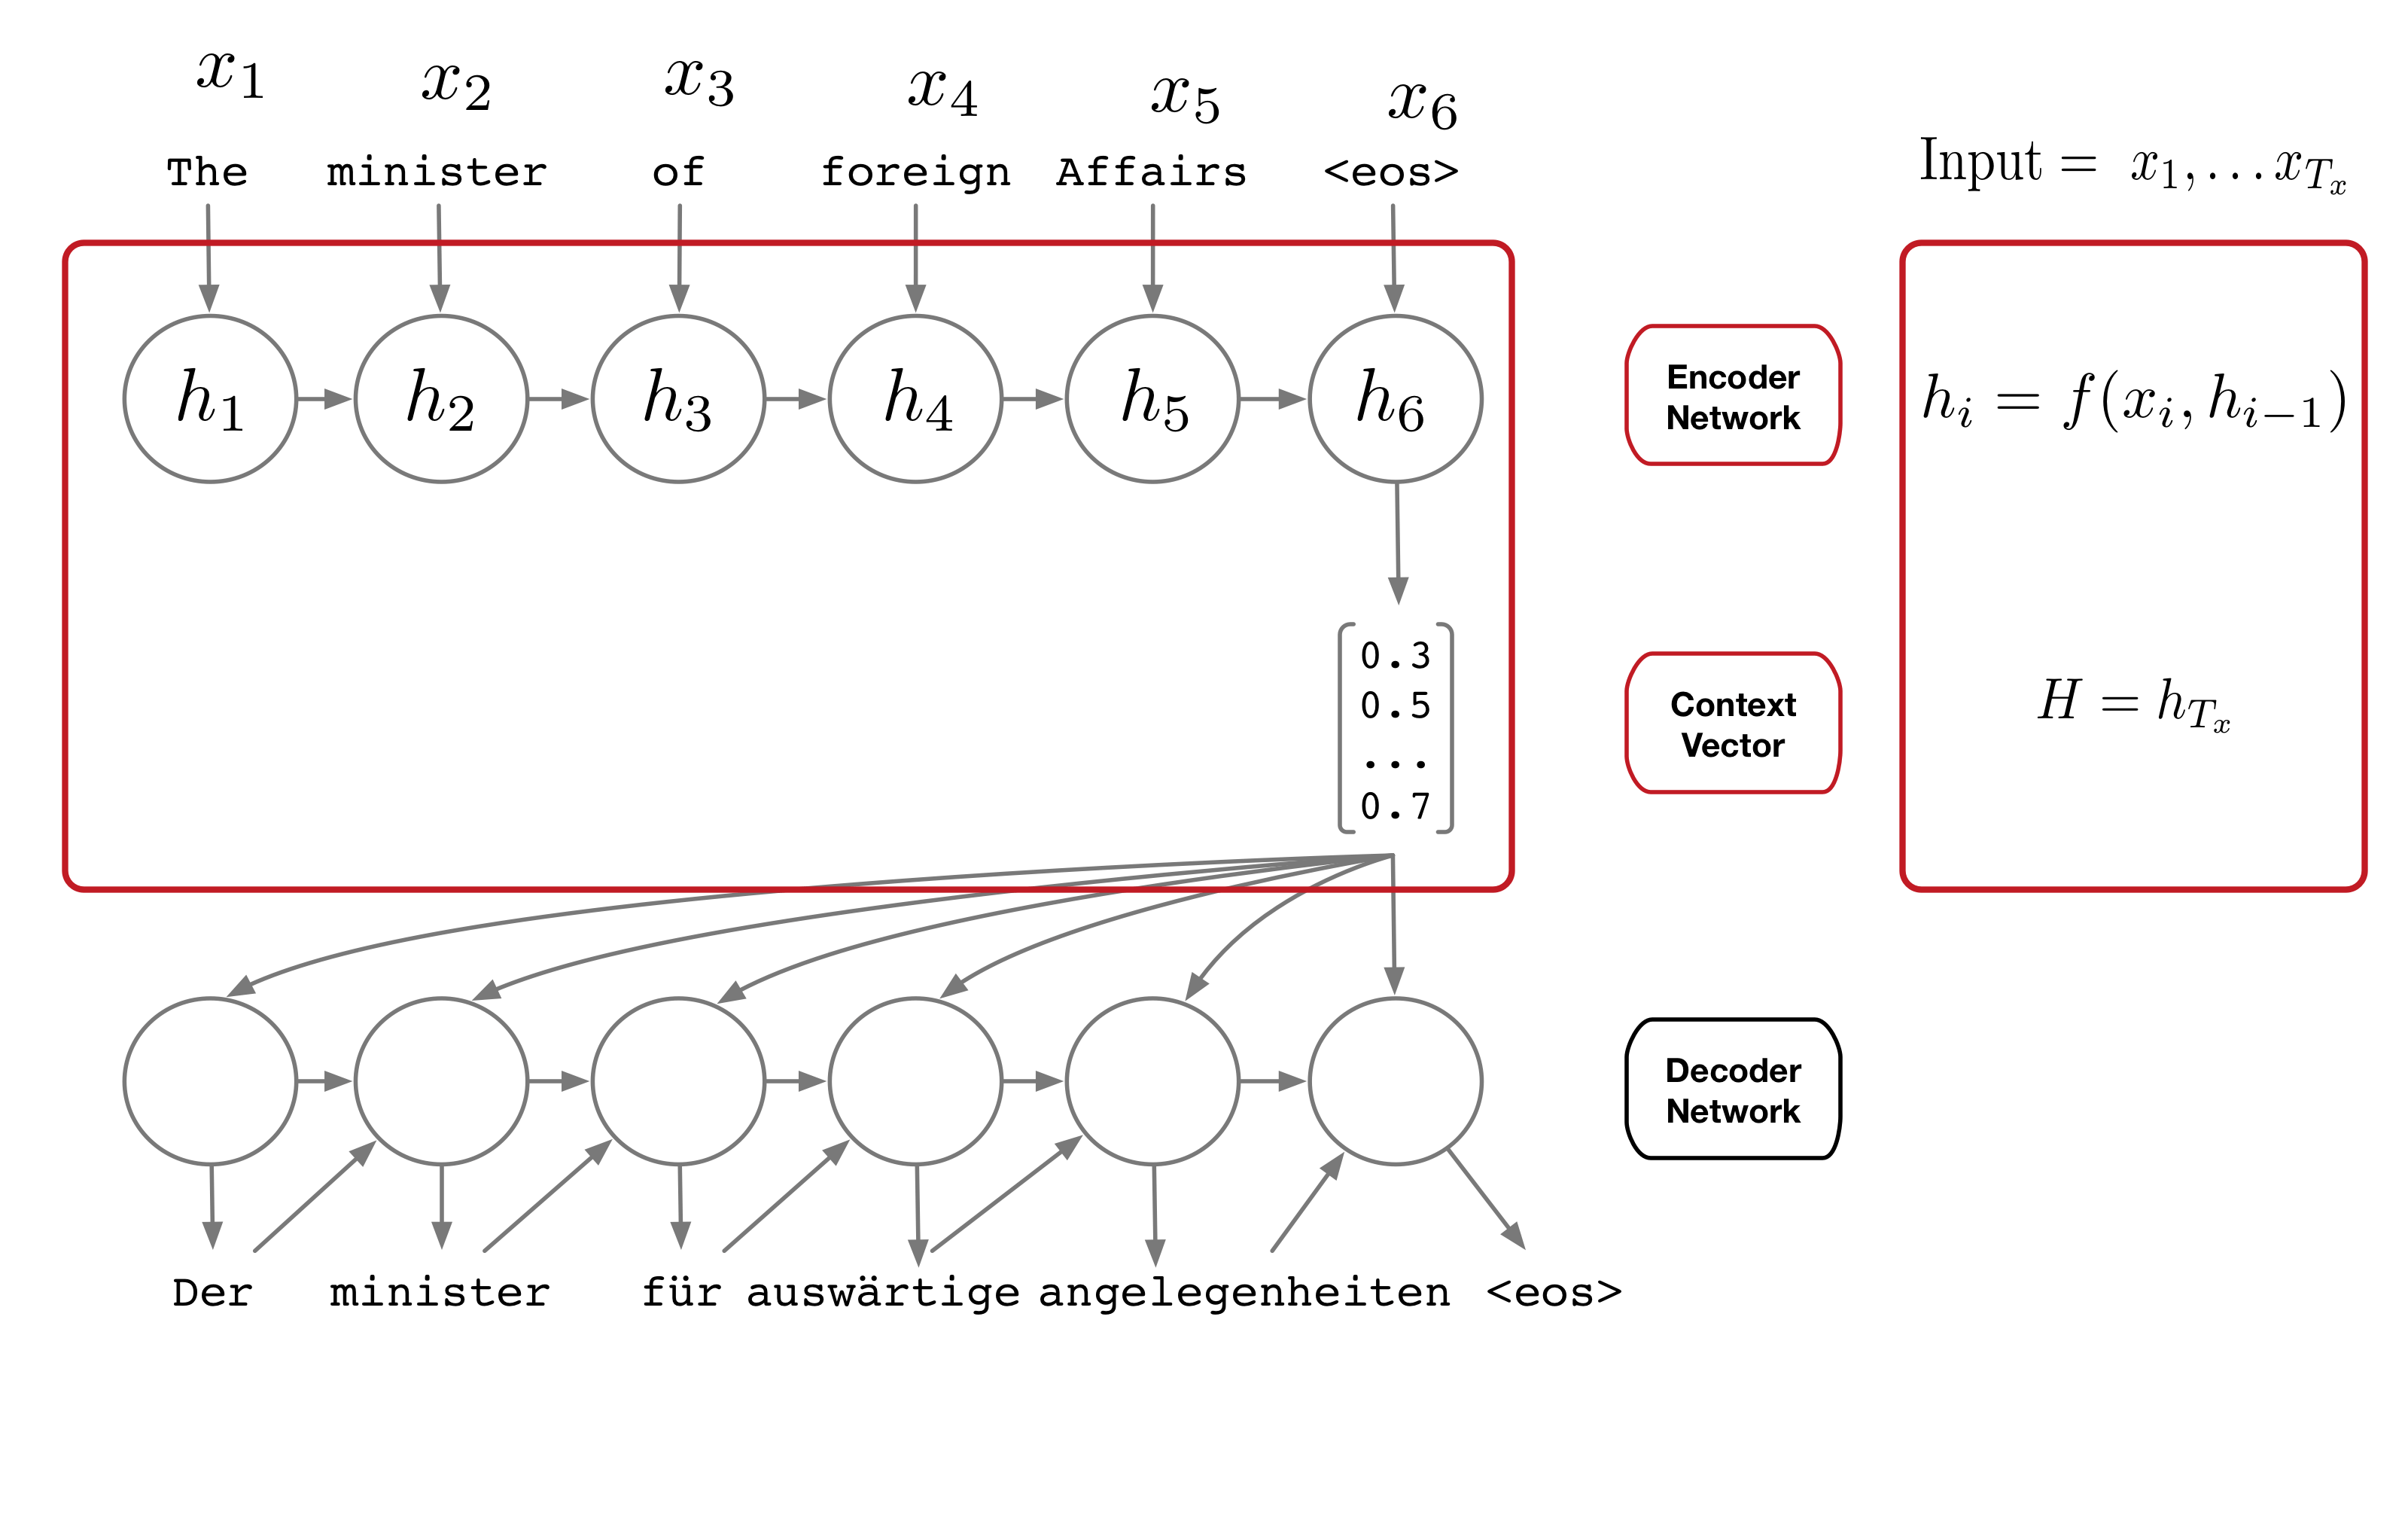
\includegraphics[scale=0.09]{./images/EncDec1}
}

\only<2>{
\textbf{Encoder-Decoder Structure}\\
\vspace{0.5cm}
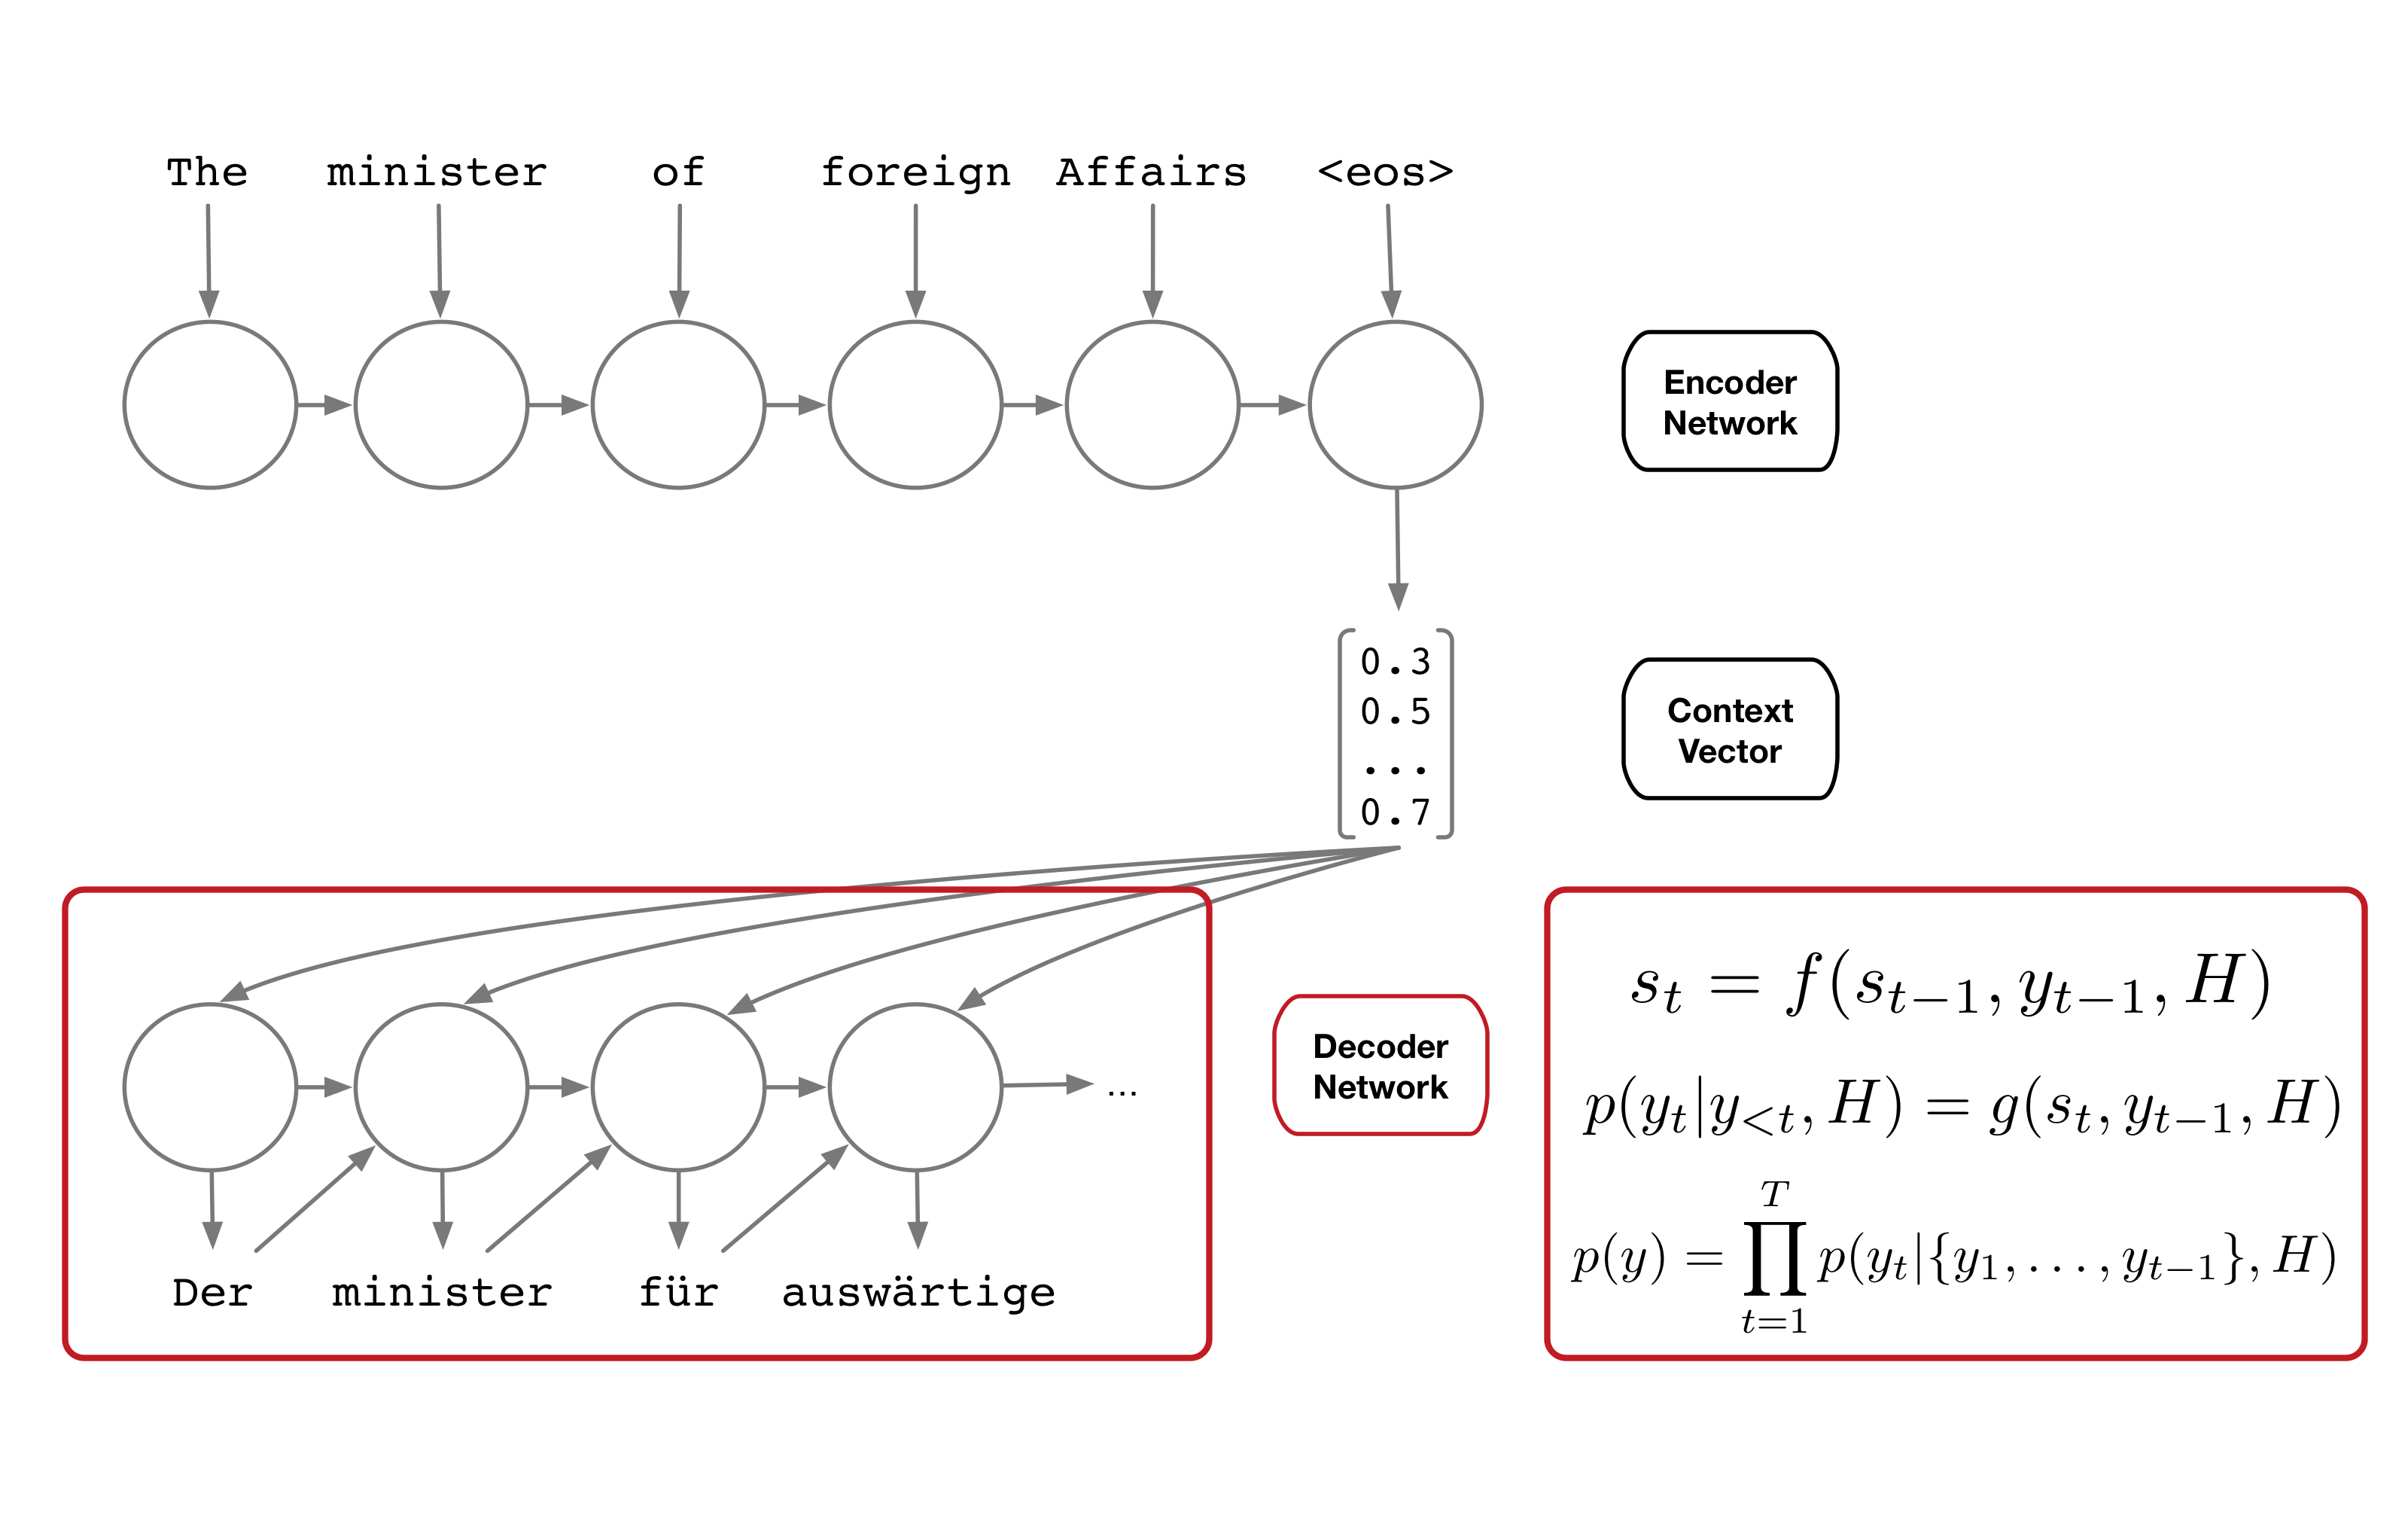
\includegraphics[scale=0.09]{./images/EncDec2}
}
}

\subsection[Attention]{ $\diamond$ Attention Mechanism}
\frame{
\textbf{Attention Mechanism}
\begin{itemize}
    \item We are conditioning over one fixed-dimensional context vector
    \item Works good on short sentences but not on the long ones.
    \item Attention mechanism tries to solve it.
\end{itemize}
}

\frame{
\textbf{Attention Mechanism}
\only<1>{
\begin{center}
    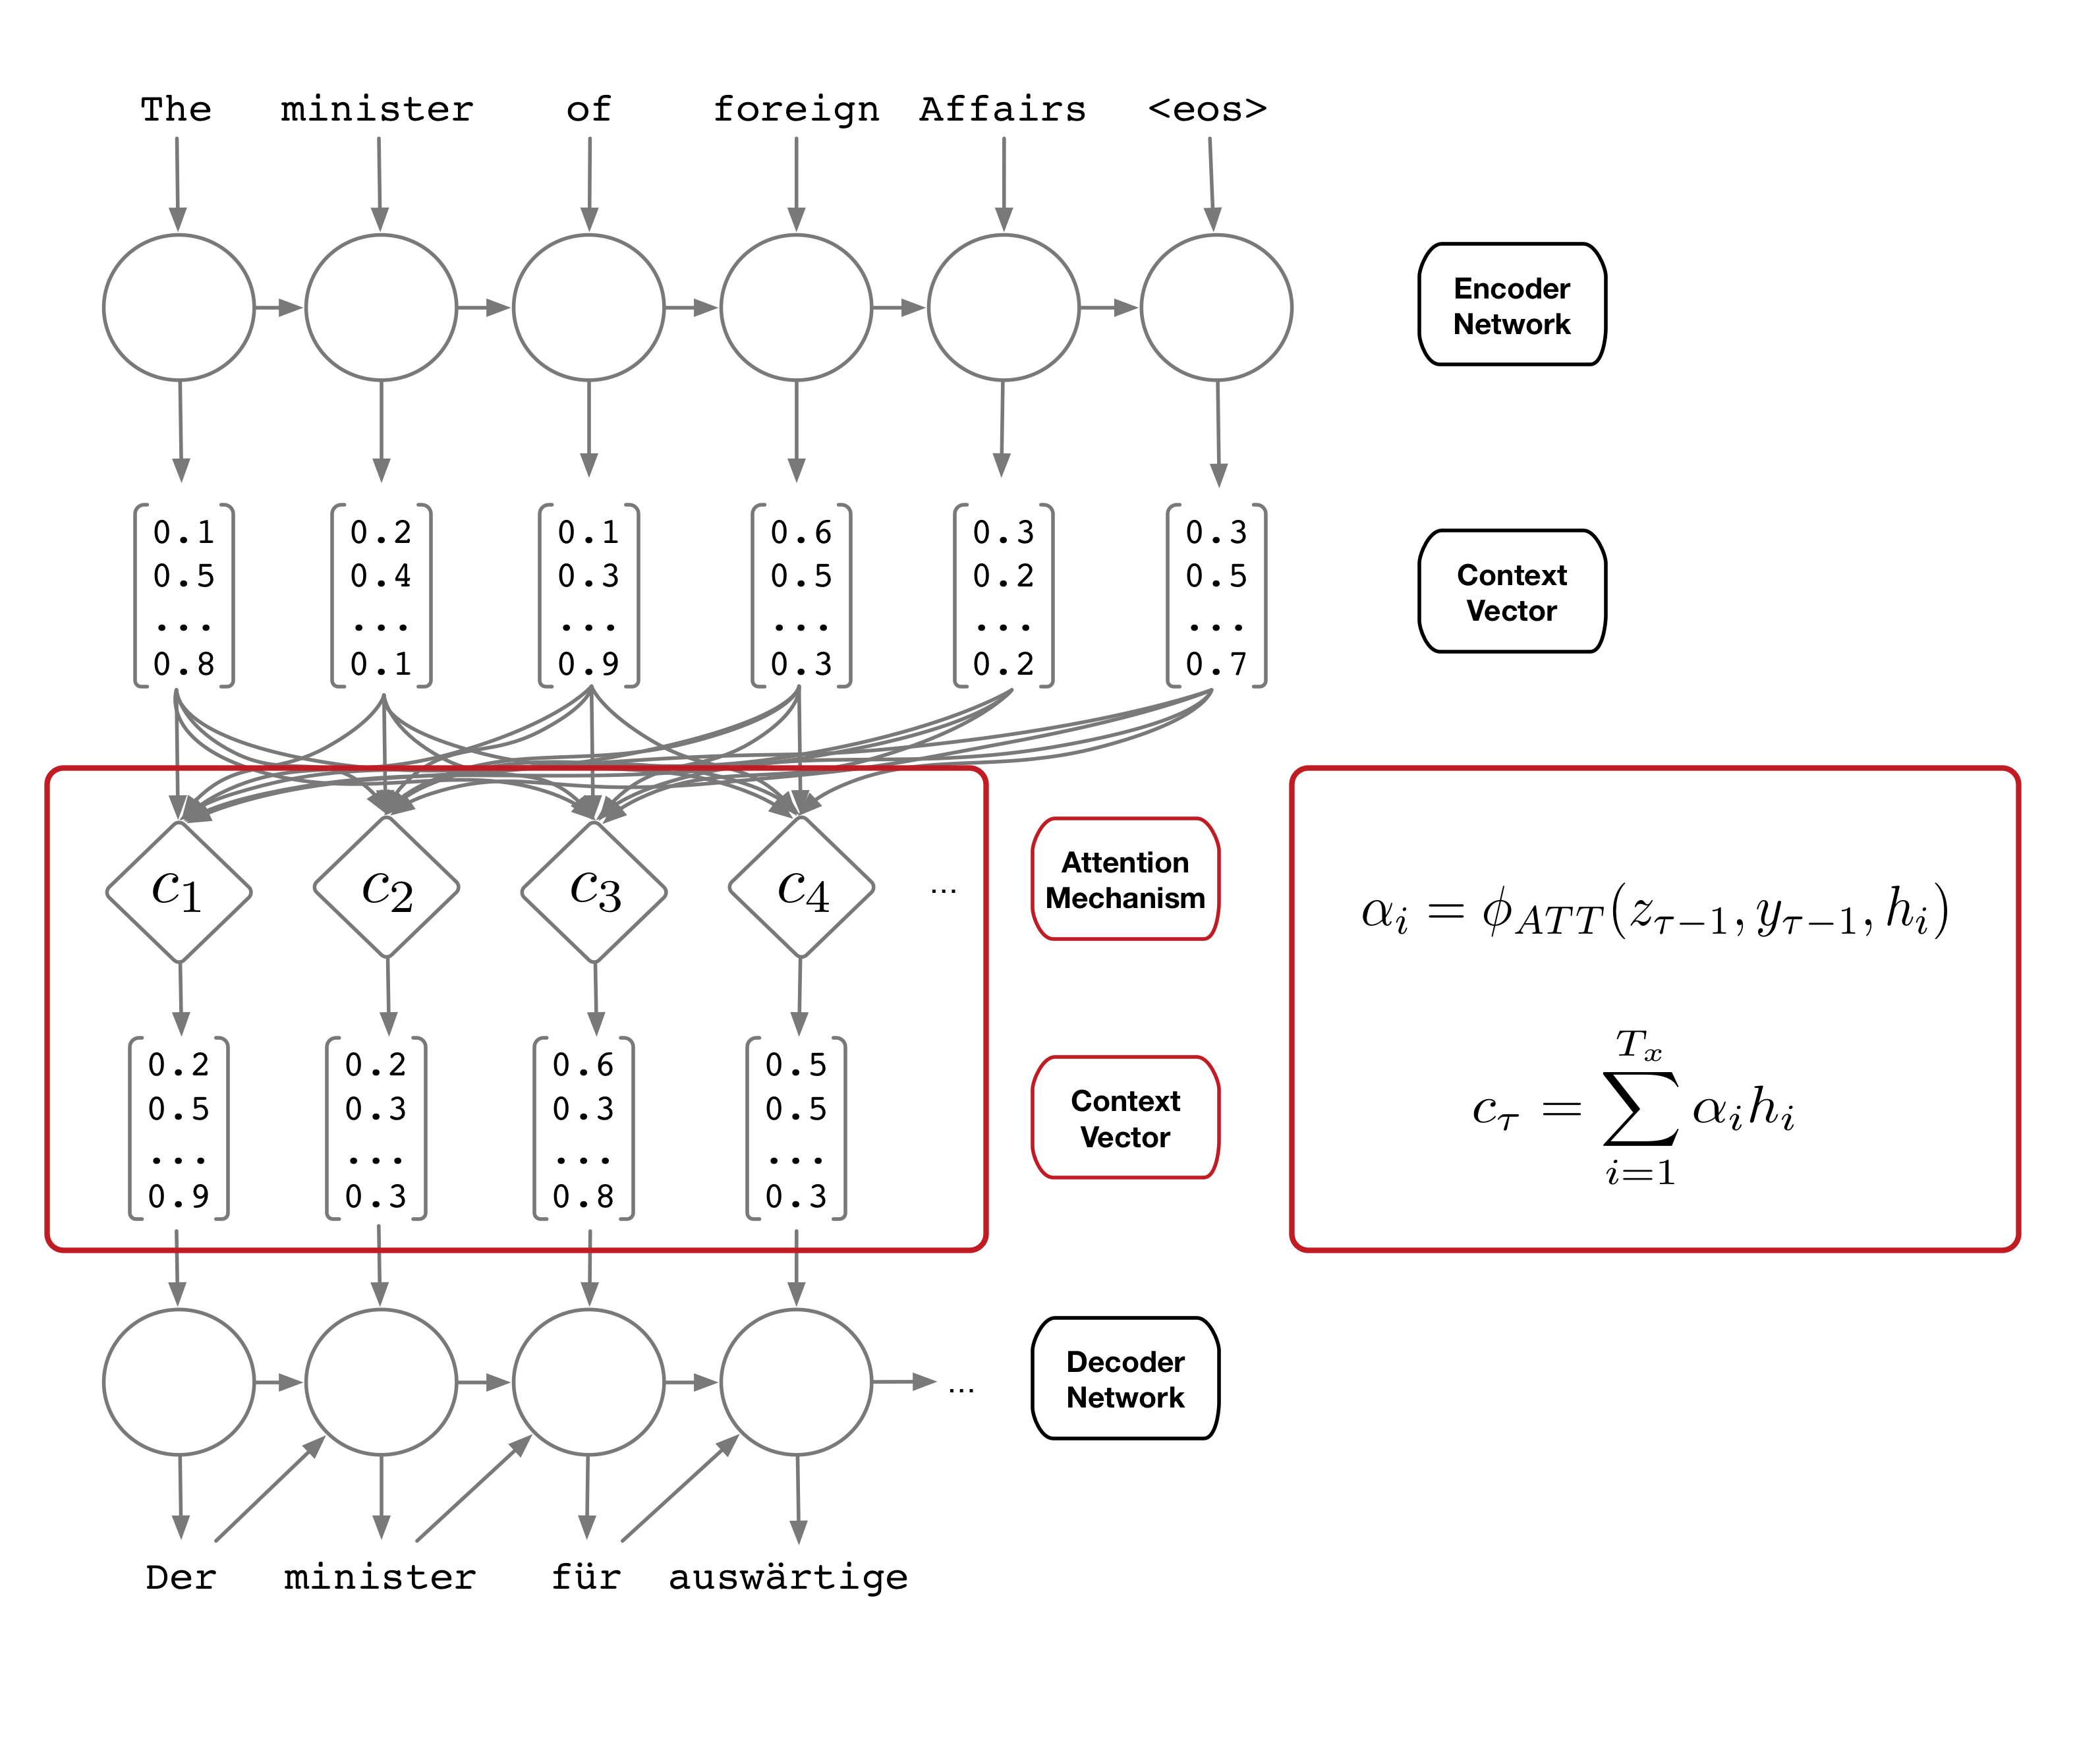
\includegraphics[scale=0.085]{./images/att1}
\end{center}
}
\only<2>{
\begin{center}
    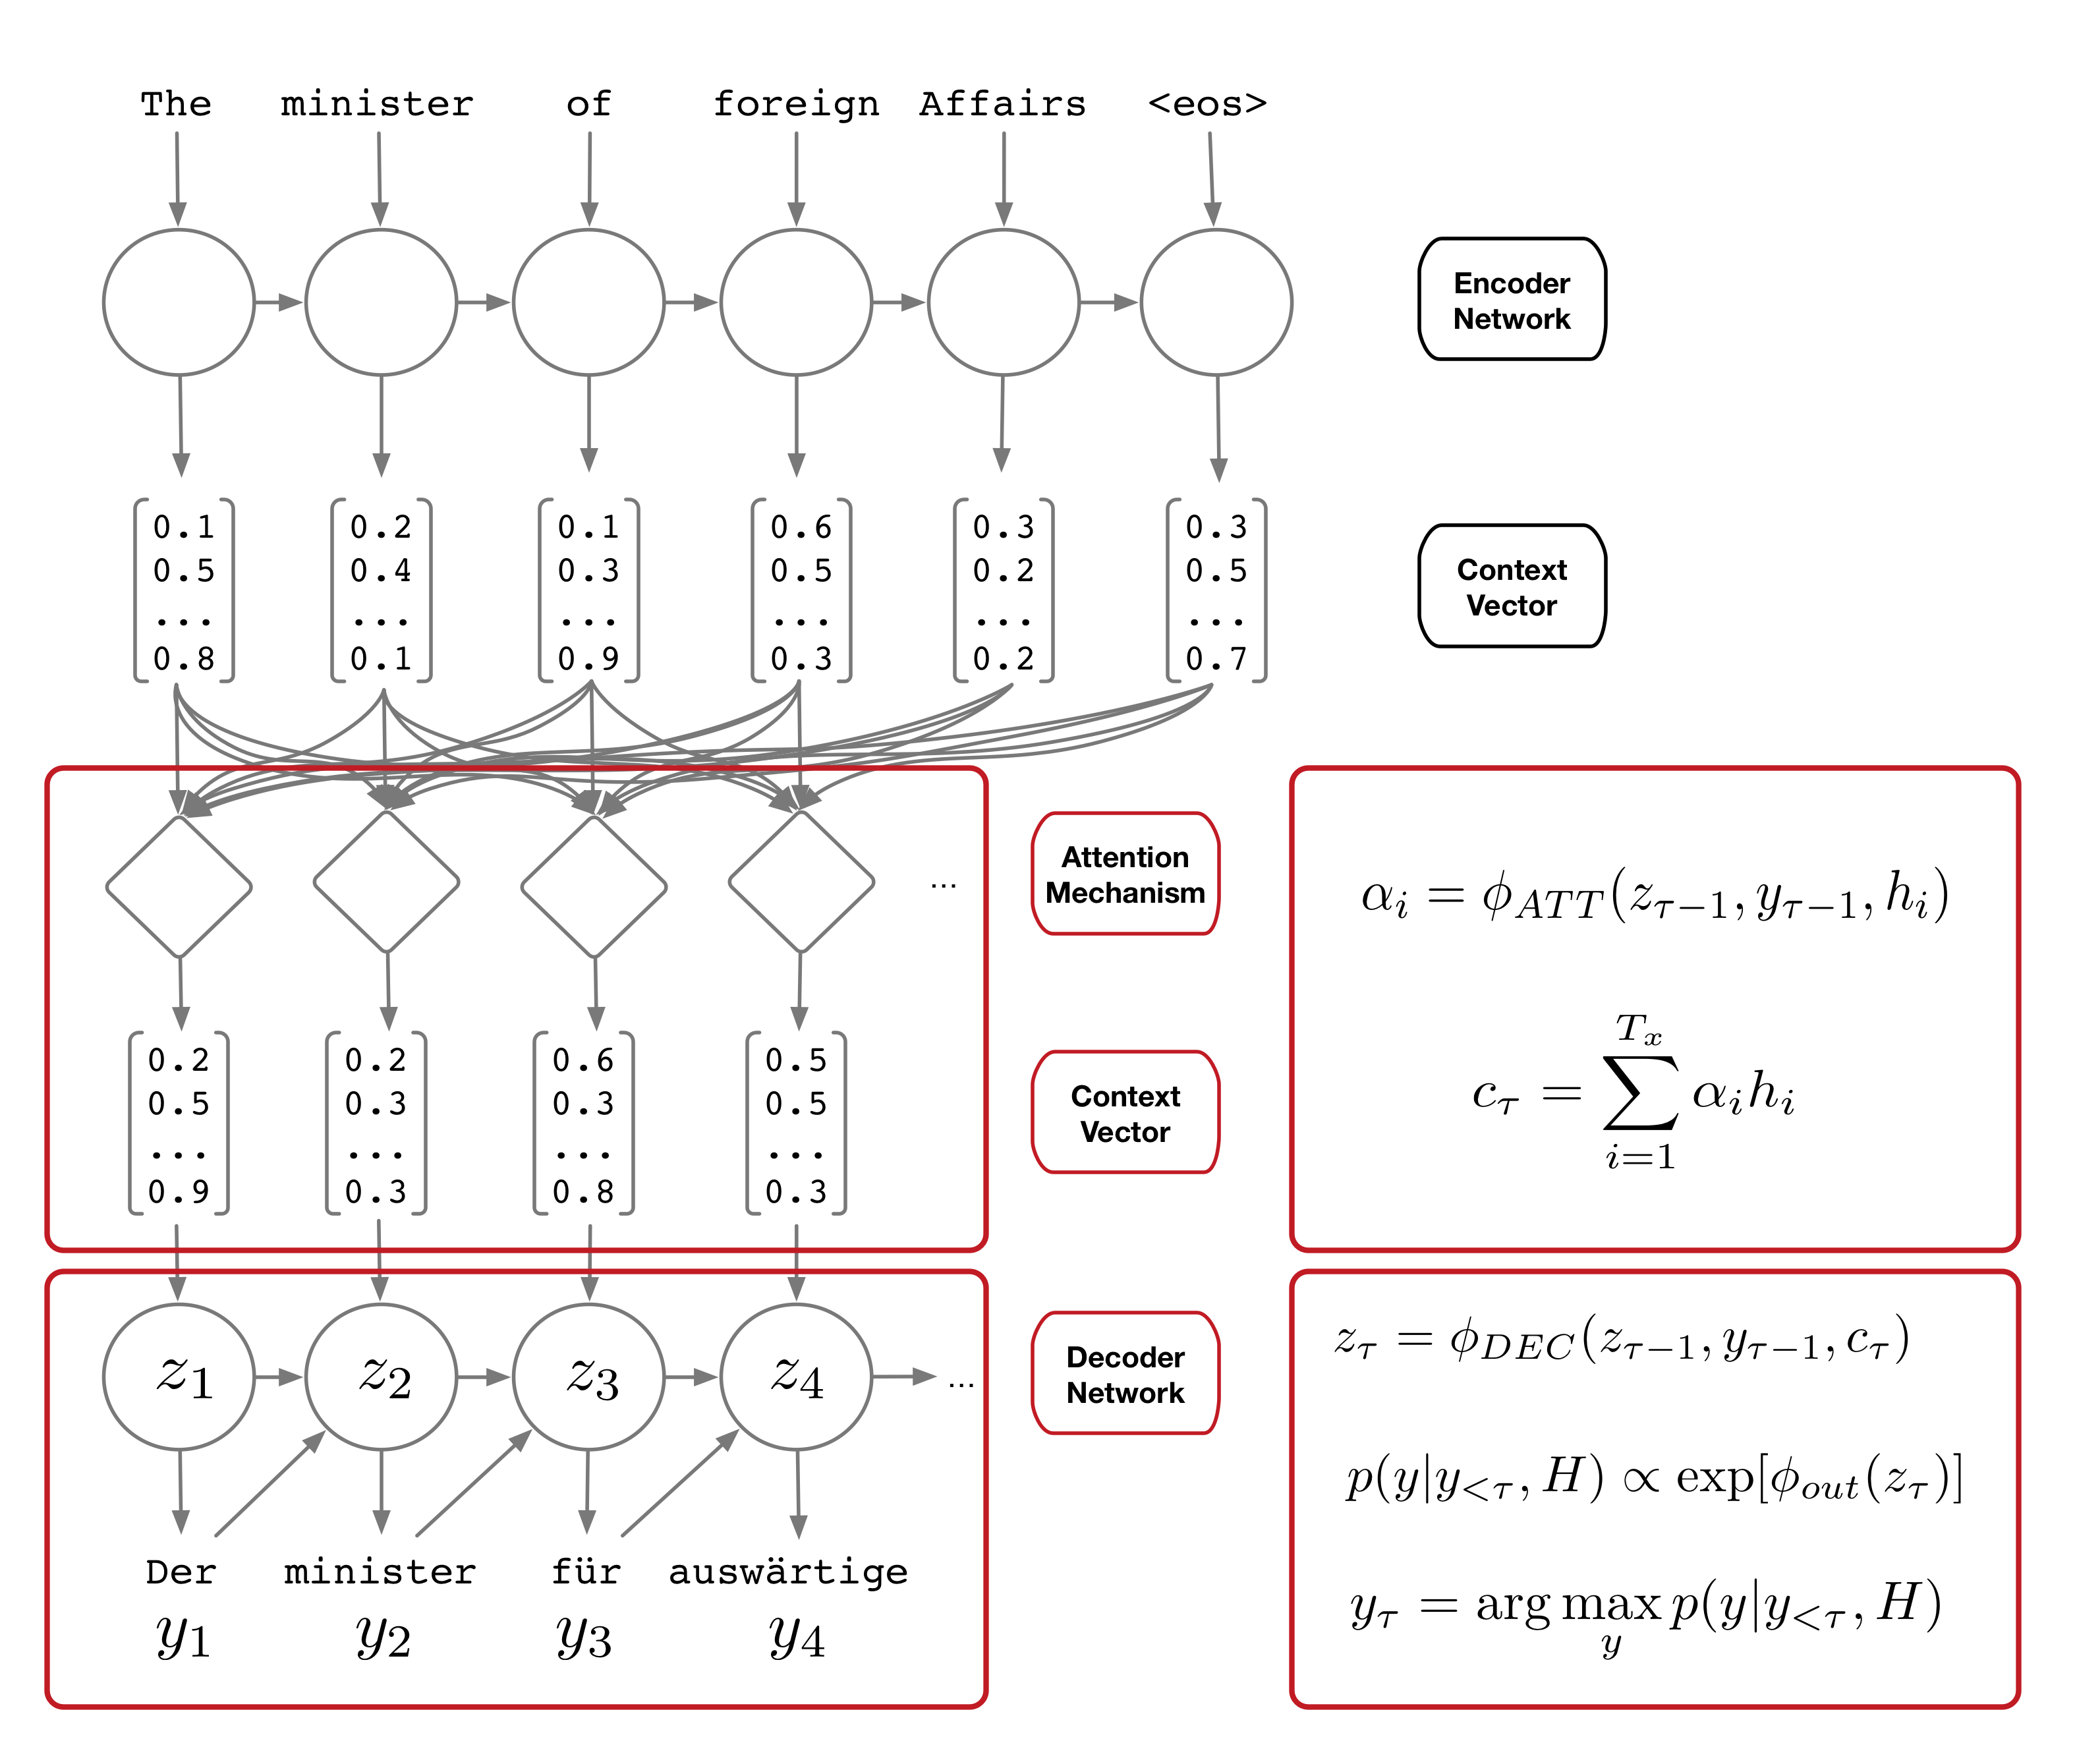
\includegraphics[scale=0.23]{./images/att2}
\end{center}
}
}

\frame{
\textbf{Attention Mechanism}
%\vspace{5mm}
\begin{figure}
    \centering
    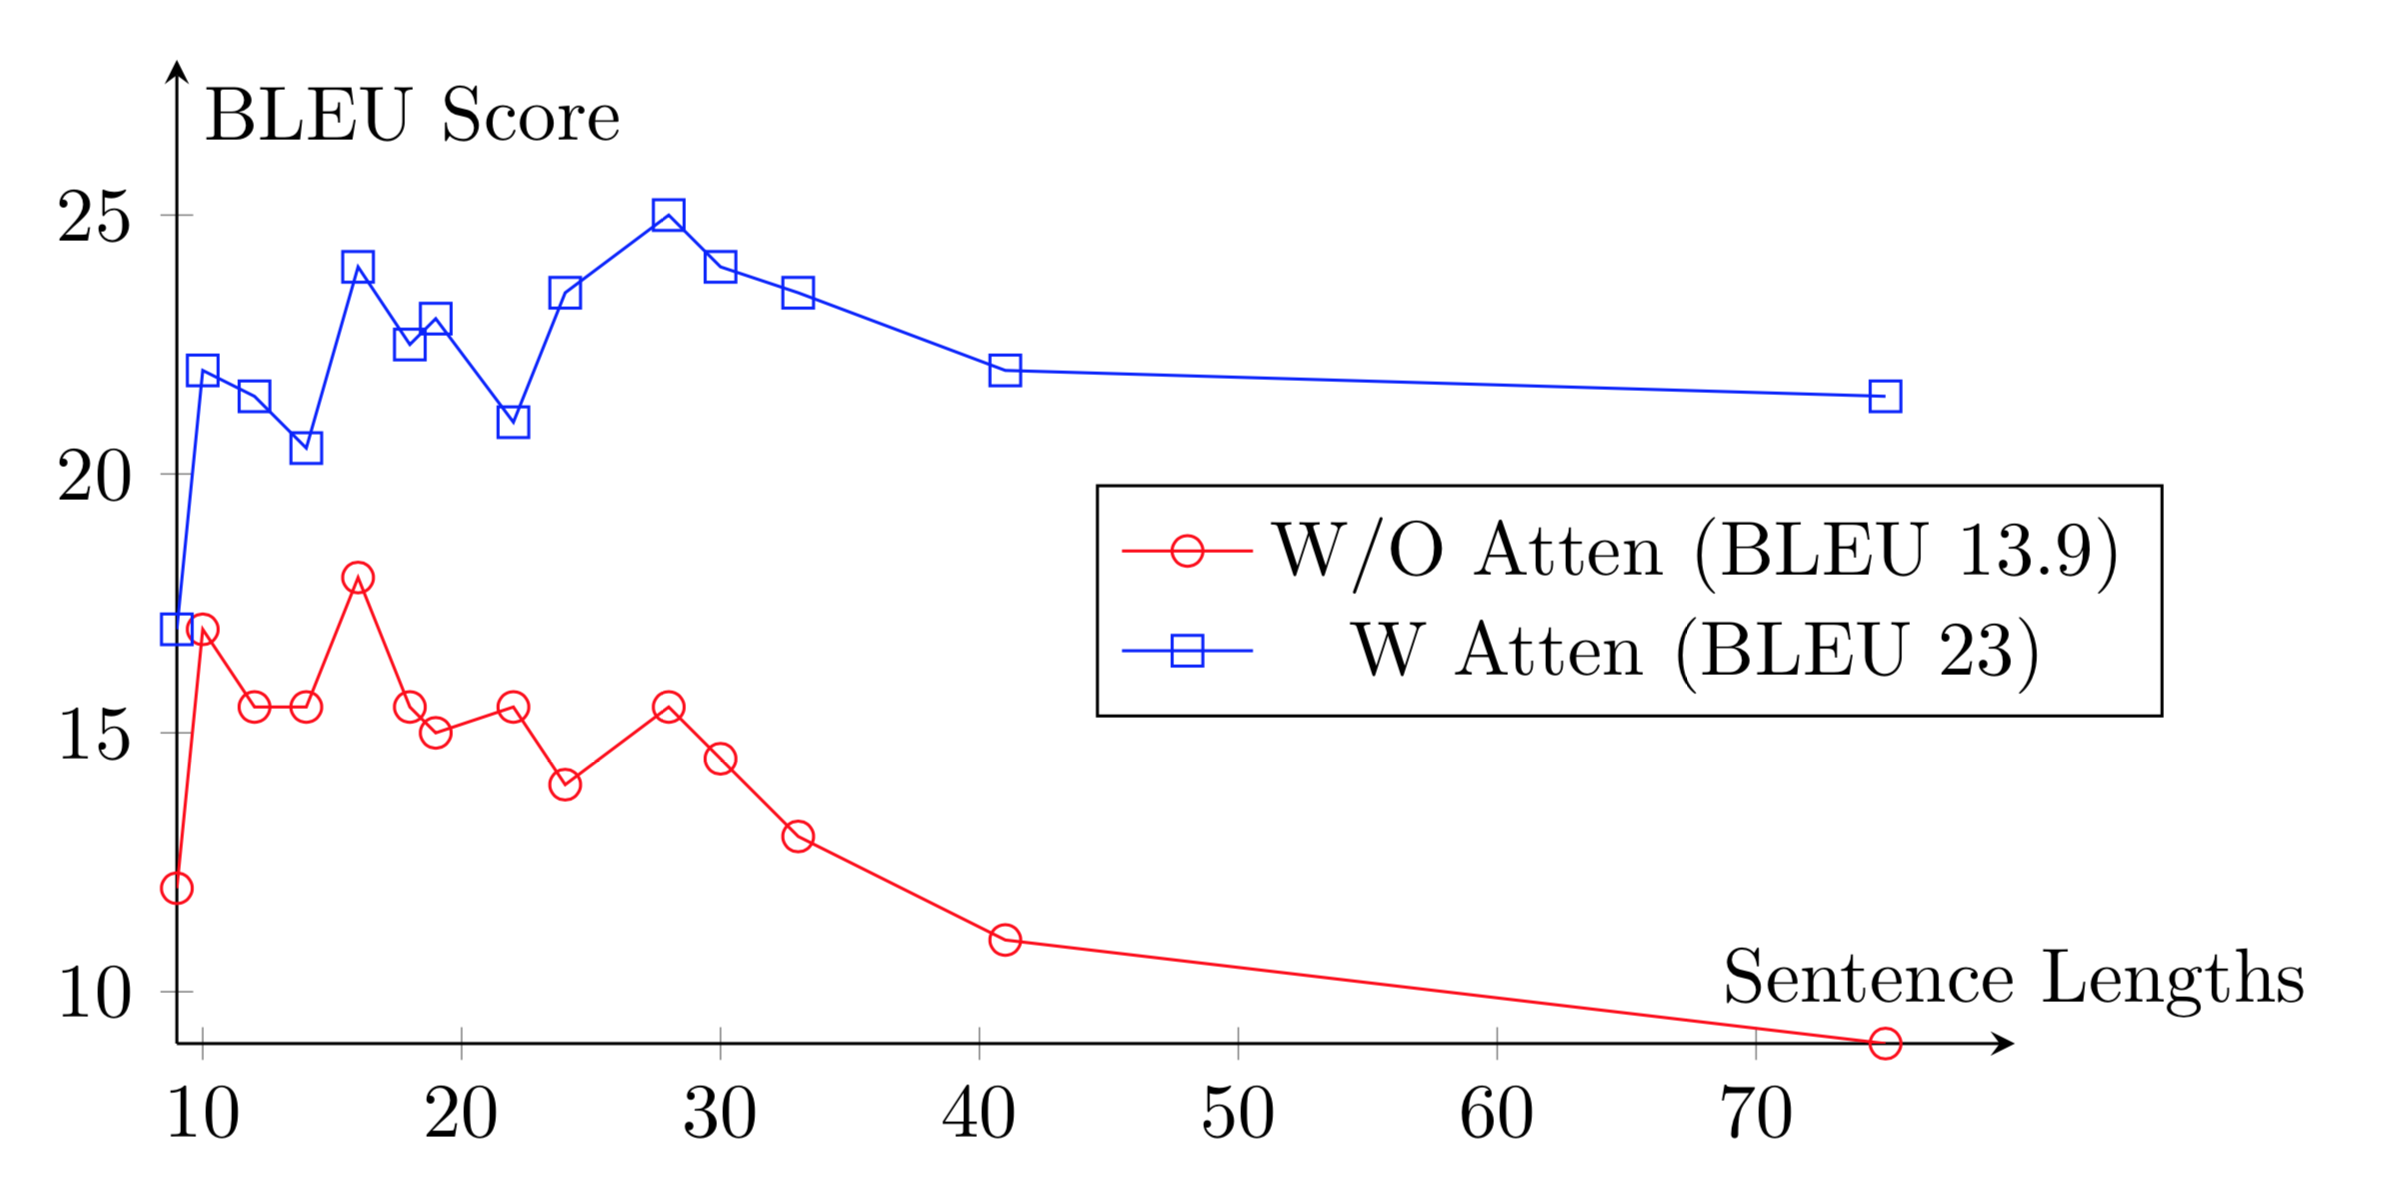
\includegraphics[scale=0.25]{./images/Attention} \\ [-1ex]
    {\tiny Source: Luong et al.\cite{luong:2015:EMNLP}}
    %\caption{Caption}
    \label{fig:att1}
\end{figure}
}

%===================================================================================
\section[SNMT]{Simultaneous NMT}

\frame{
\frametitle{SMT}
\textbf{Simultaneous NMT}
\begin{itemize}
\item Simultaneous Machine Translation is a challenging task of reading from the source language and at the same time, producing the target translation.
\item Many applications:
\begin{itemize}
    \item Broadcast news
    \item Interpretation of lectures, seminars
    \item Political speeches
    \item Customer services
\end{itemize}
\end{itemize}
\hfill 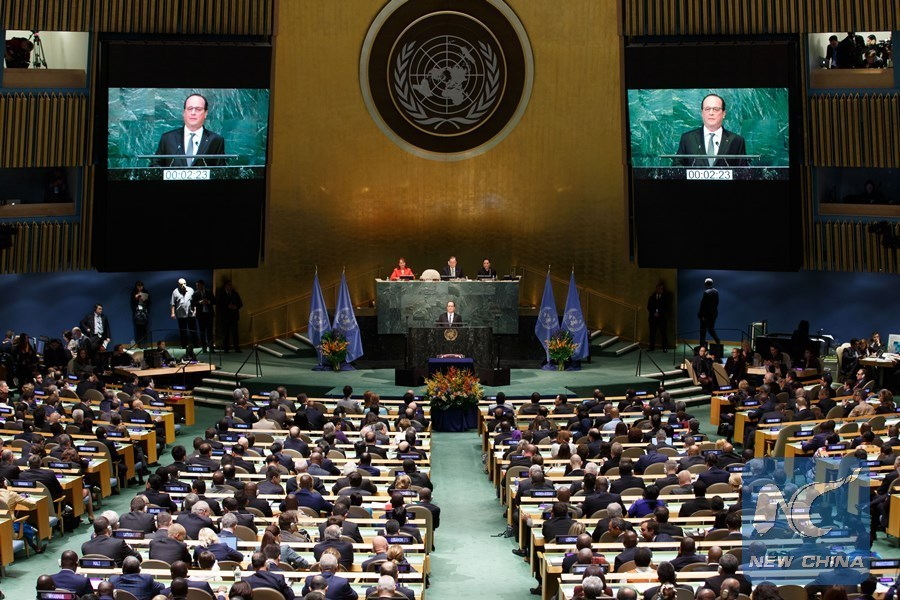
\includegraphics[scale=0.5]{./images/UN}
}

\frame{
\begin{figure}
    \centering
    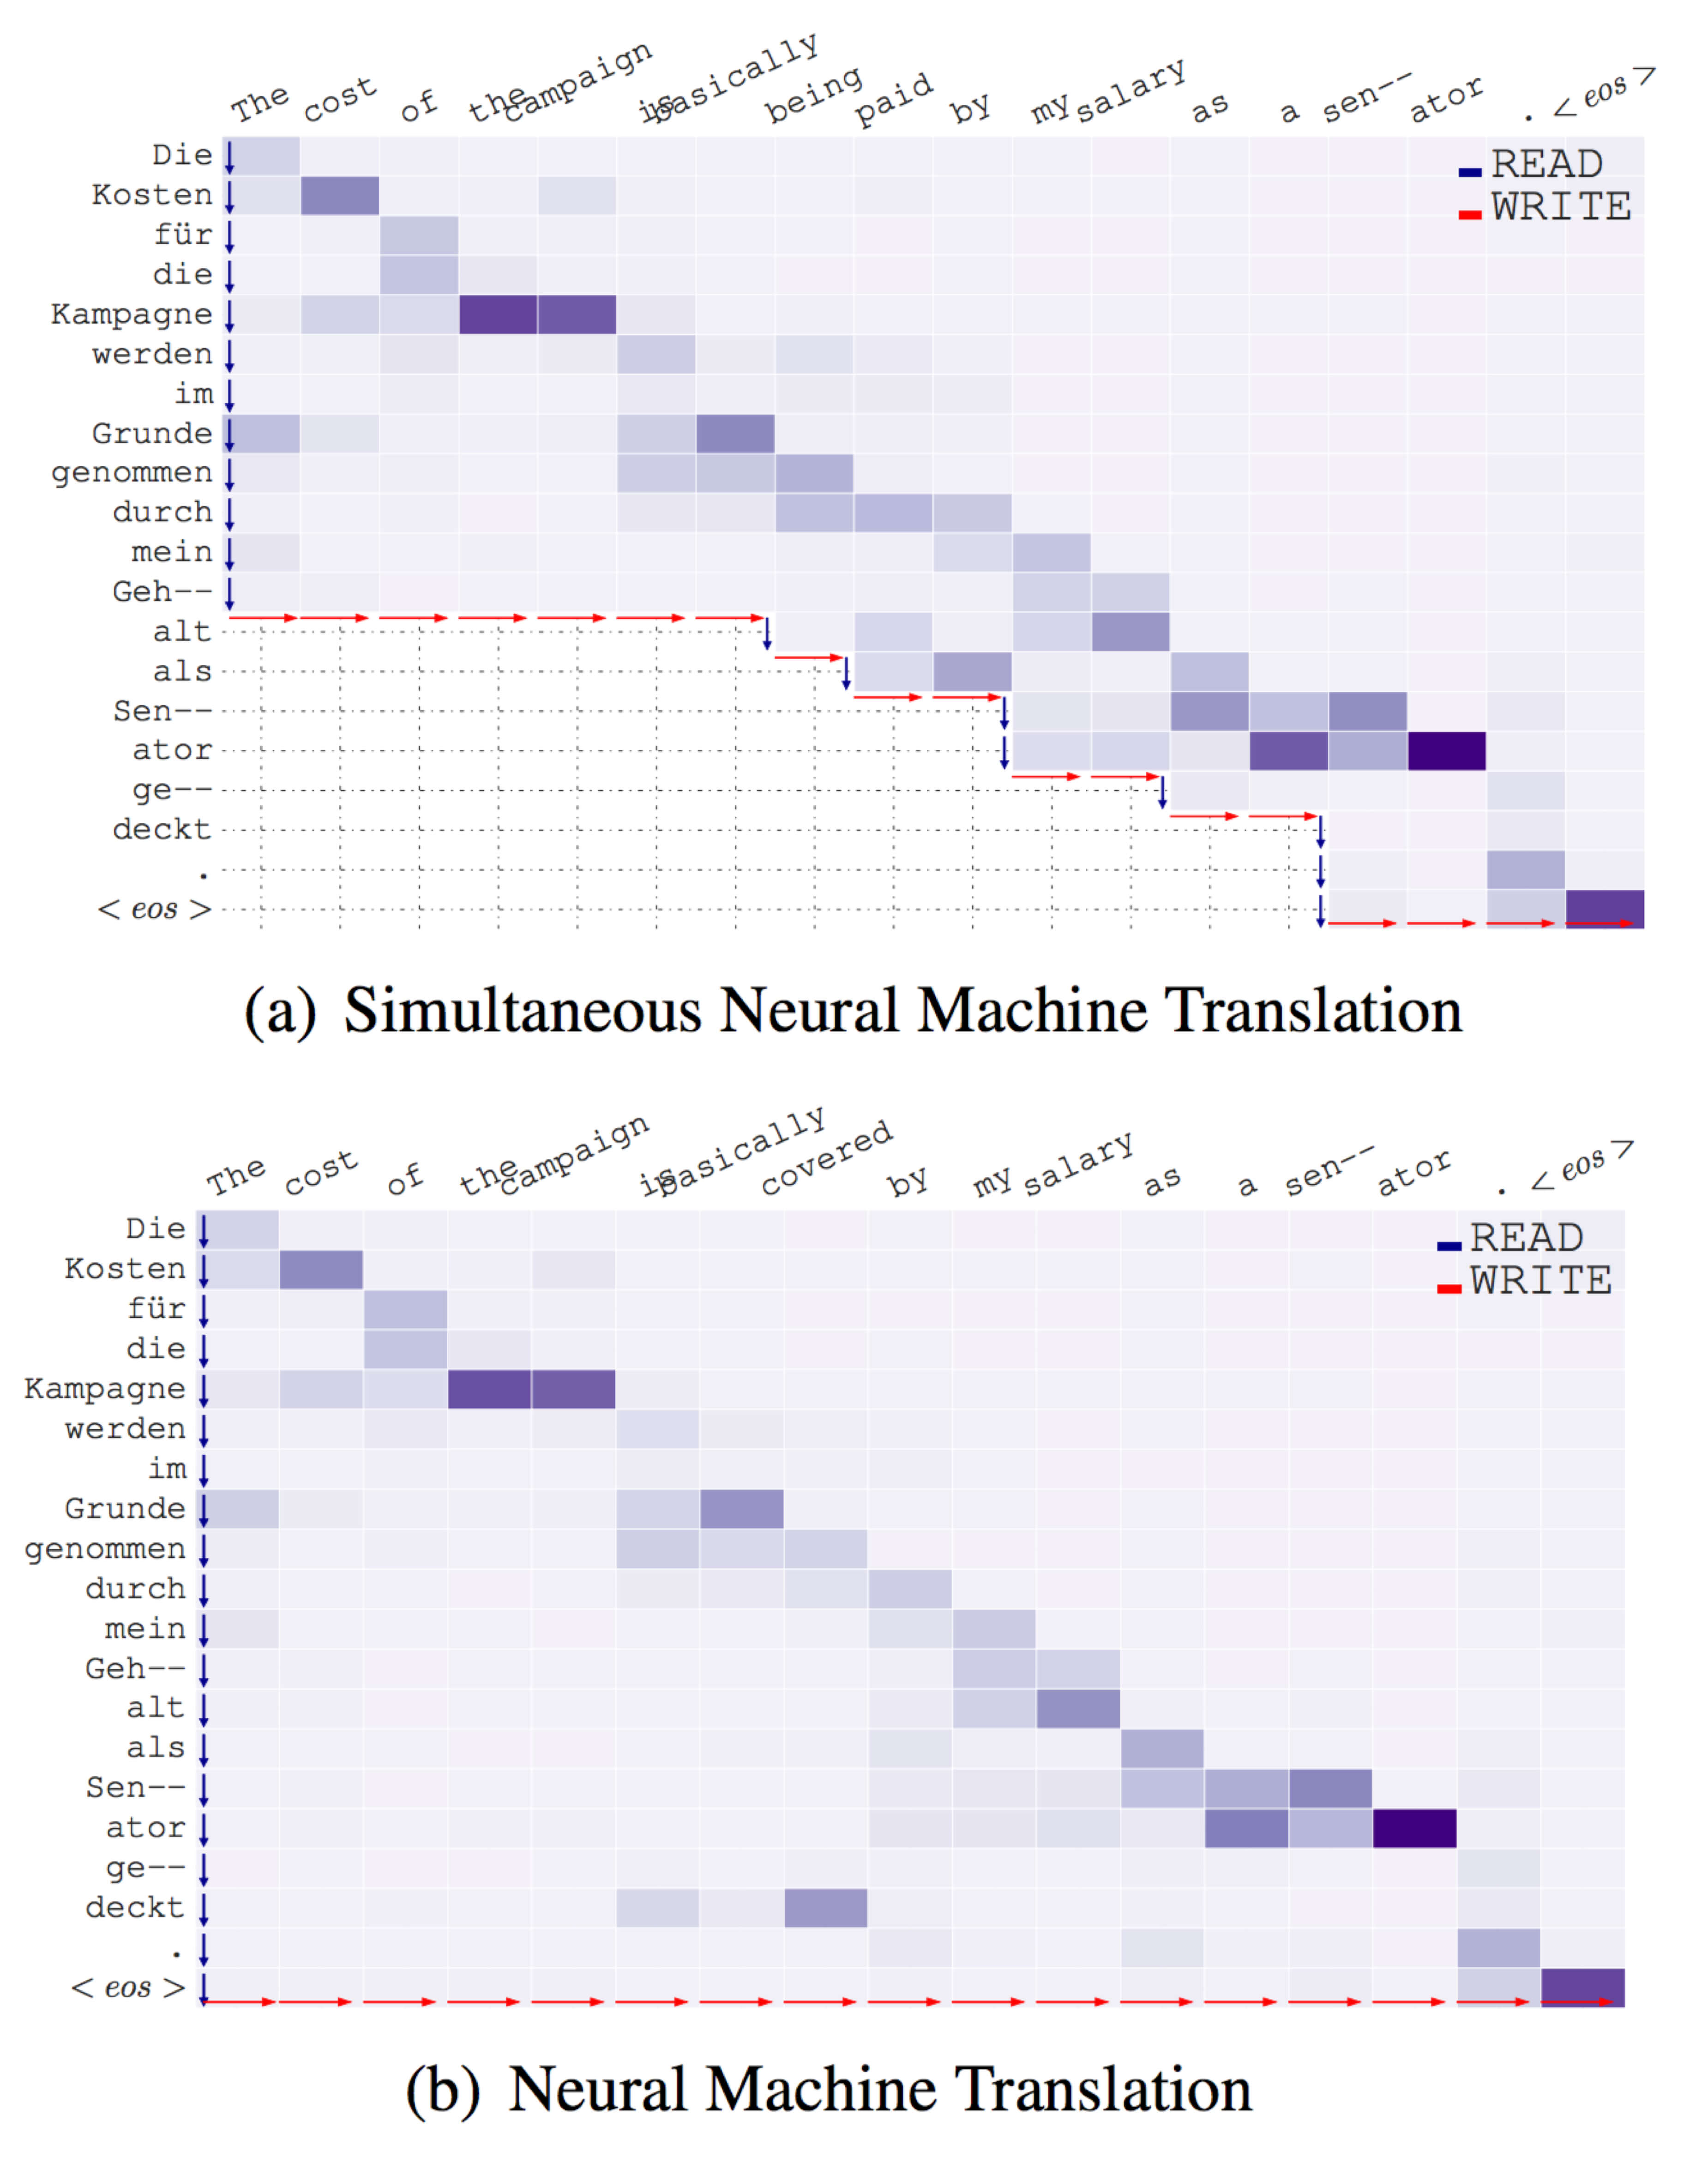
\includegraphics[scale=0.048]{./images/NMTvsSNMT} \\[-1ex]
    {\tiny Source: Gu et al. \cite{gu:2017:EACL}}
    %\caption{Caption}
    \label{fig:smt1}
\end{figure}
}

\frame{
\textbf{Previous works}
\begin{itemize}
\item Most of the works in this direction are done in the context of speech translation. Incoming speech is transcribed and segmented into a translation unit largely based on acoustic and linguistic cues.
\item Each of these segments is then translated largely independent from each other
\end{itemize}
}

\frame{
\textbf{Simultaneous Neural Machine Translation}\\
\vspace{0.2cm}
Two main components:
\begin{enumerate}
    \item Environment
    \item Agent
\end{enumerate}
\begin{figure}
    \centering
    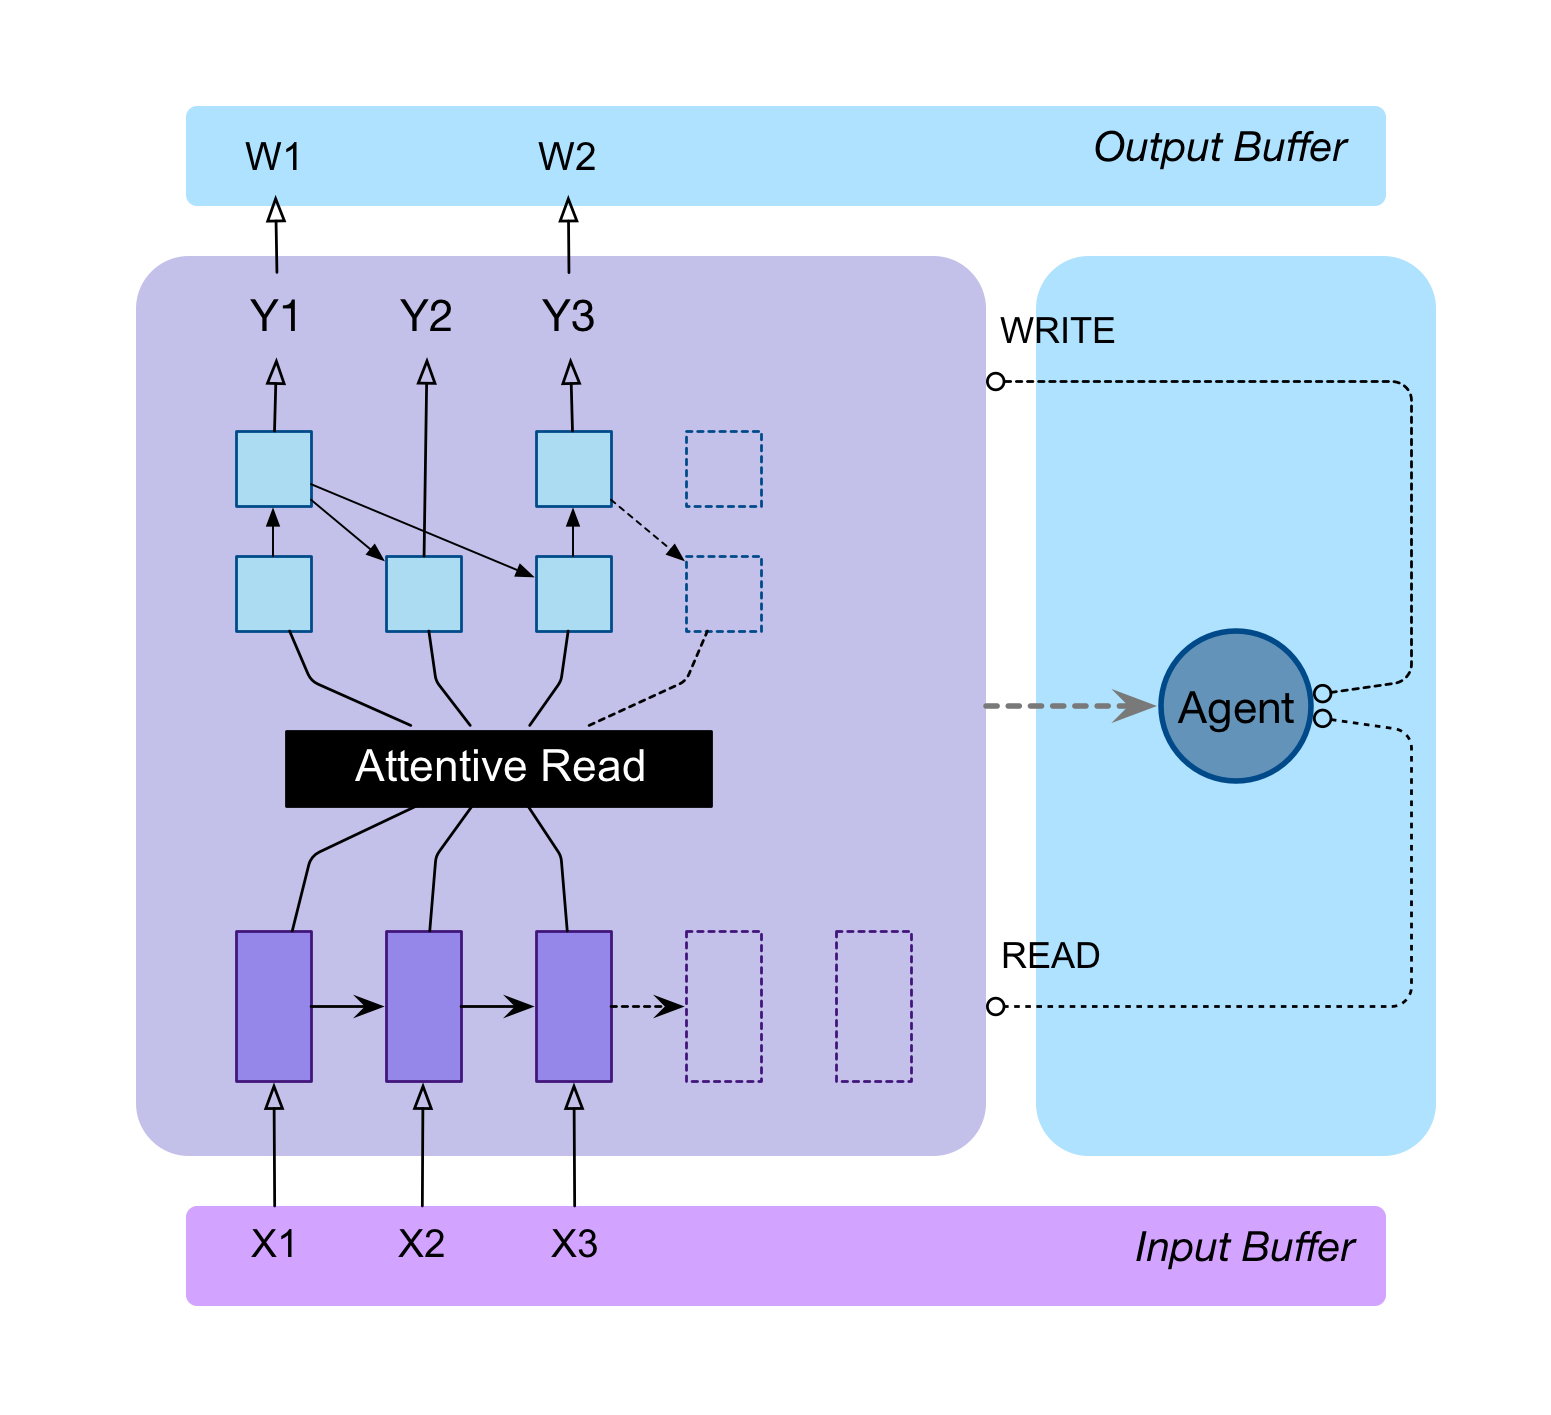
\includegraphics[scale=0.1]{./images/SNMT0} \\[-1ex]
    %\caption{Caption}
    \label{fig:snmt0}
\end{figure}
}

\frame{
\textbf{Simultaneous Neural Machine Translation}
\vspace{5mm}
\begin{itemize}
\item Sequentially making two interleaved decisions:
\begin{enumerate}

\item READ

\item WRITE
\end{enumerate}

\begin{center}
\begin{equation*}
\begin{aligned}
\text{Input sequence} & \ \ \  X = \{ x_1, \dots, x_{T_x} \} \\
\text{Decoded Output} & \ \ \ W = \{ w_1, \dots, w_{T_w} \} \\
\text{Action sequence} & \ \ \  A = \{ a_1, \dots, a_{T} \} \\
\vspace{10cm} \\
T &= T_x + T_w
\phantom{\hspace{0cm}}
\end{aligned}
\end{equation*}
\end{center}

\end{itemize}
}

\frame{
\only<1>{
\textbf{Metrics}
\begin{itemize}
\item \textbf{Quality} The metrics for evaluating quality of the translation is the BLEU score.
\end{itemize}
$$\text{BLEU} = \left( \prod_{n=1}^{4} \frac{\# \ \text{of matched n-grams}}{\text{Total}\ \#\ \text{of n-grams}} \right)^{\frac{1}{4}} \times 100$$

\vspace{0.5cm}
}

\only<2>{
\textbf{Metrics}
\begin{itemize}
\item \textbf{Quality} The metrics for evaluating quality of the translation is the BLEU score.
\end{itemize}
$$\text{BLEU} = \left( \prod_{n=1}^{4} \frac{\# \ \text{of matched n-grams}}{\text{Total}\ \#\ \text{of n-grams}} \right)^{\frac{1}{4}} \times 100$$

\vspace{0.5cm}
EX : 
\begin{center}
 (ref) \textcolor{darkblue}{ This is small test }\\

(cand1) This is a test \\

$$ \text{1-gram}: 0.75 \quad \text{2-gram}: 0.33 \quad \text{3-gram and 4-gram}: 0$$
\end{center}
}

\only<3>{
\textbf{Metrics}
\begin{itemize}
\item \textbf{Quality} The metrics for evaluating quality of the translation is the BLEU score.
\end{itemize}
$$\text{\textcolor{red}{Smooth-}BLEU} = \left( \prod_{n=1}^{4} \frac{\# \ \text{of matched n-grams \textcolor{red}{+1} }}{\text{Total}\ \#\ \text{of n-grams \textcolor{red}{+1} }} \right)^{\frac{1}{4}} \times 100$$

\vspace{0.5cm}
EX : 
\begin{center}
 (ref) \textcolor{darkblue}{ This is small test }\\

(cand1) This is a test \\

$$ \text{1-gram}: 0.75 \quad \text{2-gram}: 0.33 \quad \text{3-gram and 4-gram}: \textcolor{red}{1}$$
\end{center}
}

\only<4>{
\textbf{Metrics}
\begin{itemize}
\item \textbf{Quality} The metrics for evaluating quality of the translation is the BLEU score.
\end{itemize}
$$\text{Smooth-BLEU} = \left( \prod_{n=1}^{4} \frac{\# \ \text{of matched n-grams +1 }}{\text{Total}\ \#\ \text{of n-grams +1 }} \right)^{\frac{1}{4}} \times 100$$

\vspace{0.5cm}
EX : 
\begin{center}
 (ref) \textcolor{darkblue}{ This is small test }\\
\end{center}
\begin{align*}
\text{(cand1) This is a test} \qquad &\text{BLEU} = 24.75\\
\text{(cand2) This is small test} \qquad &\text{BLEU} = 100\\
\text{(cand3) The big exam} \qquad &\text{BLEU} = 0\\
\end{align*}
}
}

\frame{
\textbf{Delay}
\begin{itemize}
    \item \textbf{Average Proportion (AP)}
    $s(t) = $ In each time step for the decoded target symbol $\hat{y}_t$, how many source symbols were required.
    \vspace{-0.5cm}
    \begin{center}
    \begin{align*}
        &\text{R \quad R \quad R \quad W \quad W \quad R \quad W \quad W}\\
        &\ \ \ \quad \ \ \ \quad \ \ \ \quad 3\ \ \quad\ 3\ \ \quad \ \ \ \quad 4\ \ \quad 4 \ \ =\ \ \frac{14}{16}
    \end{align*}
    \end{center}
    
%$$ 0 < T(X, \hat{Y}) = \frac{1}{|X||\hat{Y}|} \sum^{|\hat{y}|}_{t=1} s(t) \leq 1. $$

    \item \textbf{Consecutive Wait (CW)}
    
    \vspace{-0.5cm}
    \begin{center}
    \begin{align*}
        &\text{R \quad R \quad R \quad W \quad W \quad R \quad W \quad W}\\
        &1\ \ \quad 2\ \quad 3\ \ \quad 0\ \ \quad 0\ \ \quad 1\ \ \quad 0\ \ \quad 0
    \end{align*}
    \end{center}
    % \begin{align*}
    %    c_t = 
    %    \begin{cases}
    %    c_{t-1} + 1 & a_t = \text{READ}\\
    %    0           & a_t = \text{WRITE}
    %    \end{cases}
    %\end{align*}
    \item \textbf{Wait Delay}
    $$ r_t^D = 1 - \frac{\text{CW}-1}{\lambda}$$
\end{itemize}
}

\subsection[Environment]{$\diamond$ Environment}


%\frame{
%\begin{center}
%\Huge Simultaneous NMT
%\end{center}
%}

%\frame{
%http://www.systransoft.com/systran/translation-technology/what-is-machine-translation/
%\begin{itemize}
%\item Machine Translation is the process by which computer software is used to translate a text from %one natural language (such as English) to another (such as Spanish).
%\item Three main methods:
%\begin{enumerate}
%\item Rule-Based Machine Translation.
%\item Statistical Machine Translation.
%\item Neural Machine Translation.
%\end{enumerate}
%\end{itemize}
%

\frame{
\only<1>{
\textbf{Environment}\\
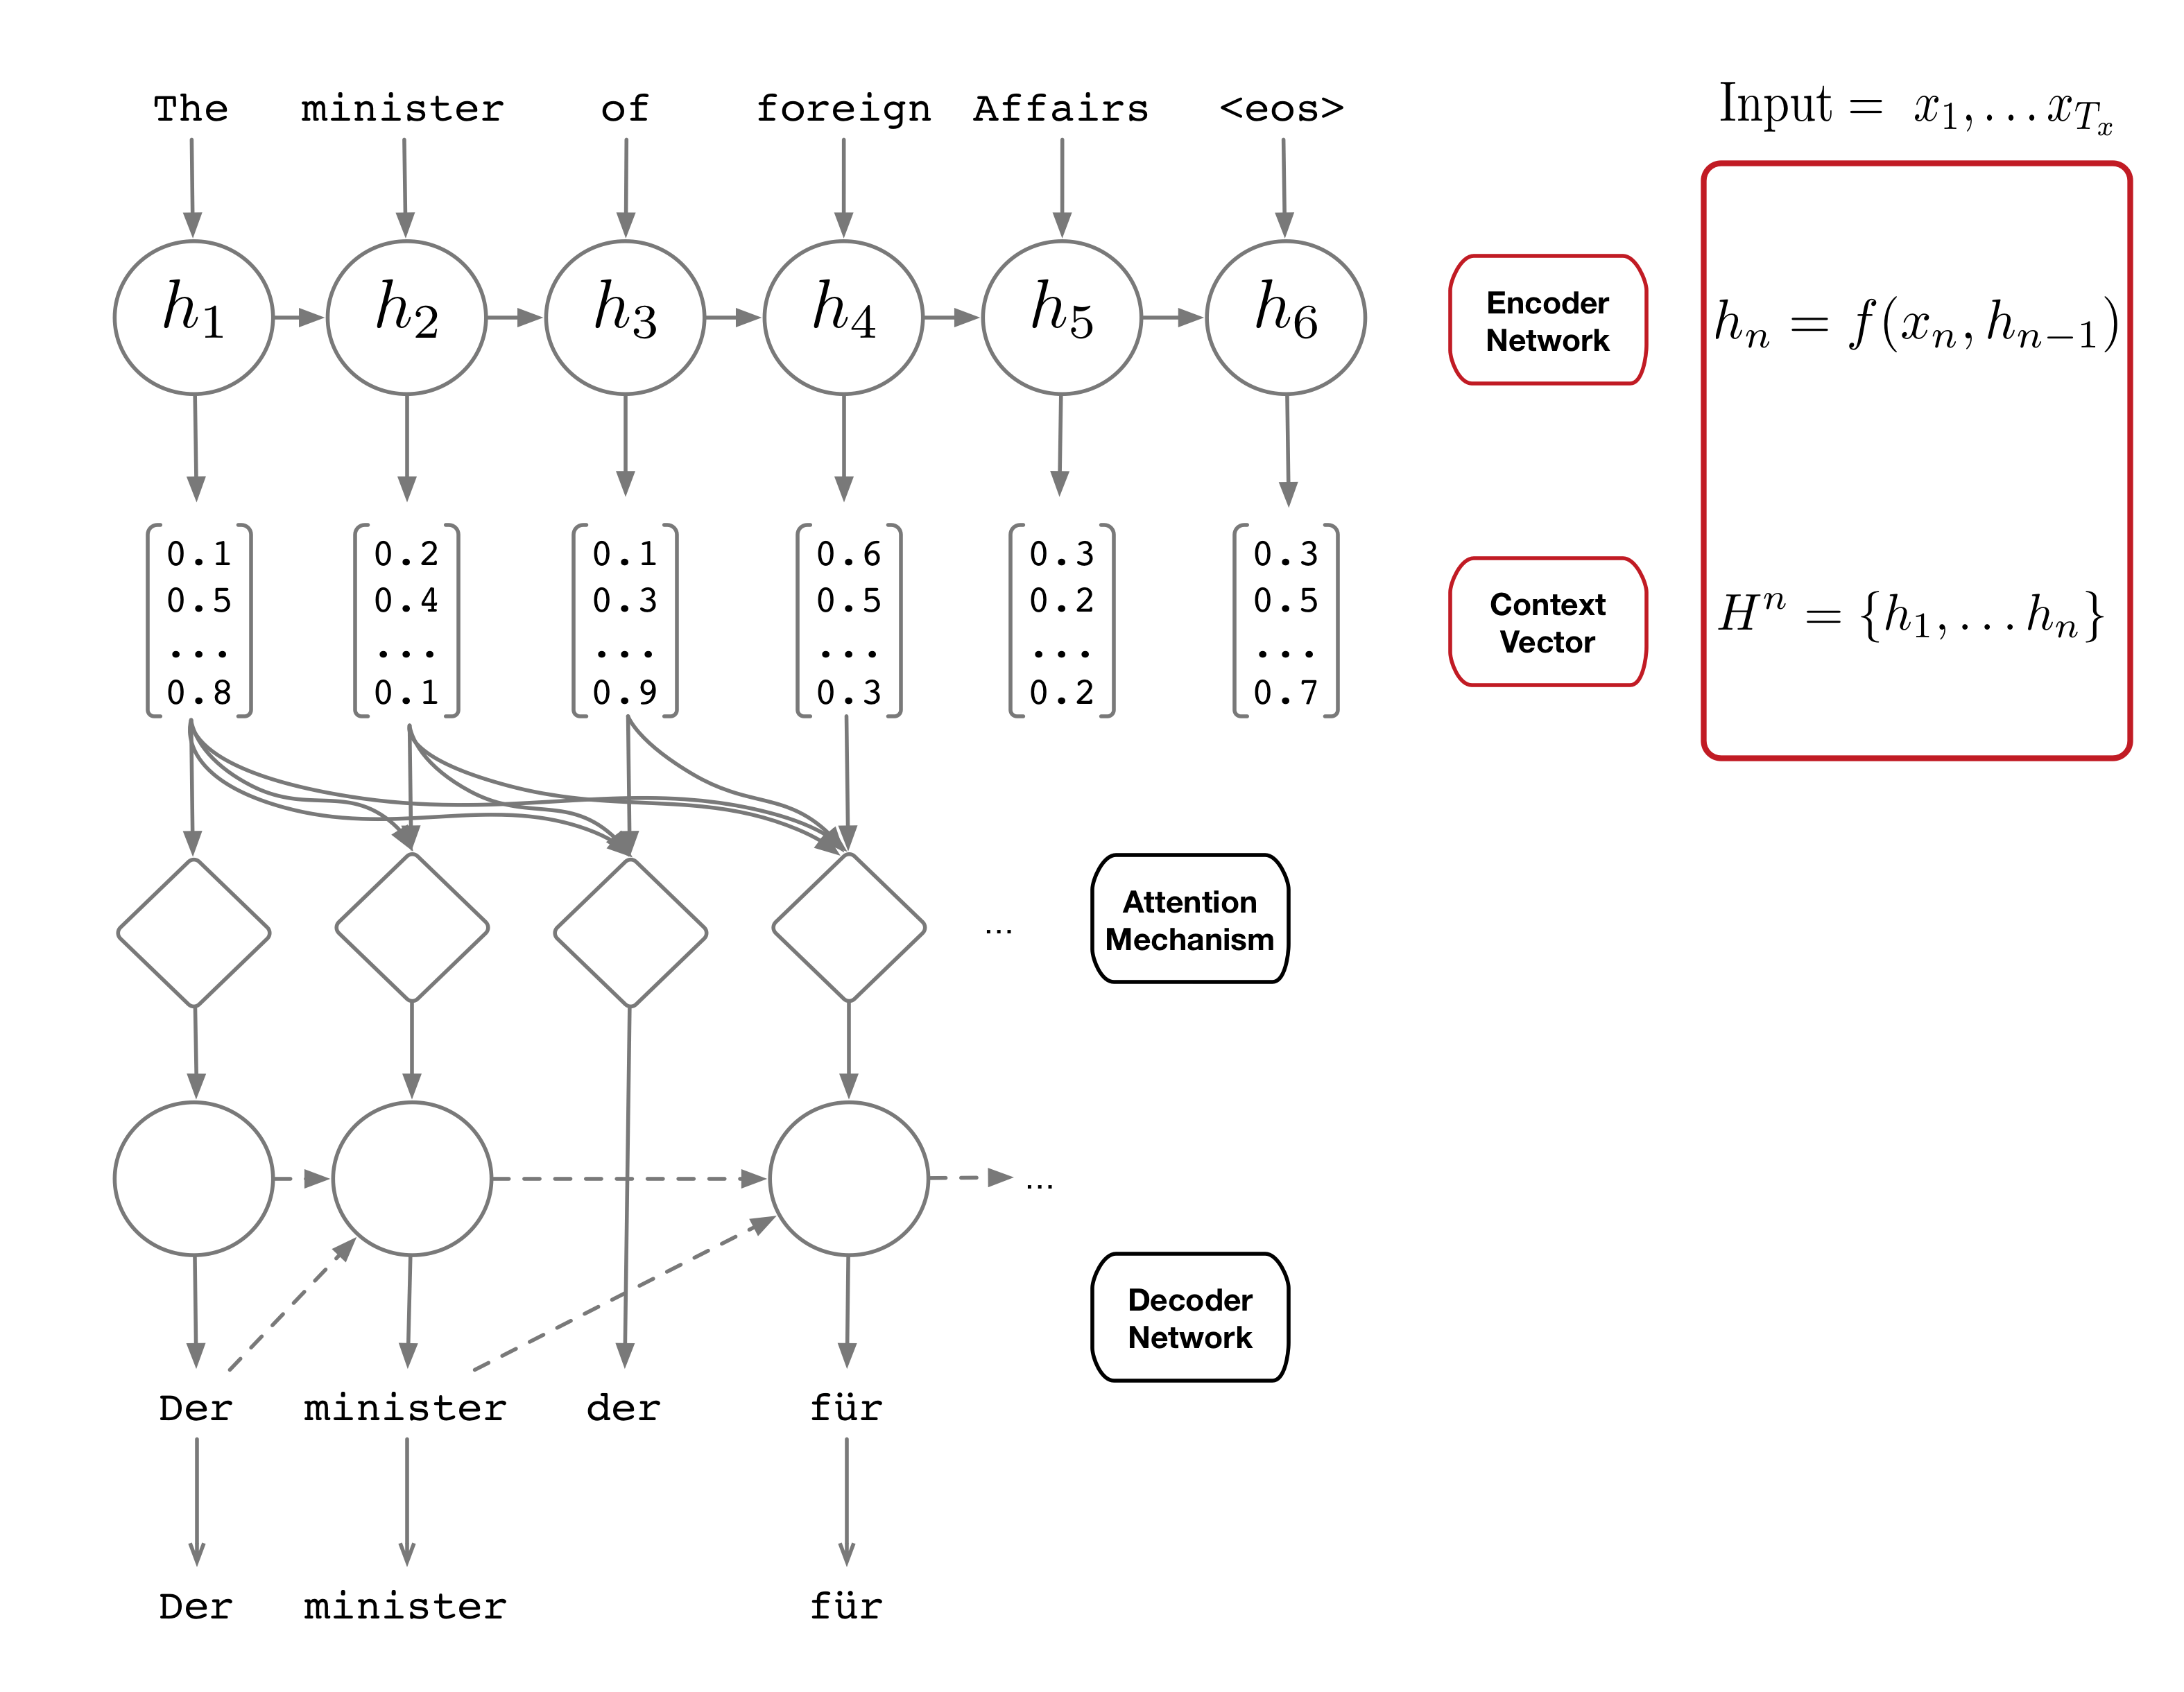
\includegraphics[scale=0.09]{./images/env1}
}
\only<2>{
\textbf{Environment}\\
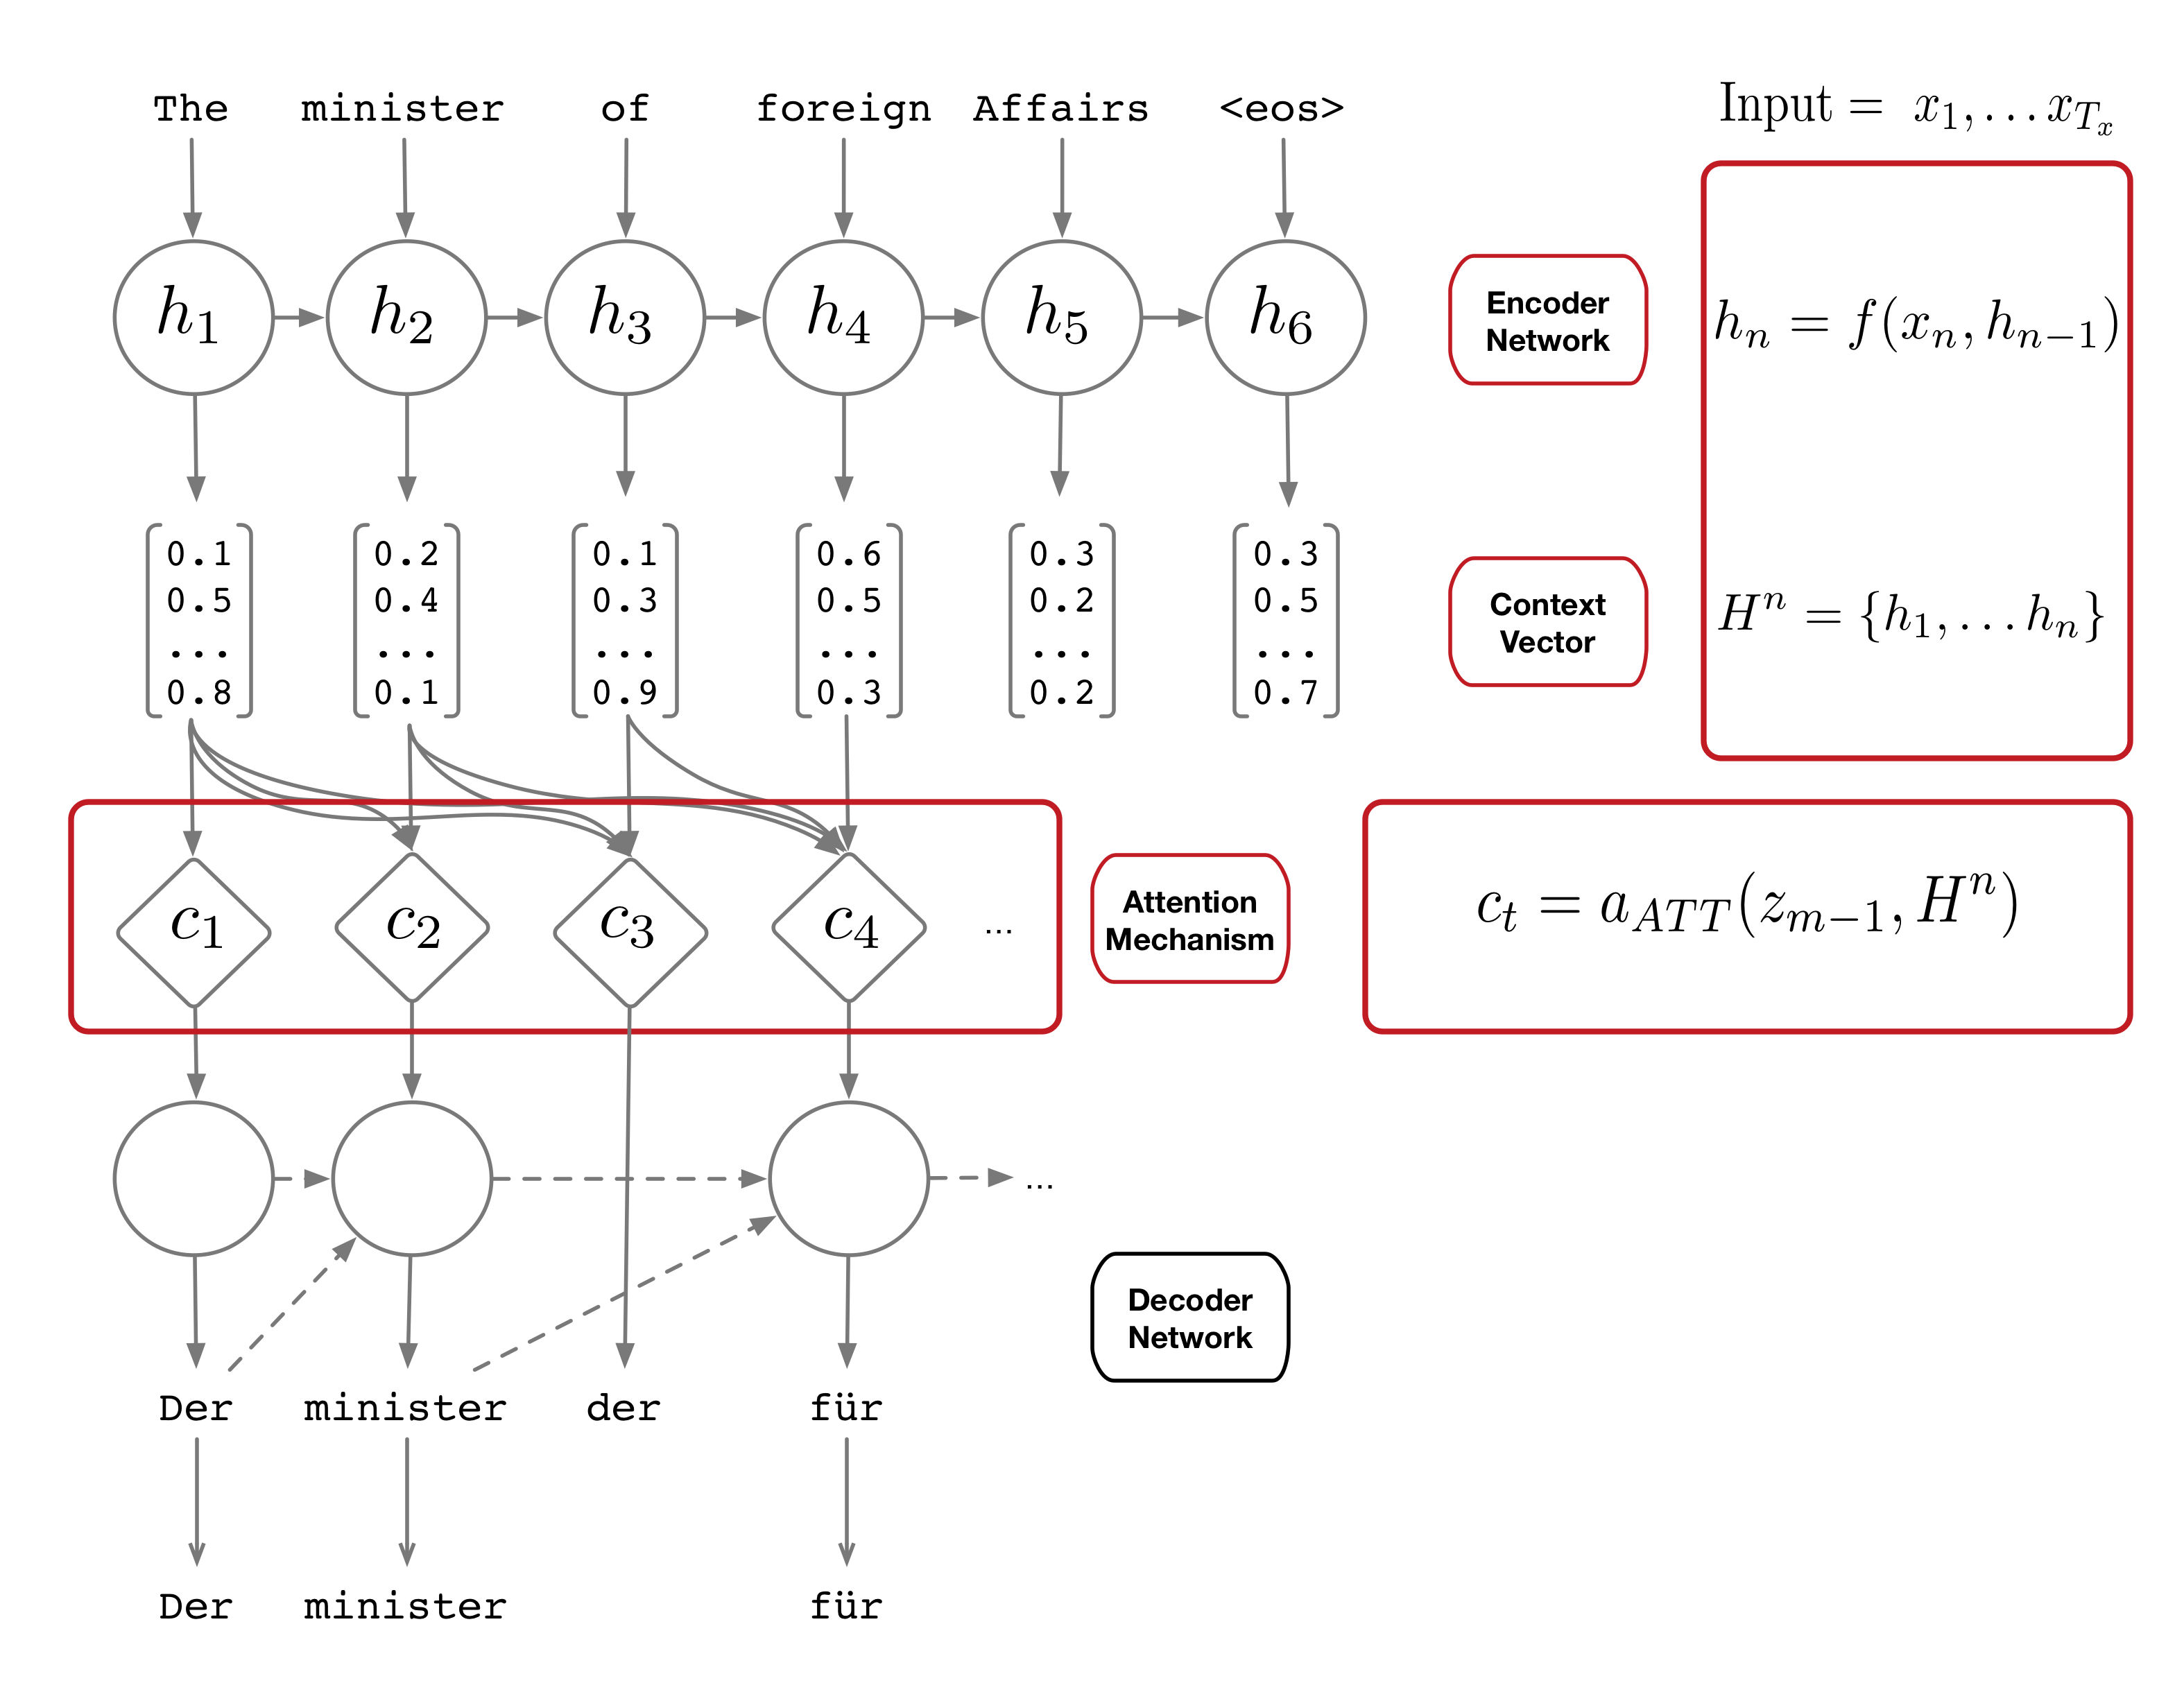
\includegraphics[scale=0.09]{./images/env2}
}
\only<3>{
\textbf{Environment}\\
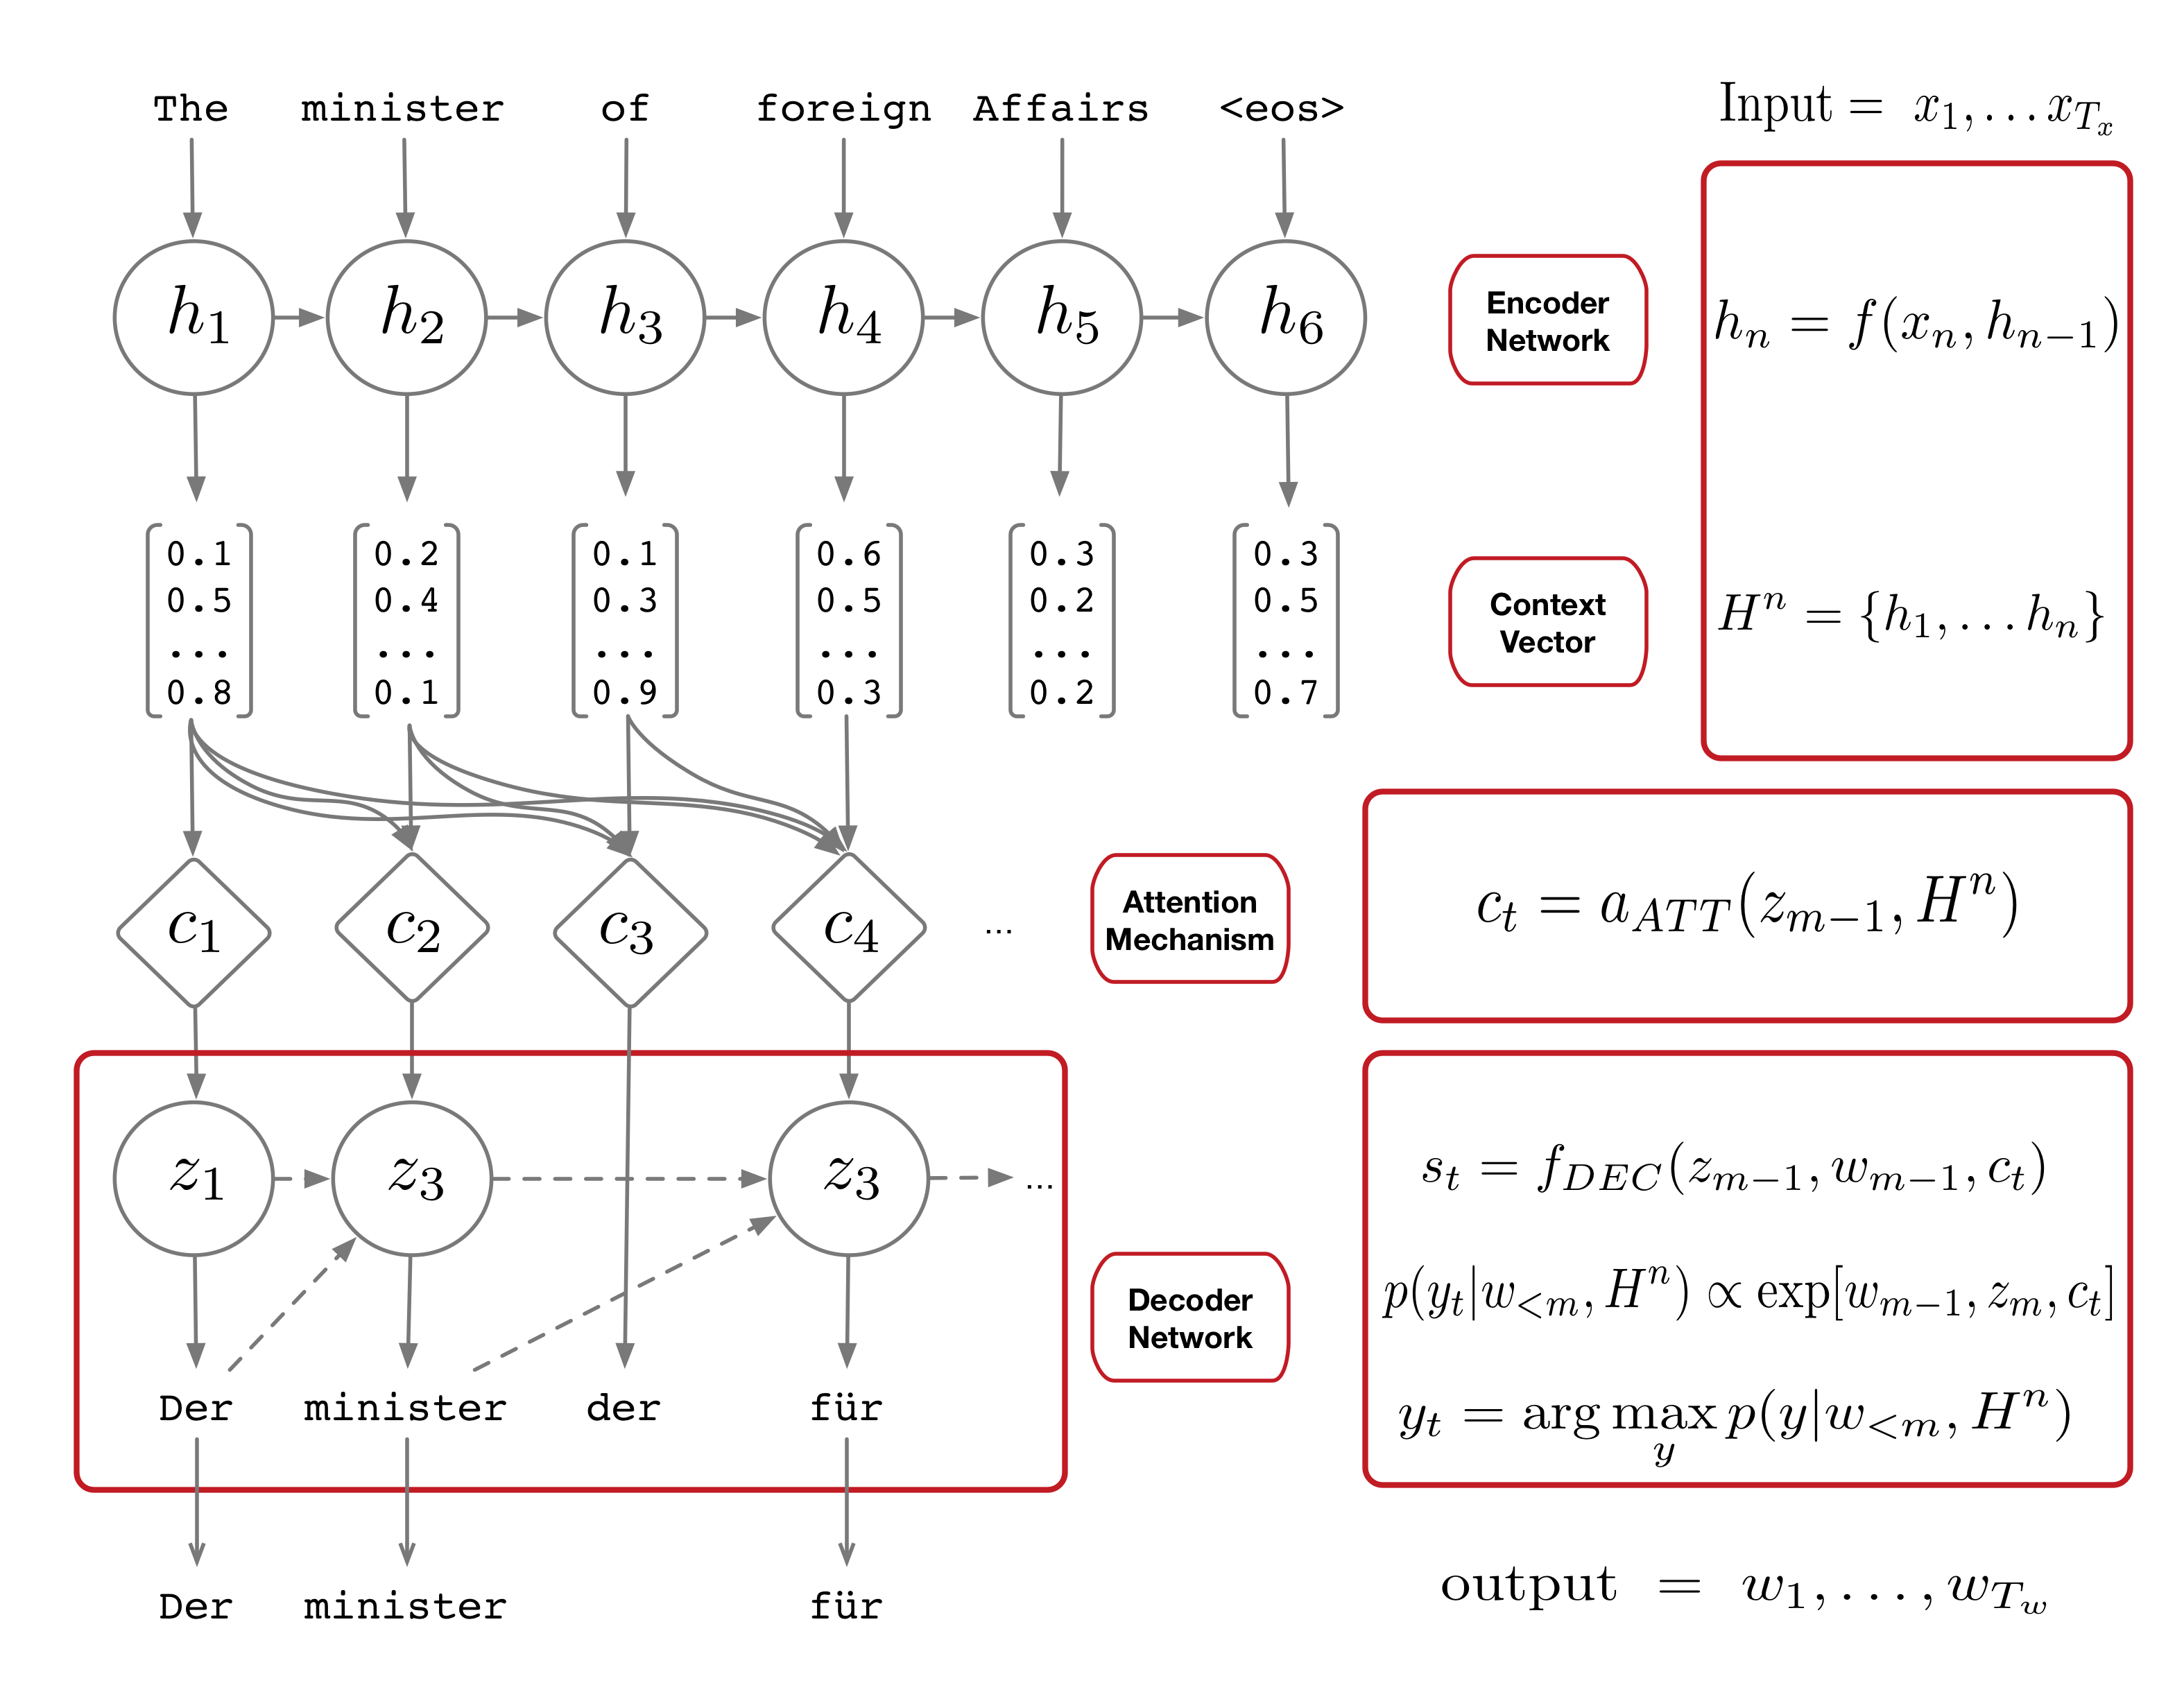
\includegraphics[scale=0.09]{./images/env3}
}
}

\subsection[Agent]{$\diamond$ Agent}

\frame{
\textbf{The Agent}
\begin{itemize}
    \item Greedy Decoding
    \item Q-network
    \item Policy Gradient
\end{itemize}
}

%\frame{
%\centering
%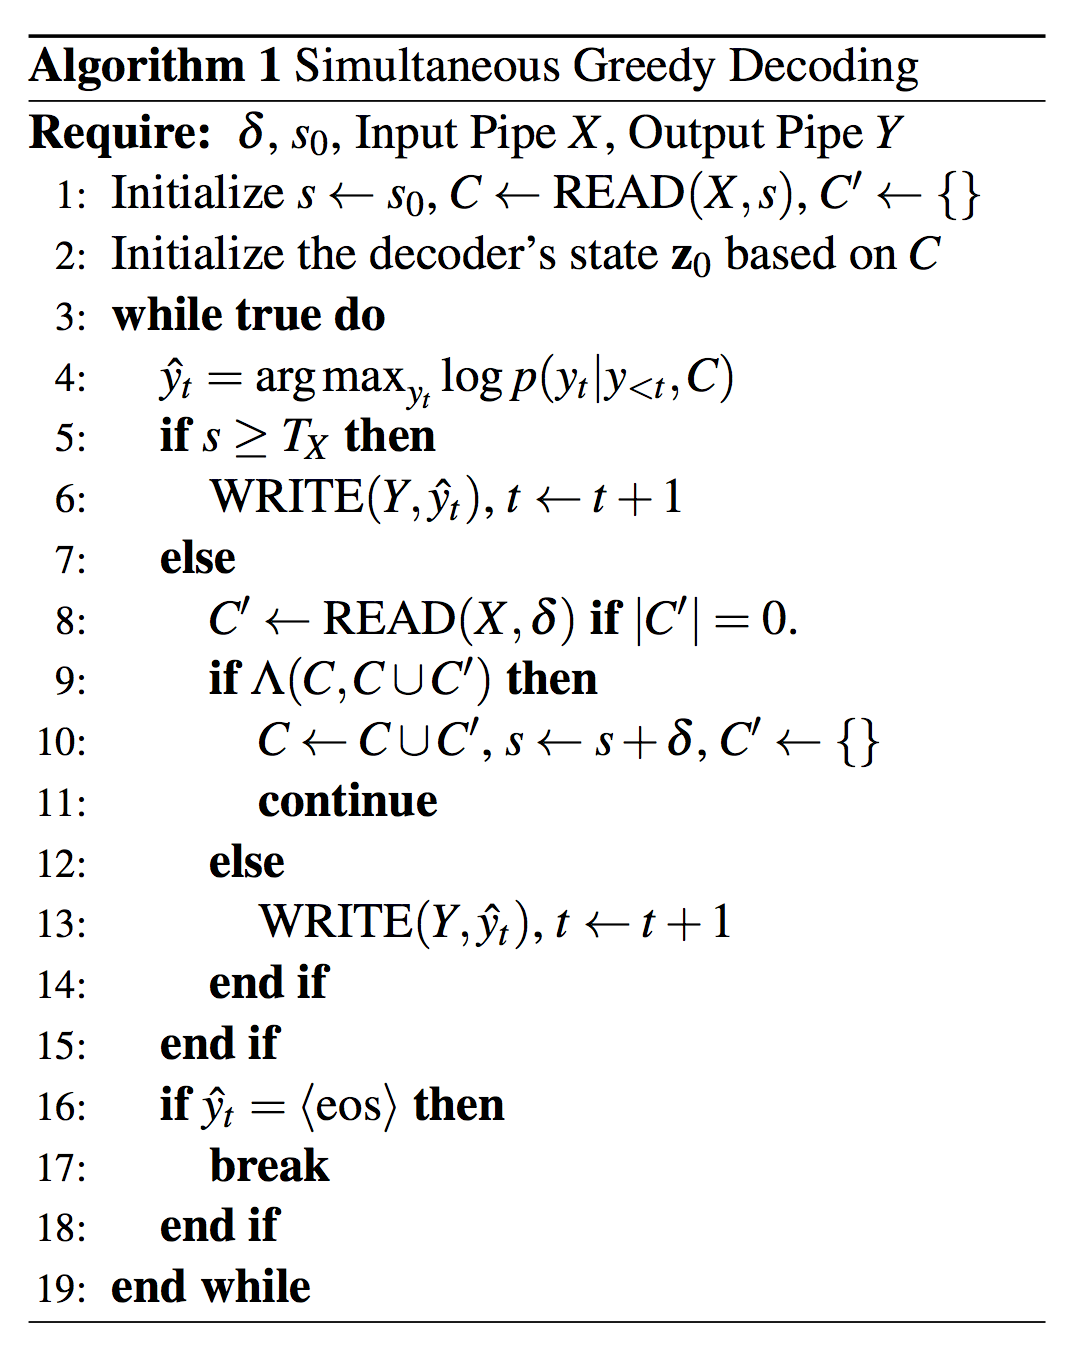
\includegraphics[scale=0.32]{./images/GD}
%}


\subsubsection[Greedy Decoding]{- Greedy Decoding}

\frame{
\textbf{Greedy Decoding} \hfill [Cho et al., 2016]\\

\begin{itemize}
\item \textbf{Wait-If-Worse} \\

\vspace{1cm}
\scalebox{0.8}{
\begin{equation*}
\begin{aligned}
    \Lambda(t) = 
    \begin{cases}
    \text{ READ} & \text{if} \ \log p(y_t|w_{<{m}}, H^n) < \log p(y_t|w_{<{m}}, H^{n+1})\\
    \text{ WRITE} & \text{otherwise}
    \end{cases}
    \vspace{10cm}                           
\end{aligned}
\end{equation*}
}
\vspace{1cm}
\item \textbf{Wait-If-Diff}\\

\vspace{1cm}
\scalebox{0.8}{
\begin{equation*}
\begin{aligned}
    \Lambda(t) = 
    \begin{cases}
    \text{READ} & \text{if} \ y_t \neq y_{t+1}\\
    \text{WRITE} & \text{otherwise}
    \end{cases}
    \vspace{10cm} 
\end{aligned}
\end{equation*}
}

\end{itemize}
}
%%%%%%%%%%%
\frame{

\only<1>{
\centering{
\textbf{\textcolor<1>{darkblue}{The minister of }}\textcolor<1>{lightblue}{foreign affairs says Germany is ...} \\
\vspace{1cm}
\footnotesize Der minister \textcolor<1>{grey}{von}\\
}
\begin{center}
\begin{align*}
    &{\scriptstyle \log p(\text{von} | y_{<t}, \text{The minister of}) = 0.432}\\[-0.5ex]
\end{align*}
\end{center}
}

\only<2>{
\centering{
\textbf{\textcolor<2>{darkblue}{The minister of foreign }}\textcolor<2>{lightblue}{affairs says Germany is ...} \\
\vspace{1cm}
\footnotesize Der minister \textcolor<2>{grey}{der fremden}\\
}
\begin{center}
\begin{align*}
    &{\scriptstyle \log p(\text{von} | y_{<t}, \text{The minister of}) = 0.432} \\[-0.5ex]
    &{\scriptstyle \log p(\text{der} | y_{<t}, \text{The minister of foreign}) = 0.425}
\end{align*}
\end{center}
}

\only<3>{
\centering{
\textbf{\textcolor<3>{darkblue}{The minister of foreign affairs }}\textcolor<3>{lightblue}{says Germany is ...} \\
\vspace{1cm}
\footnotesize Der minister \textcolor<3>{grey}{f\"{u}r ausw\"{a}rtige}\\
}
\begin{center}
\begin{align*}
    &{\scriptstyle \log p(\text{der} | y_{<t}, \text{The minister of foreign}) = 0.425}\\[-0.5ex]
    &{\scriptstyle \log p(\text{f\"{u}r} | y_{<t}, \text{The minister of foreign affairs}) = 0.57}
\end{align*}
\end{center}
}

\only<4>{
\centering{
\textbf{\textcolor<4>{darkblue}{The minister of foreign affairs says }}\textcolor<4>{lightblue}{Germany is ...} \\
\vspace{1cm}
\footnotesize Der minister f\"{u}r \textcolor<4>{grey}{ausw\"{a}rtige}\\
}
\begin{center}
\begin{align*}
    &{\scriptstyle \log p(\text{f\"{u}r} | y_{<t}, \text{The minister of foreign affairs}) = 0.57}\\[-0.5ex]
    &{\scriptstyle \log p(\text{f\"{u}r} | y_{<t}, \text{The minister of foreign affairs says}) = 0.57}
\end{align*}
\end{center}
}
}
%%%%%%%%%%%%%

\frame{
\begin{figure}
    \centering
    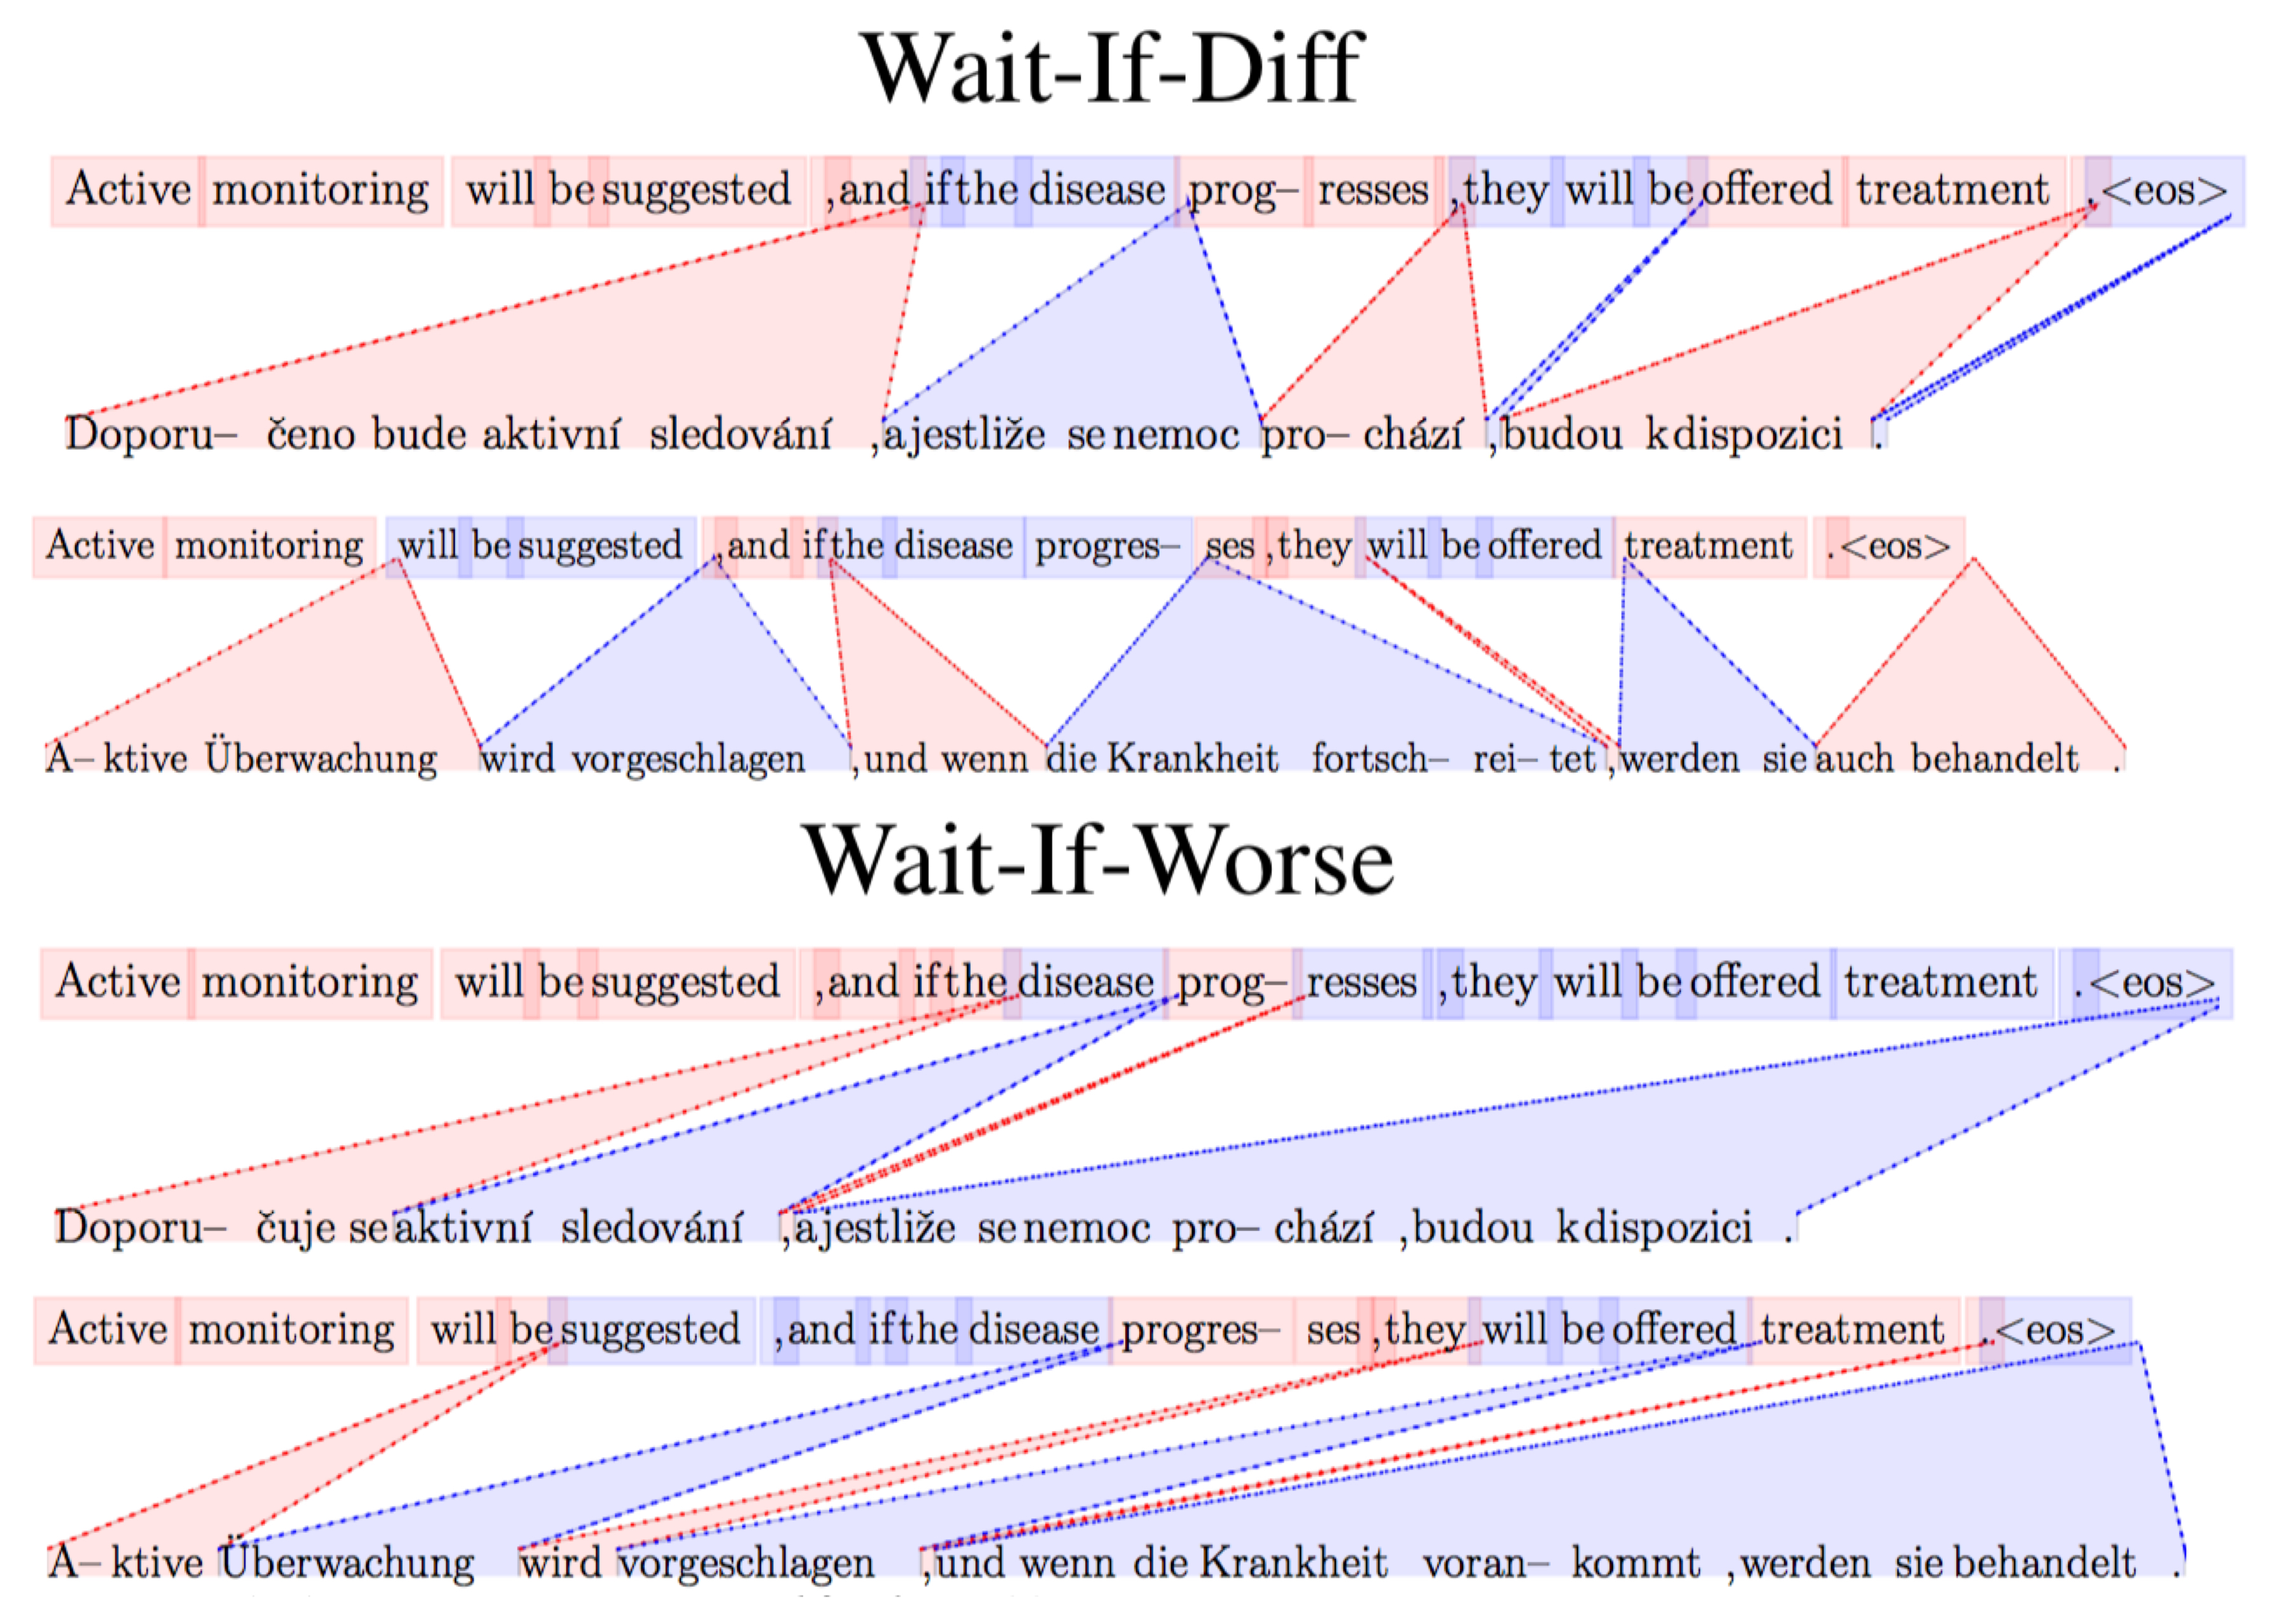
\includegraphics[scale=0.07]{./images/WIWWID2} \\[-1ex]
    {\raggedleft \tiny Source: Cho et al.\cite{cho:2016:Arxive}}
    \caption{From English:"\textit{Active monitoring will be suggested, and if the disease progresses, they will be offered treatment.}"}
    \label{fig:WID}
\end{figure}
}

%\frame{
%\begin{figure}
%\centering
%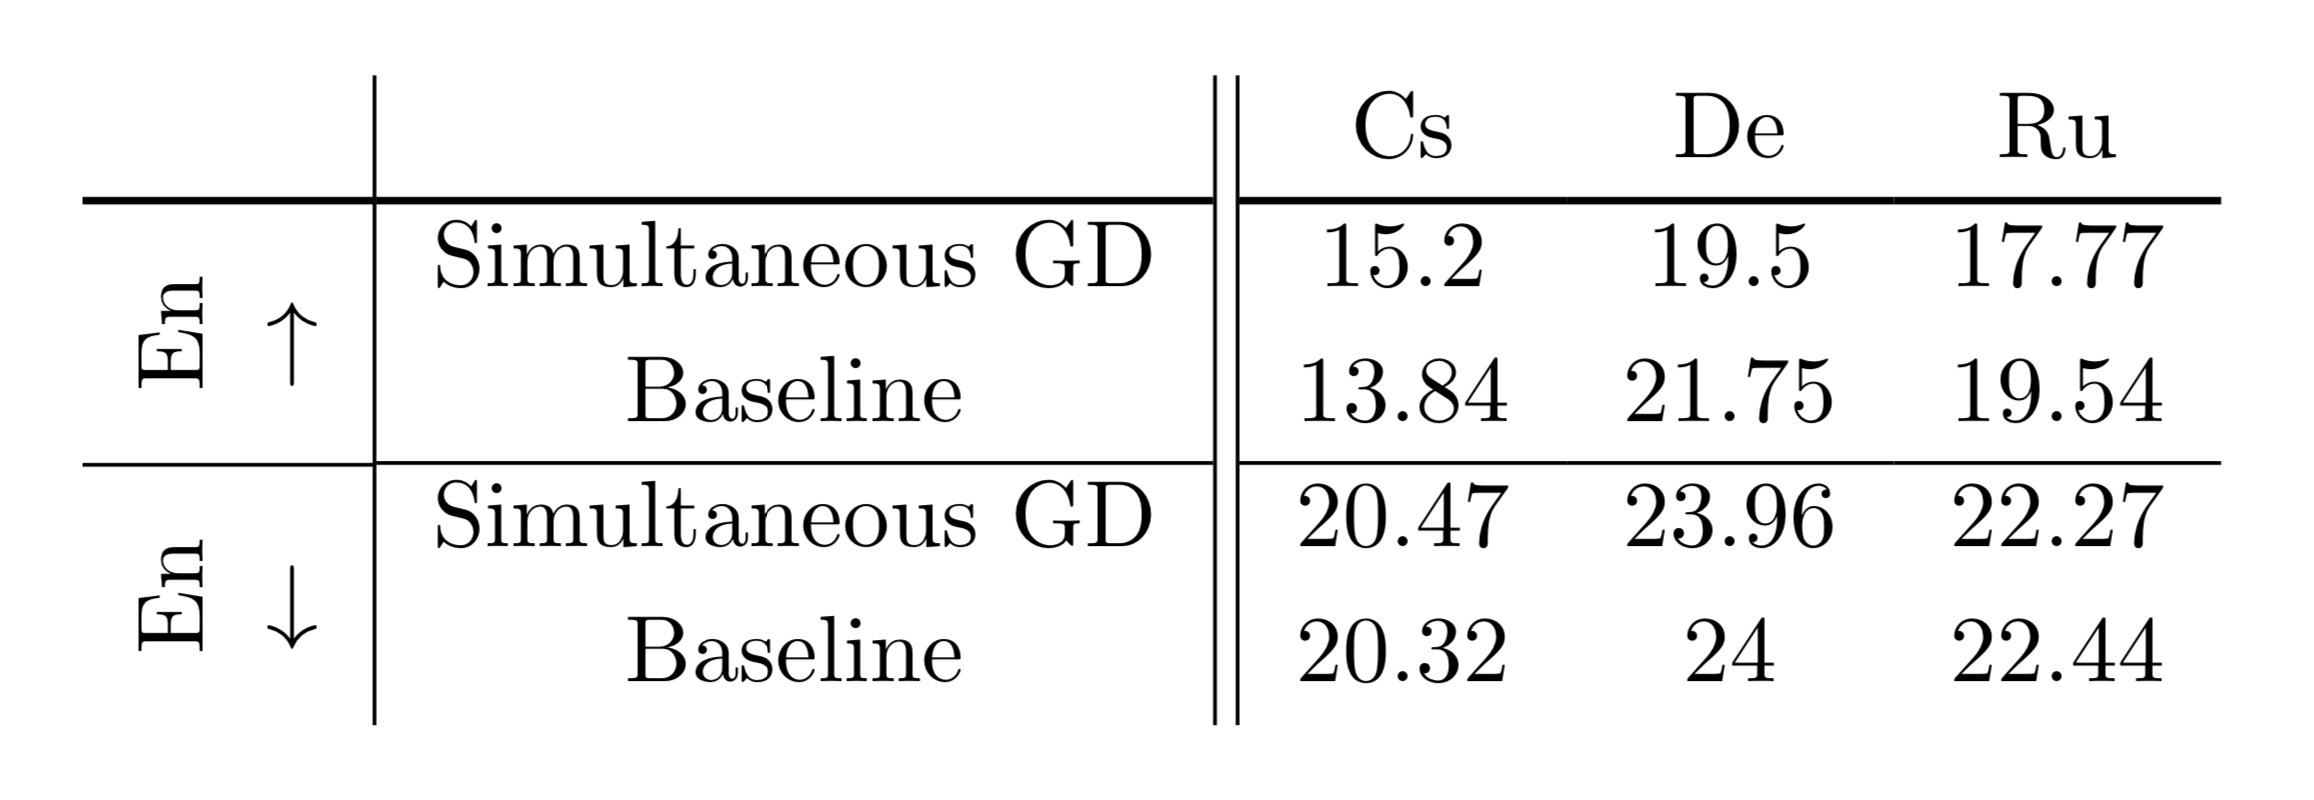
\includegraphics[scale=0.25]{./images/BLEU1}
%\caption{BLEU scores on the test set (newstest-2015) obtained by the models used in the paper and Baseline from (Firat et al., 2016). Although our models use a unidirectional recurrent net as an encoder, the translation qualities are comparable.}
%\end{figure}
%}

\frame{
\textbf{Results}\\
\vspace{1cm}
\begin{table}[h]
\centering
\begin{tabular}{|c|c|c|c|}
\hline
  \multicolumn{2}{|c|}{ }   & AP & BLEU  \\ \Xhline{2\arrayrulewidth}
\multirow{ 3}{*}{EN $\rightarrow$ DE} & WIW & 0.9  & 16  \\
                                      & WID & 0.79 & 15.6 \\
                                      & NMT & 1    & 19.5 \\ \Xhline{2\arrayrulewidth}
\multirow{ 3}{*}{DE $\rightarrow$ EN} & WIW & 0.9  & 17  \\
                                      & WID & 0.72 & 18  \\
                                      & NMT & 1    & 23.9 \\\hline
\end{tabular}
\label{table2}
\vspace{0.5cm}
\caption{WIW : Wait-If-Worse, WID : Wait-If-Diff, AP : Average Proportion.}
\end{table}

}

\frame{
\textbf{Discussion}
\begin{enumerate}
\item They do not have good BLEU score compared to previous works.
\item The waiting criteria proposed in this paper are both manually designed and does not exploit rich information embedded in the hidden representation learned by the recurrent neural networks.
\item The objective of the network is to improve translation quality and do not consider delay during training.
\end{enumerate}
}

\frame{
\textbf{Trainable Agent}
\begin{itemize}
\item The idea is to have a separate trainable agent
\item The framework can be trained using reinforcement learning and it considers both Quality and Delay during training.
\end{itemize}
\begin{figure}[!b]
\centering
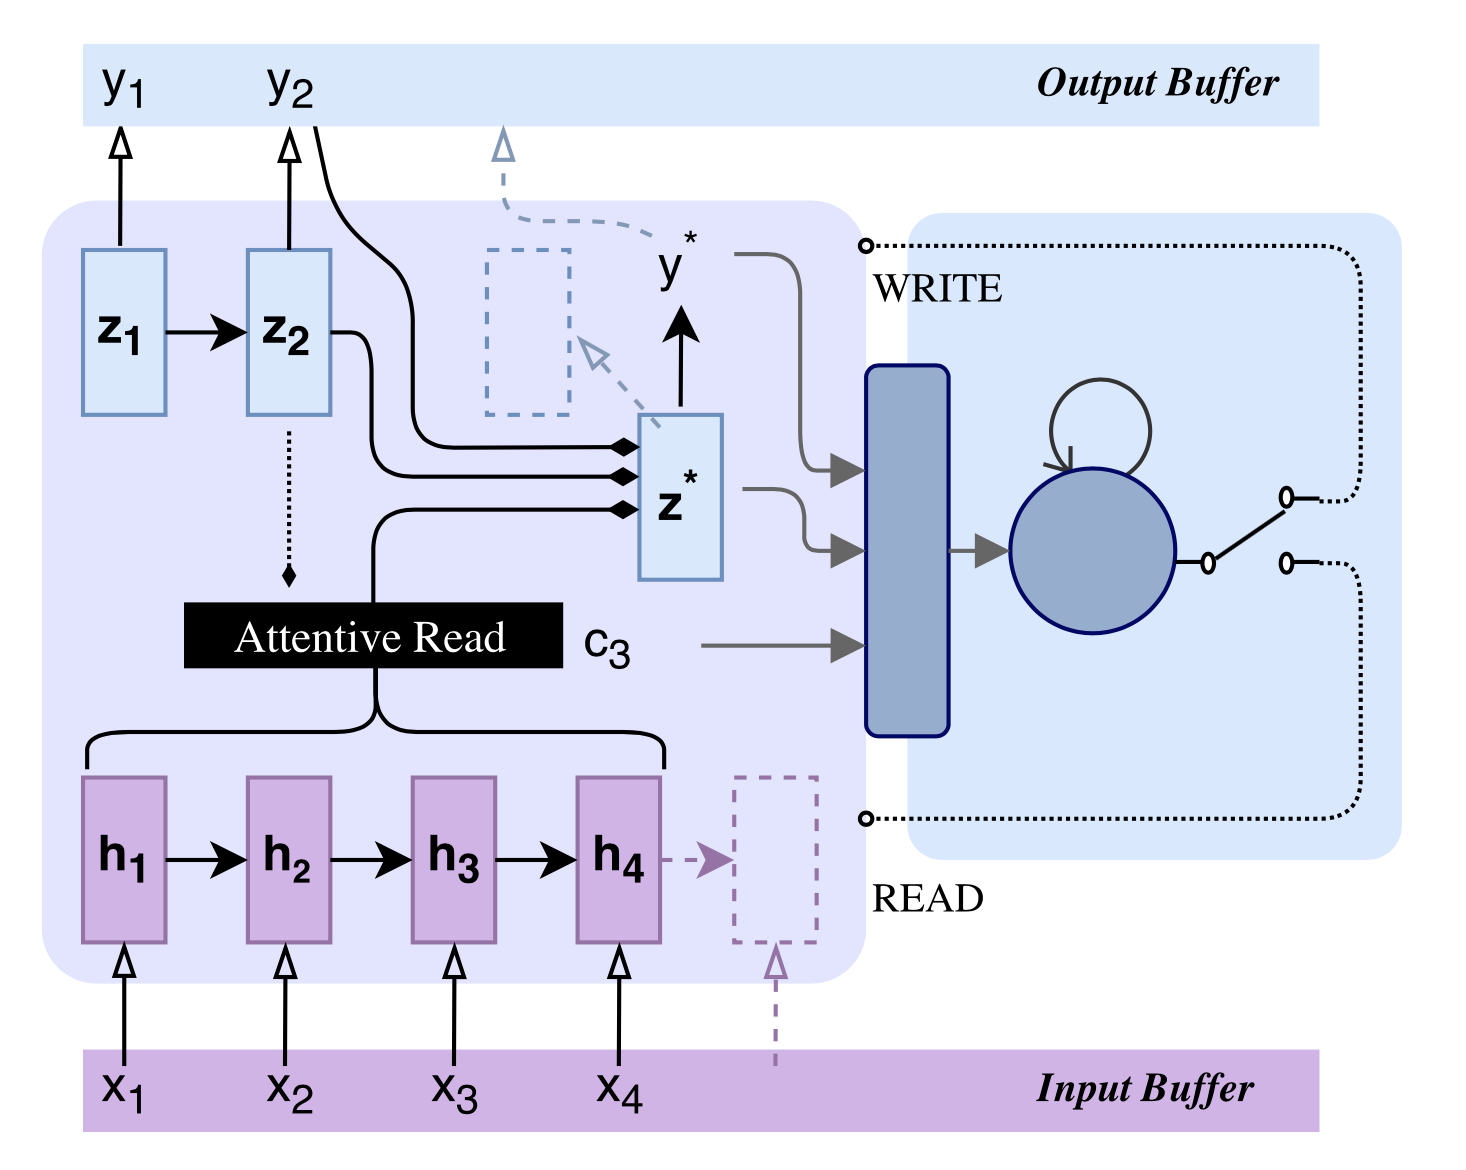
\includegraphics[scale=0.20]{./images/TA} \\[-1ex]
{\tiny Source: Gu et al. \cite{gu:2017:EACL}}
\end{figure}
}

\subsubsection[Q-network]{- Q-network}

\frame{
\textbf{Q-network agent } \hfill [Satija et al., 2016]\\
%\vspace{0.5cm}
\begin{figure}[h]
\centering
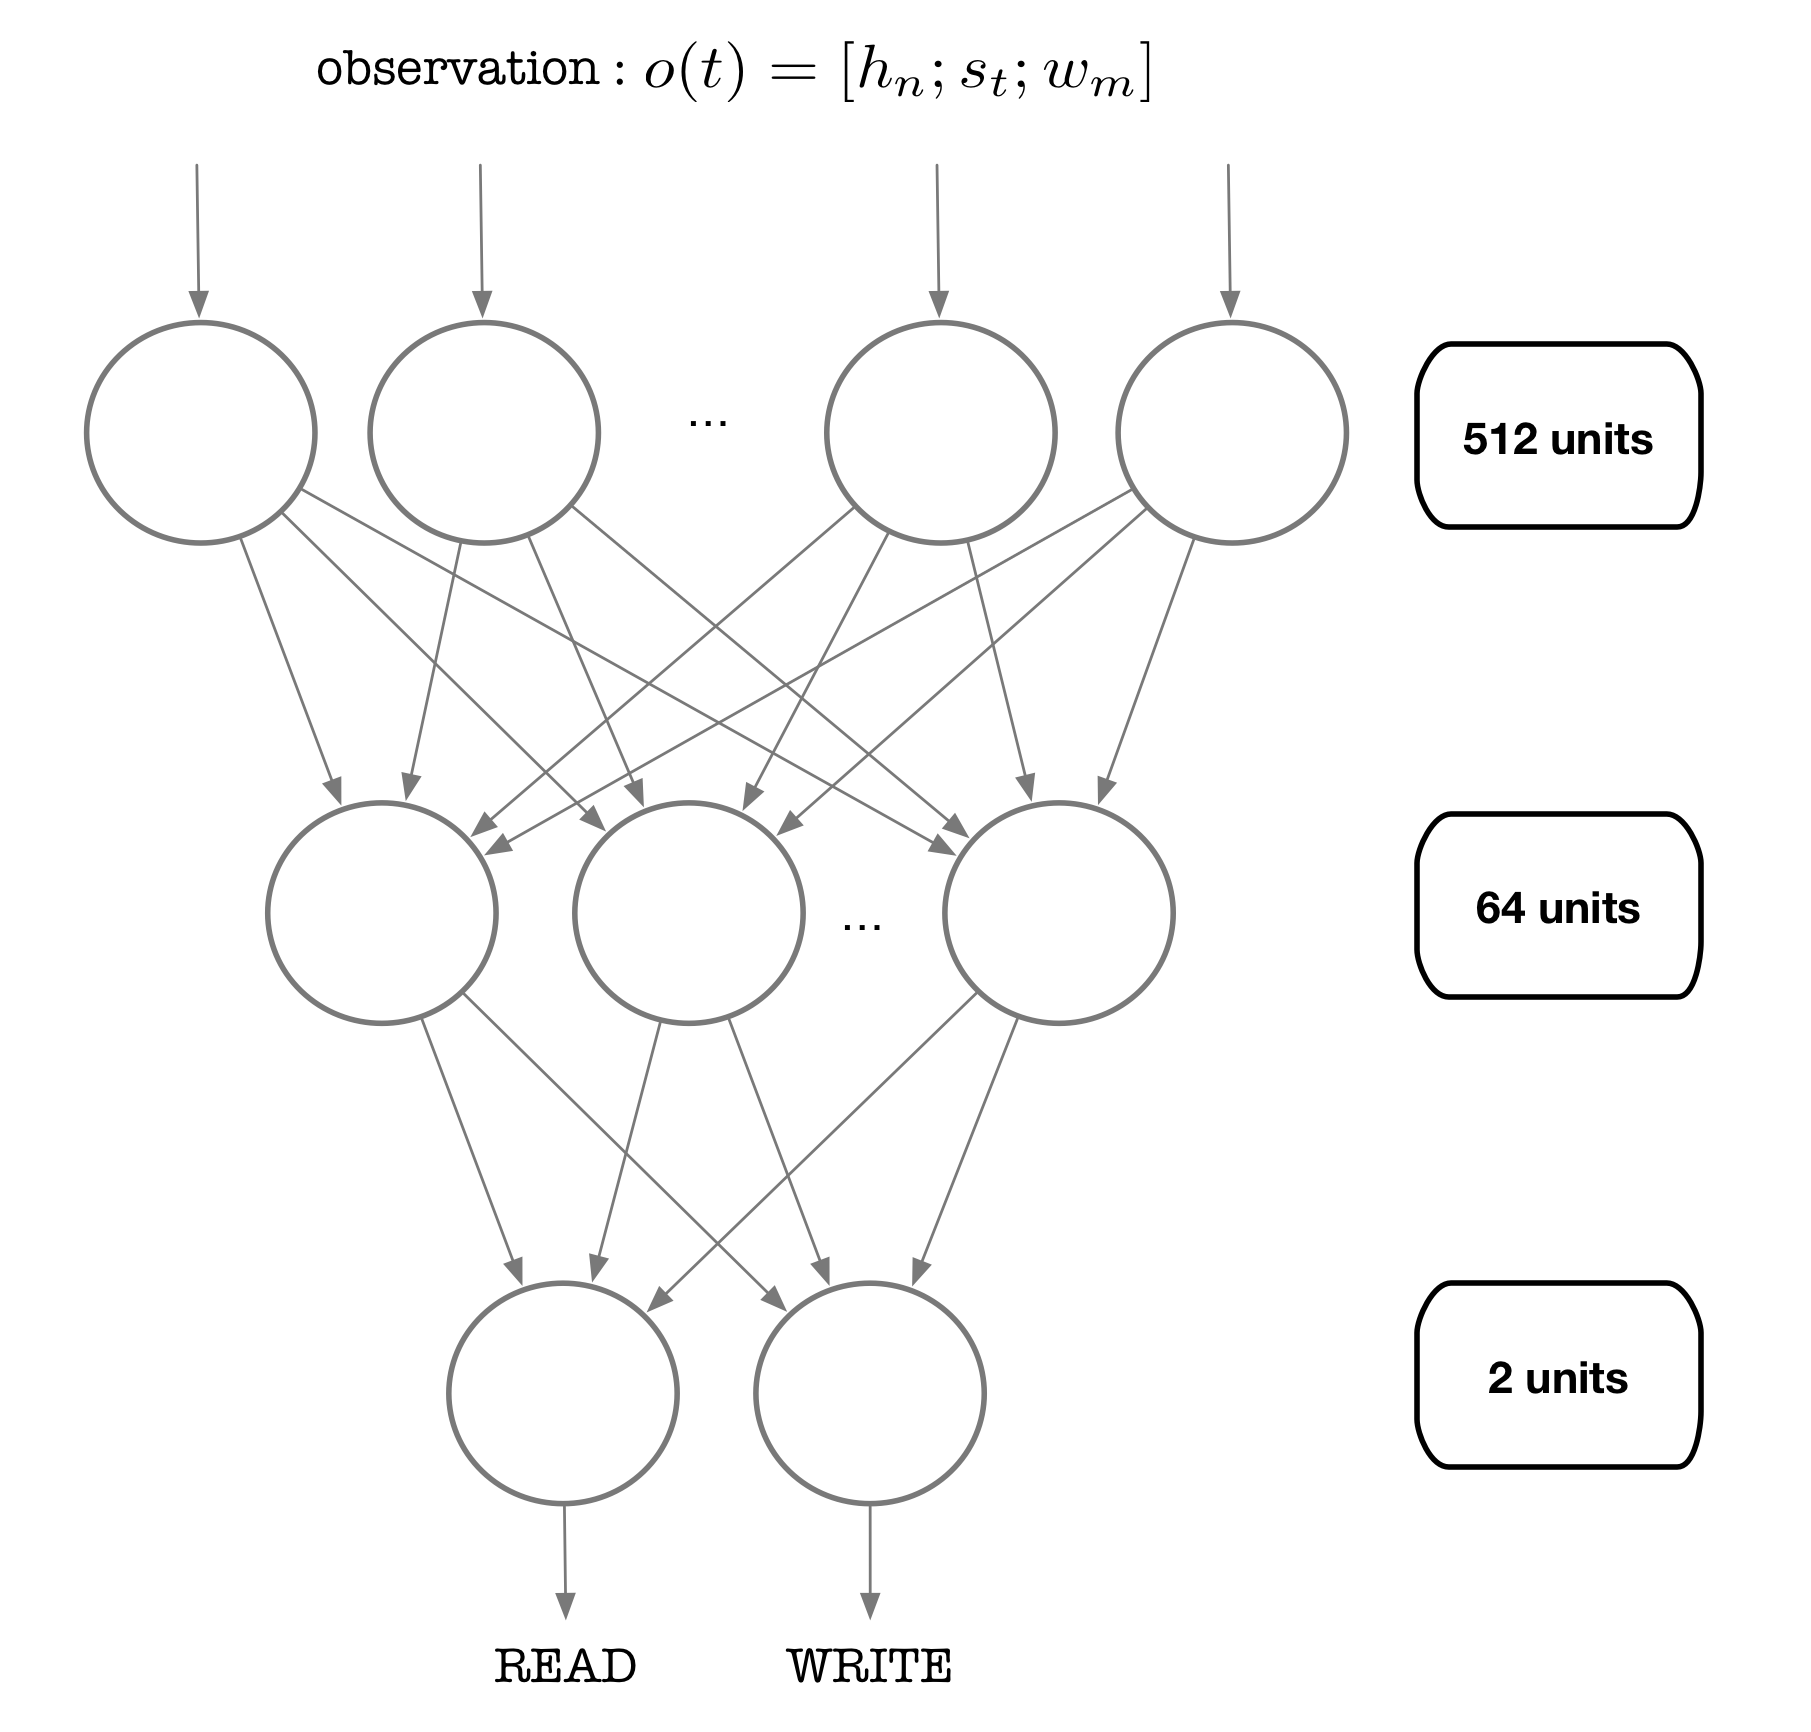
\includegraphics[scale=0.3]{./images/QNagent}
%\caption{Delay vs Translation quality (BLEU) for EN-FR and EN-DE language pairs.}
\end{figure}
}

\frame{
\textbf{Reward function}
\begin{itemize}
    \item \textbf{Quality} \\
    \begin{align*}
        r_t^Q = 
        \begin{cases}
        \frac{1}{\beta}\text{BLEU}(Y^t, Y^*) &  t<T\\
        \text{BLEU}(Y, Y^*)                  &  t=T
        \end{cases}
    \end{align*}
    \item \textbf{Delay}\\
    \begin{itemize}
        \item[-] $r_t^D$ = Wait Delay
    \end{itemize}
    
\end{itemize}
\vspace{1cm}
Total reward function is computed as:
$$r_t = r_t^Q \times r_t^D$$
}

\frame{
\textbf{Results}\\
%\vspace{0.5cm}
\begin{figure}[h]
\centering
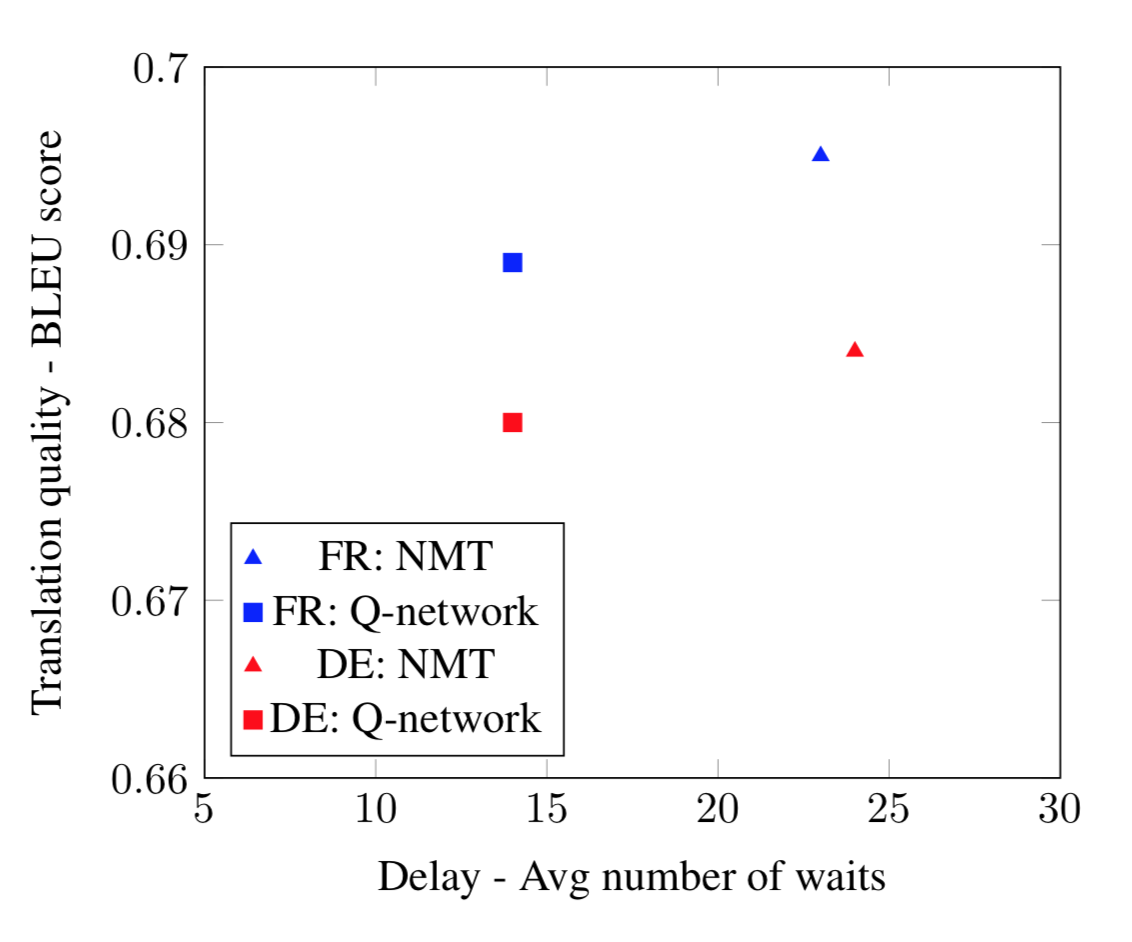
\includegraphics[scale=0.3]{./images/Qnetwork}
\caption{Delay vs Translation quality (BLEU) for EN-FR and EN-DE language pairs.}
\end{figure}
}

\subsubsection[Policy Gradient]{- Policy Gradient}


%\frame{
%\centering
%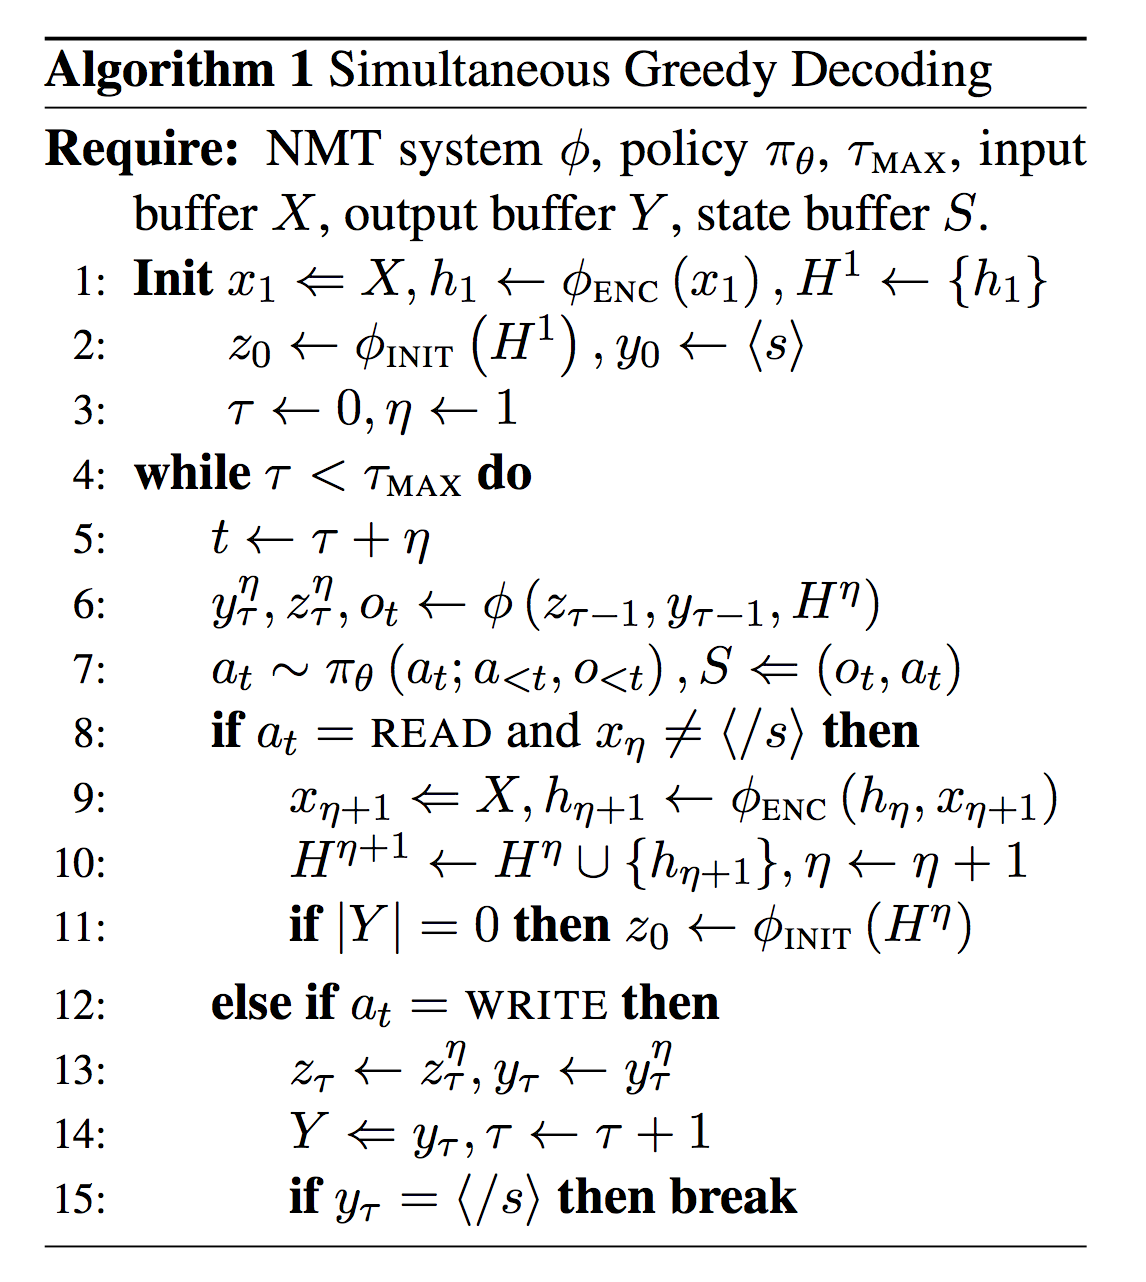
\includegraphics[scale=0.33]{./images/SGD}
%}

\frame{
\textbf{Policy gradient agent} \hfill [Gu et al., 2017]\\
%\vspace{0.5cm}
\begin{figure}[h]
\centering
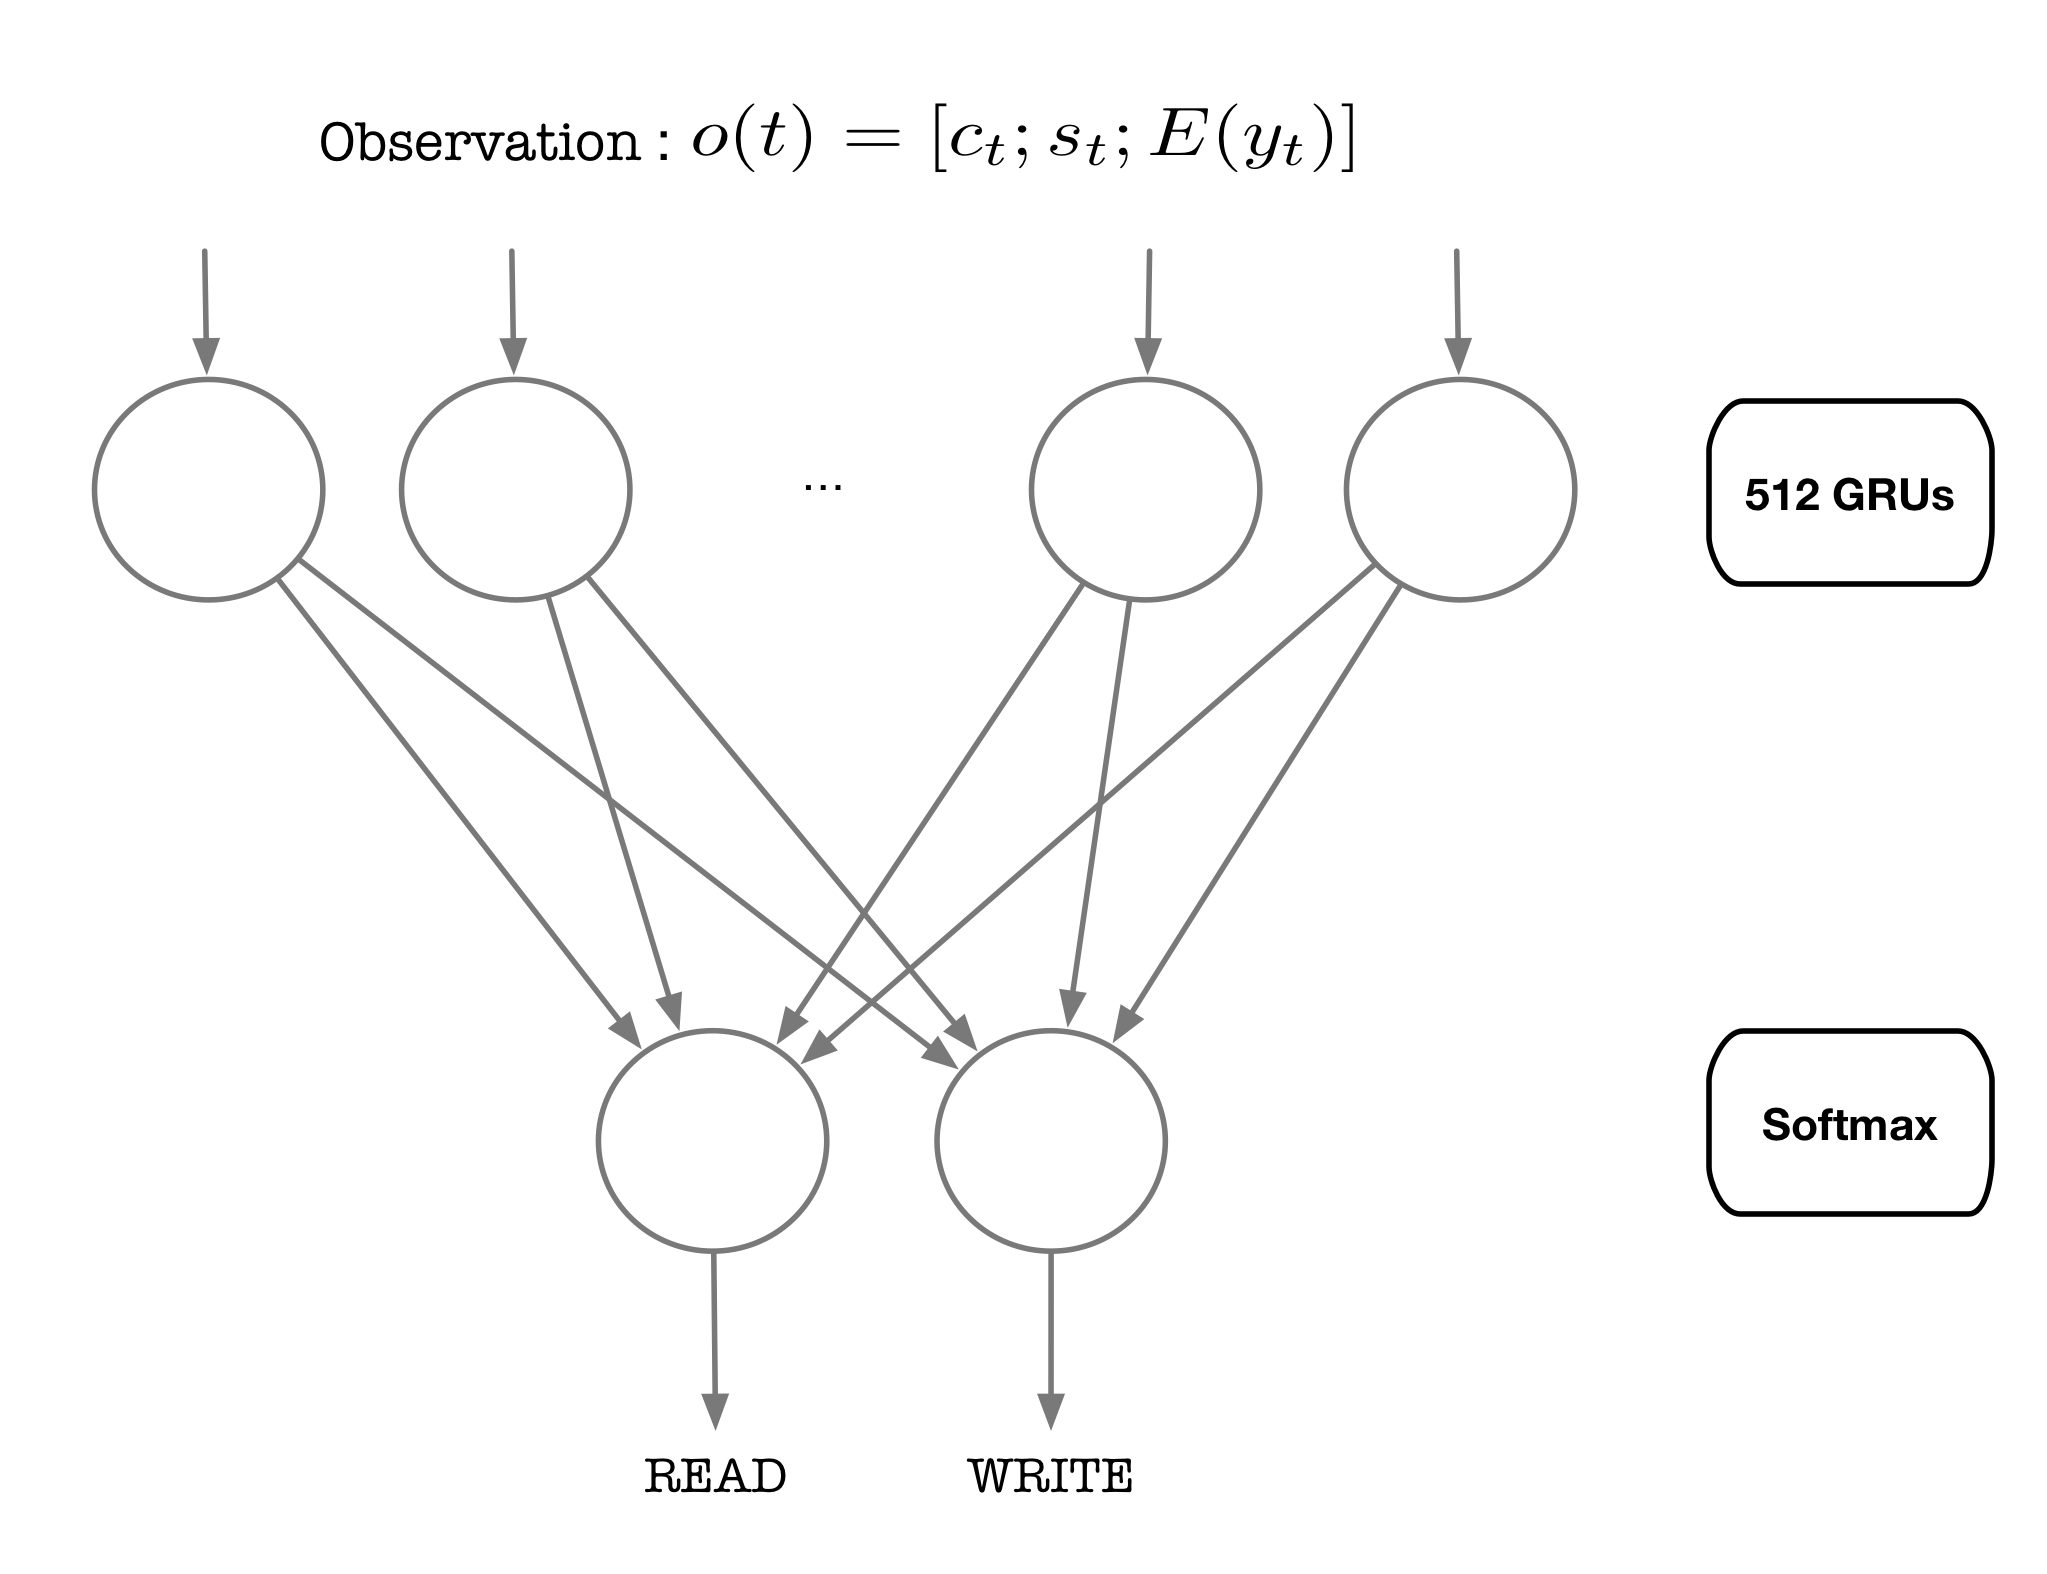
\includegraphics[scale=0.25]{./images/PGagent}
%\caption{Delay vs Translation quality (BLEU) for EN-FR and EN-DE language pairs.}
\end{figure}
}

%\frame{
%\textbf{Agent} \\
%A trainable agent is designed to make decisions $A = \{a_1, \dots, a_T \}$, $a_t \in \mathcal{A}$ sequentially based on observations $O = \{o_1, \dots, o_T \}$, $o_t \in \mathcal{O}$.\\
%\begin{itemize}
%\item \textbf{Observation: }  $o_{\tau + \eta} = [c_{\tau}^{\eta};z_{\tau}^{\eta};E(y_{\tau}^{\eta})]$
%\item \textbf{Action: }
%\begin{itemize}
%\item READ: waits to encode the next word
%\item WRITE: accepts the candidate and emits it as the prediction
%\end{itemize}
%\item \textbf{Policy: } a stochastic policy $\pi_{\theta}$ parameterized by a recurrent neural network
%\begin{equation*}
%\centering
%\begin{aligned}
%&s_t = f_\theta (s_{t-1}, o_t),  \\
%&\pi_\theta (a_t | a_{<t}, o_{\leq t} ) \propto g_\theta (s_t)
%\end{aligned}
%\end{equation*}
%\end{itemize}
%}

\frame{
\textbf{Reward Function} \\
At each step the agent will receive a reward signal $r_t$ based on ($o_t$, $a_t$).
\begin{itemize}
\item \textbf{Quality $ r_t^Q $}
= smoothed BLEU
\item \textbf{Delay $ r_t^D $}
\begin{enumerate}
\item \textbf{Average Proportion}
\item \textbf{Consecutive Wait Length}
\end{enumerate}
\end{itemize}

The total reward will be computed as:
$$r_t = r_t^Q + r_t^D$$
}

\frame{
\textbf{Results for Policy Grdient:}\\
%\vspace{0.7cm}
\begin{table}
\centering
 \begin{tabular}{| c | c || c | c | } 
 \hline
 \multicolumn{2}{|c||}{ } & AP & BLEU \\ [0.5ex] 
 \Xhline{2\arrayrulewidth}
 \multirow{ 2}{*}{EN $\rightarrow$ DE} & PG  & 0.8 & 17   \\
                                       & NMT & 1   & 19.5 \\ \Xhline{2\arrayrulewidth}
 \multirow{ 2}{*}{DE $\rightarrow$ EN} & PG  & 0.79 & 21.9 \\ 
                                       & NMT & 1    & 23.9 \\ \hline
\end{tabular}
\label{tab:Final}
\end{table}

\vspace{0.5cm}
\semitransp[40]{
Results for Greedy Decoding: 
\begin{table}[h]
\centering
\begin{tabular}{|c|c|c|c|}
\hline
  \multicolumn{2}{|c|}{ }   & AP & BLEU  \\ \Xhline{2\arrayrulewidth}
\multirow{ 3}{*}{EN $\rightarrow$ DE} & WIW & 0.9  & 16  \\
                                      & WID & 0.79 & 15.6 \\
                                      & NMT & 1    & 19.5 \\ \Xhline{2\arrayrulewidth}
\multirow{ 3}{*}{DE $\rightarrow$ EN} & WIW & 0.9  & 17  \\
                                      & WID & 0.72 & 18  \\
                                      & NMT & 1    & 23.9 \\\hline
\end{tabular}
\label{table2}
\end{table}
}
}

%\frame{
%\centering
%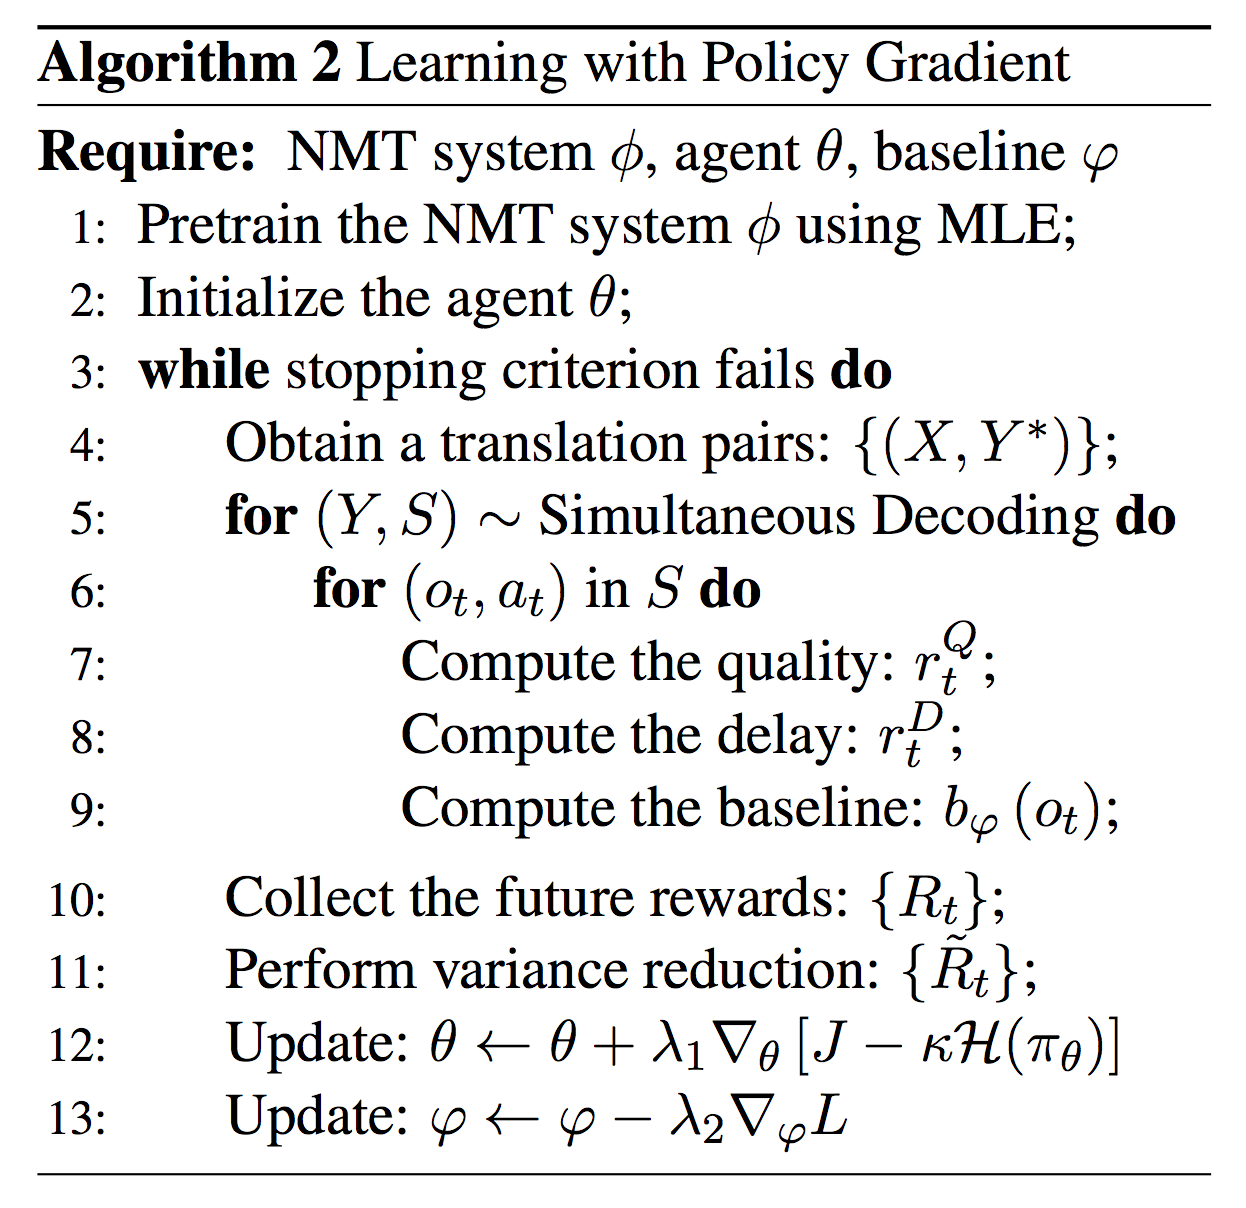
\includegraphics[scale=0.33]{./images/PG}
%}

%\frame{
%\textbf{Results}
%\vspace{1cm}

%\begin{columns}
%\column{0.5\textwidth}
%\centering
%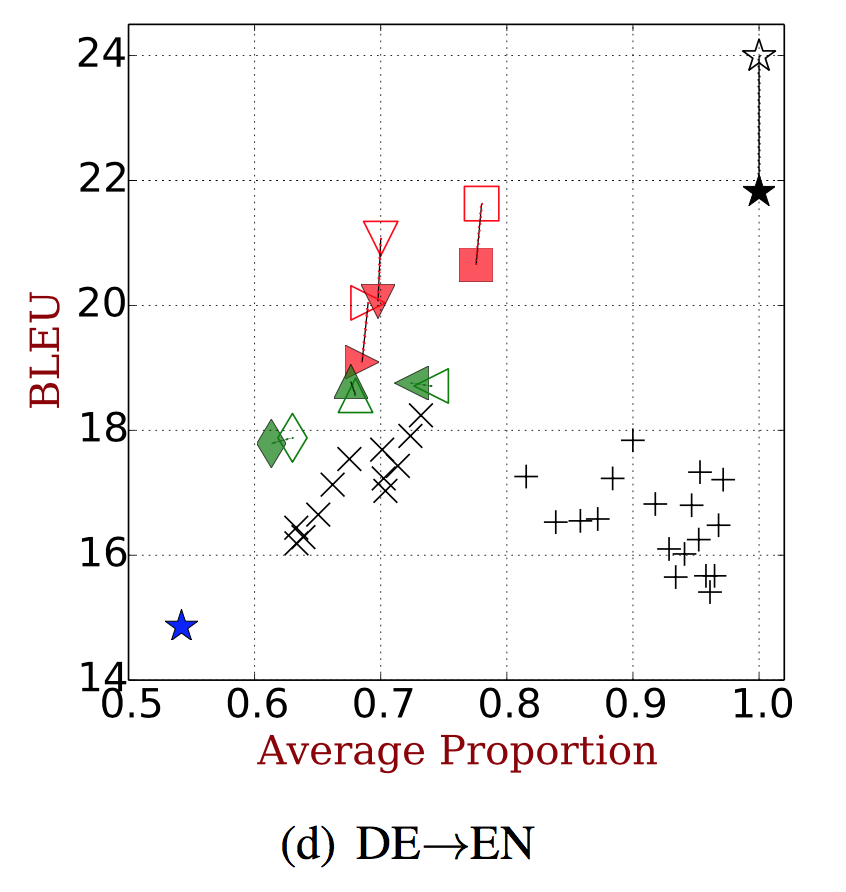
\includegraphics[scale=0.28]{./images/DEEN}
%\column{0.5\textwidth}
%\centering
%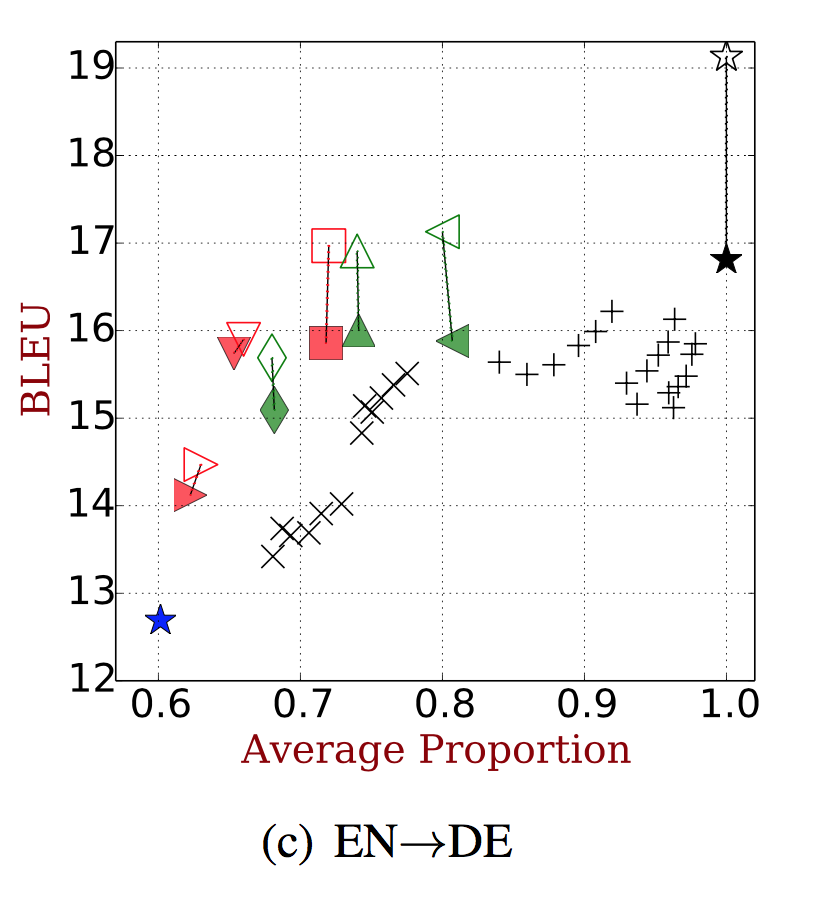
\includegraphics[scale=0.28]{./images/ENDE}
%\end{columns}

%\vspace{1cm}
%\centering
%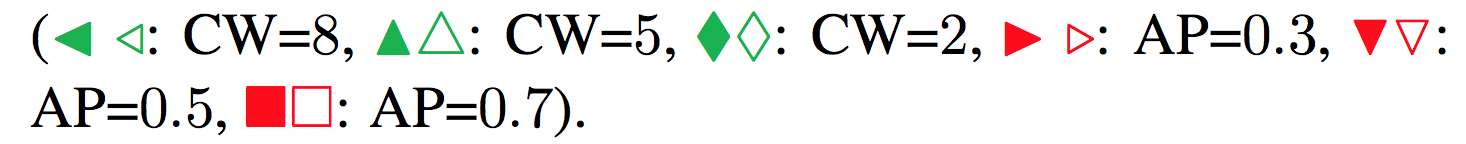
\includegraphics[scale=0.3]{./images/GUIDE}

%}

\frame{
\textbf{Discussion}
\begin{enumerate}
\item We have full control over balancing the trade-off between Quality and Delay.
\item Still not very good scores on quality of translation 
\item Cannot perform well on translating from SVO languages like EN to SOV languages like DE.
\end{enumerate}
}

\frame{
\textbf{Future Direction}
\begin{itemize}
    \item We are not sure if it's the best way for SNMT.
    \item Lots of solved problems from statistical approaches are still unsolved in this framework:
    \begin{itemize}
        \item Paraphrasing
        \item Prediction
        \item ...
    \end{itemize}
    \item Applying ensembles are still challenging in this field. 
\end{itemize}
}
%===================================================================================

%\section{prediction}
%\frame{
%\begin{center}
%\Huge Prediction
%\end{center}
%}

%\subsection{Importance of prediction}
%\frame{
%\frametitle{Importance of prediction}
%\begin{itemize}
%    \item Translation in real-time from Subject-Object-Verb (SOV) languages like Germany to Subject-Verb-Object (SVO) languages like English would be impossible without prediction.
%\end{itemize}
%\vfill
%\centering
%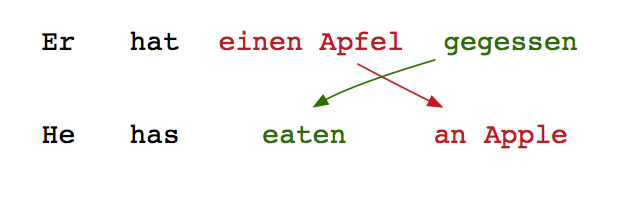
\includegraphics[scale=0.3]{./images/SOV-SVO}
%}

%\subsection{Our Idea}
%\frame{
%\frametitle{Our Method}
%\textbf{Our Method}
%\begin{itemize}
%    \item Our idea is to have another action called "Predict".
%    \item It will predict one word at a time.
%    \item If the agent chooses "predict", then our predictor will generate a word as input.
%    \item Our predictor is a pre-trained multi-layer LSTM network for word-level language models.
%\end{itemize}
%}

%\frame{
%\textbf{Structure of the Network}
%\centering
%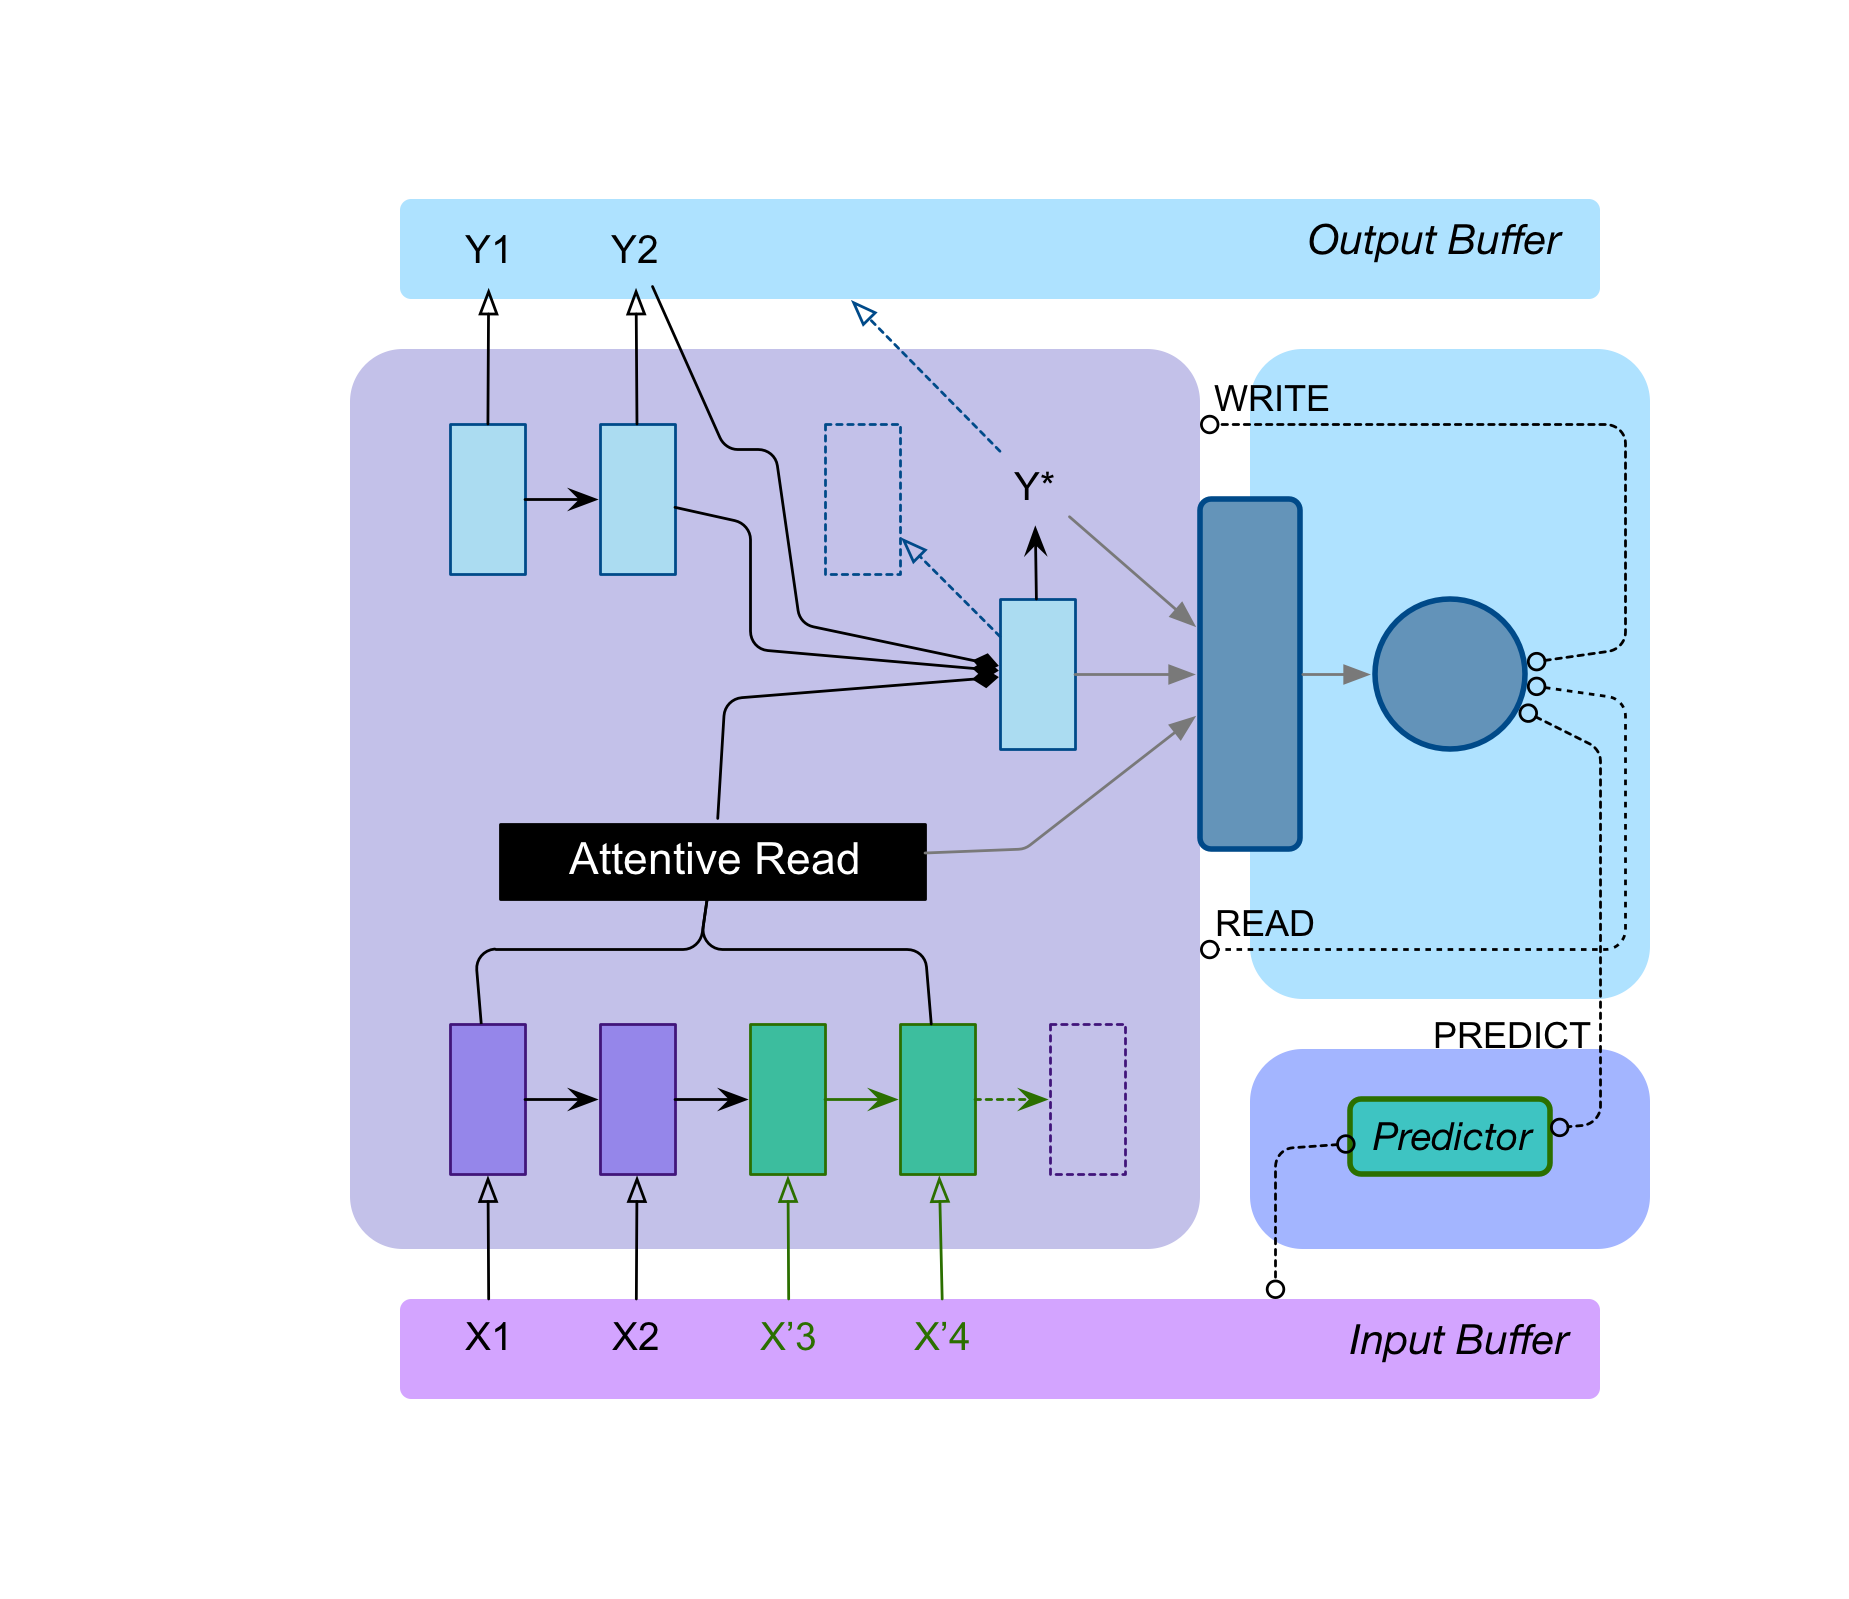
\includegraphics[scale=0.36]{./images/Predicted.png}
%}


%===================================================================================
\section*{}

%\begin{frame}
%\textbf{References in here}
%\end{frame}

\begin{frame}
\textbf{References}
\vspace{5mm}
\nocite{*}
\bibliographystyle{unsrt}
\footnotesize
\bibliography{Reference}
\end{frame}

\begin{frame}
\only<1>{
\begin{center}
\Huge Thank You !

\end{center}
}

\only<2>{
\begin{center}
    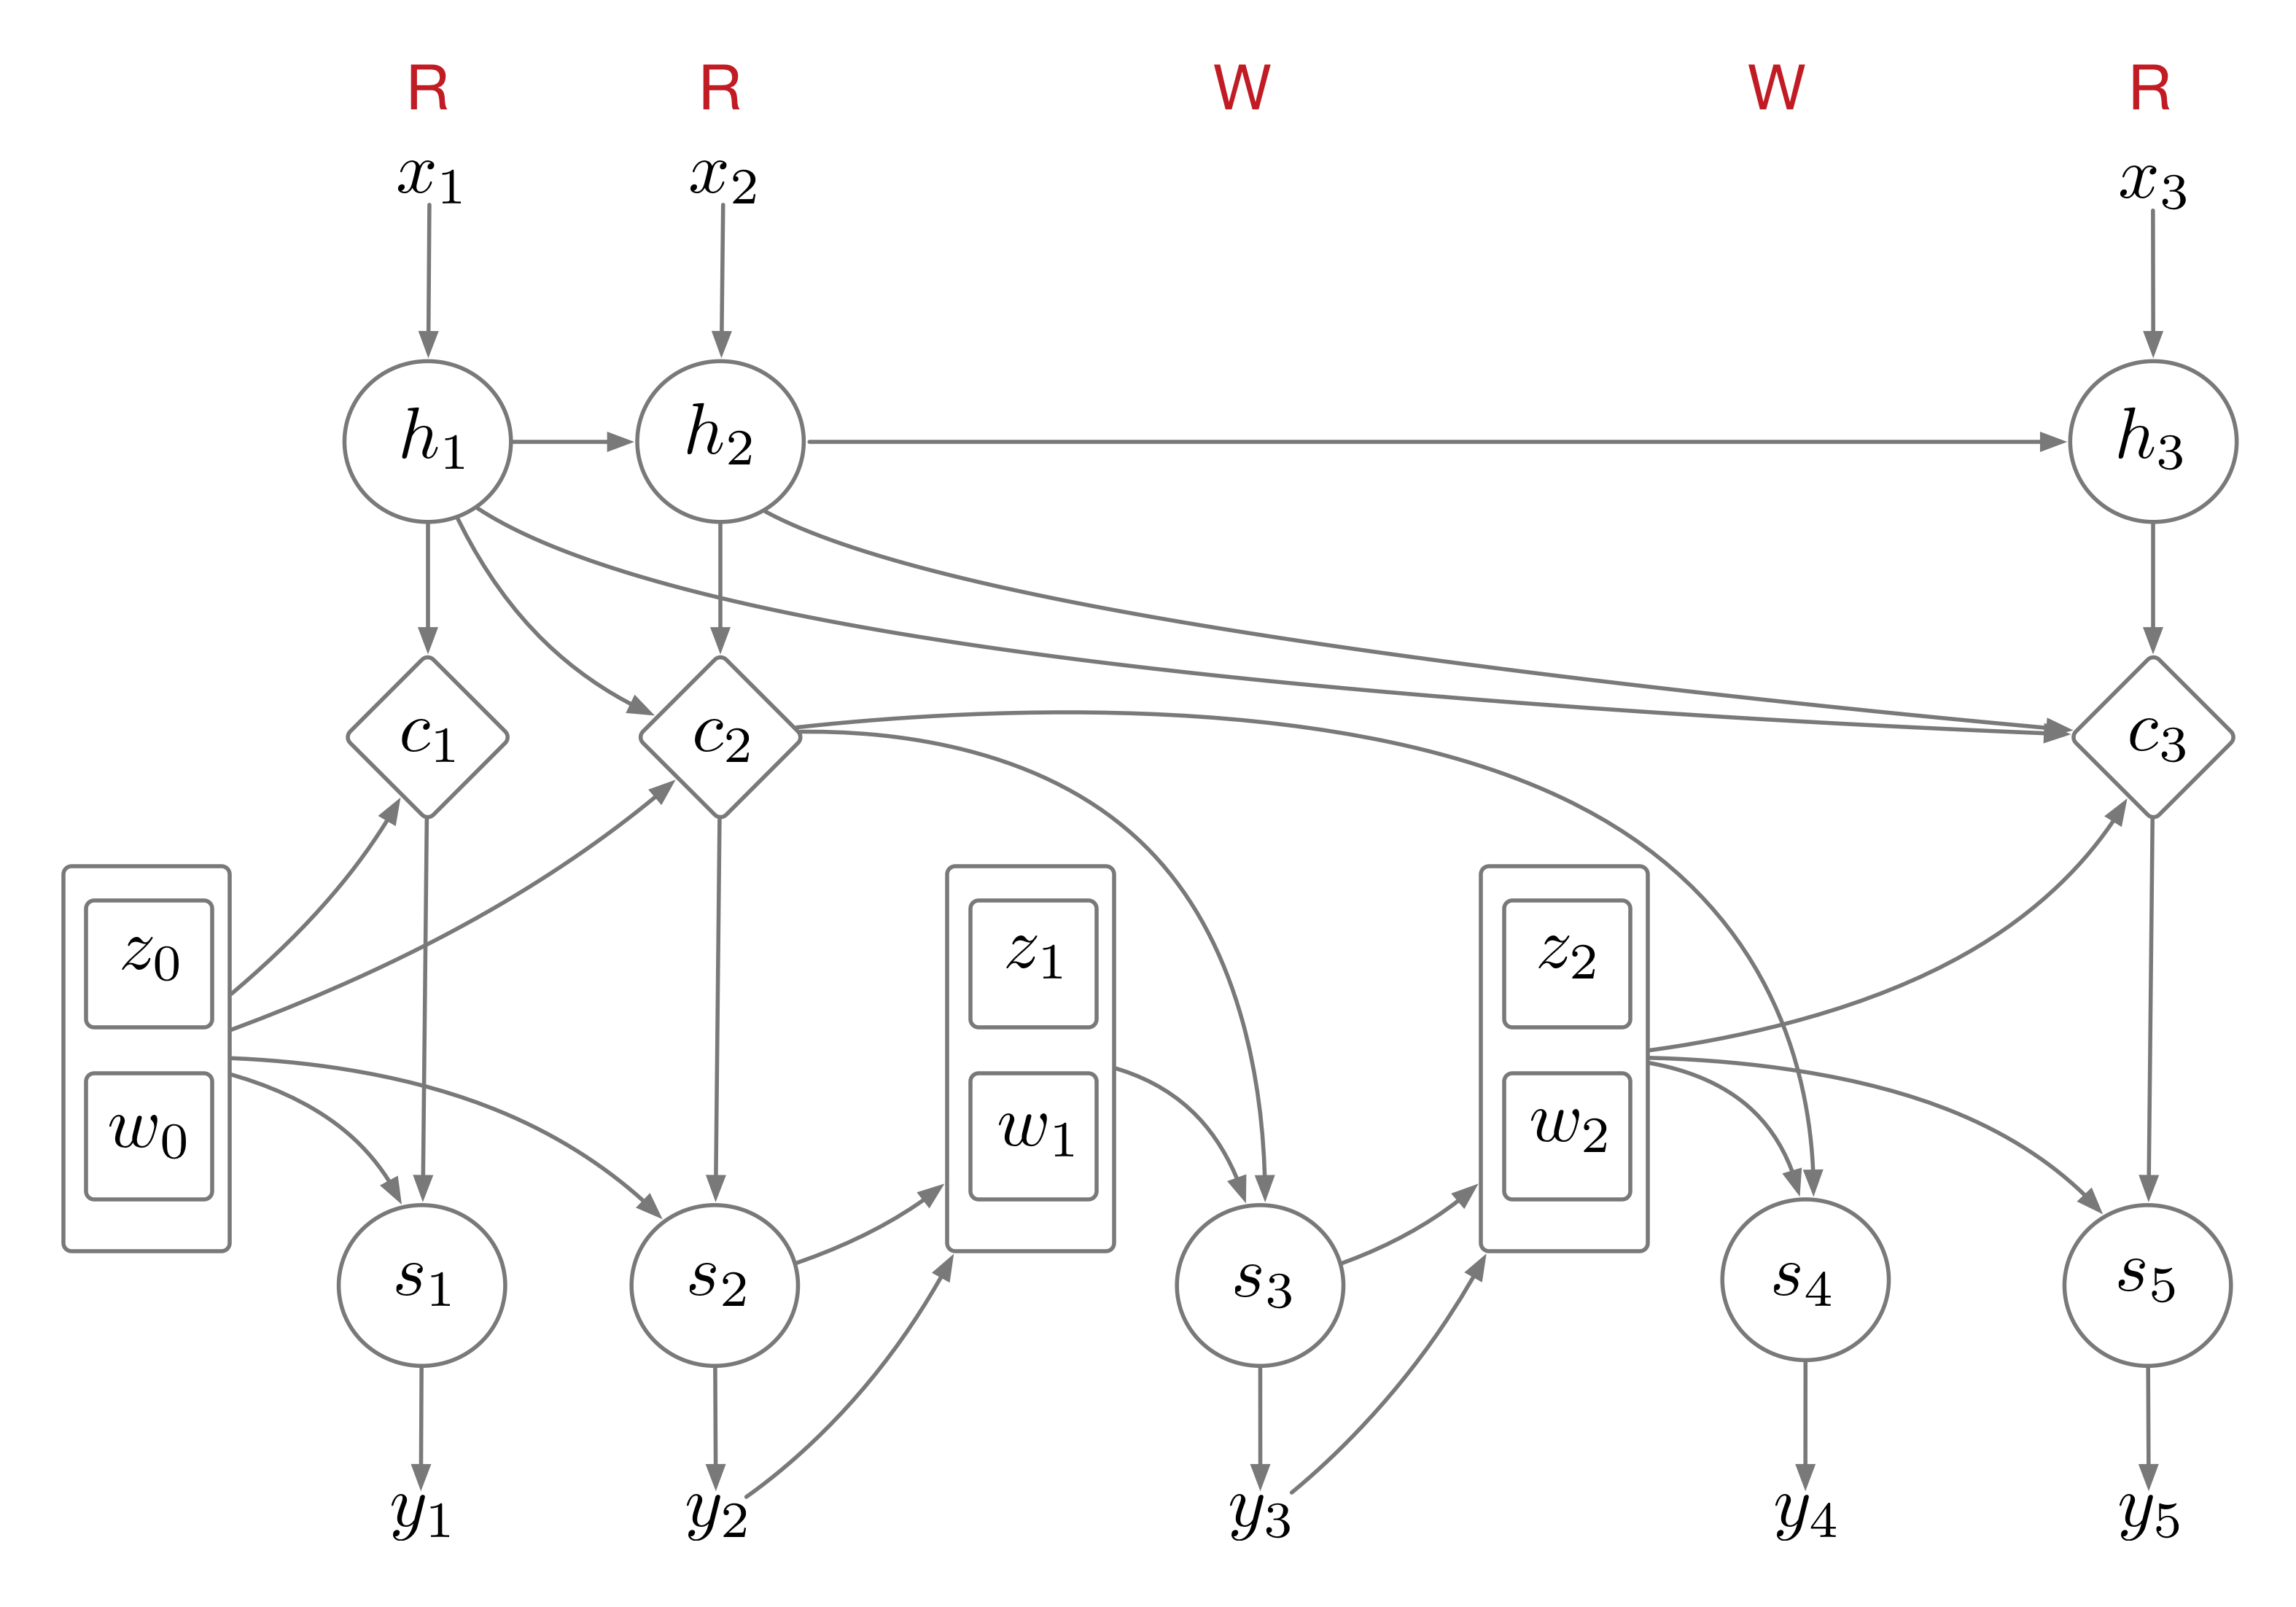
\includegraphics[scale=0.20]{./images/complete}
\end{center}
}

\only<3>{
\textbf{LSTM}:
\begin{center}
    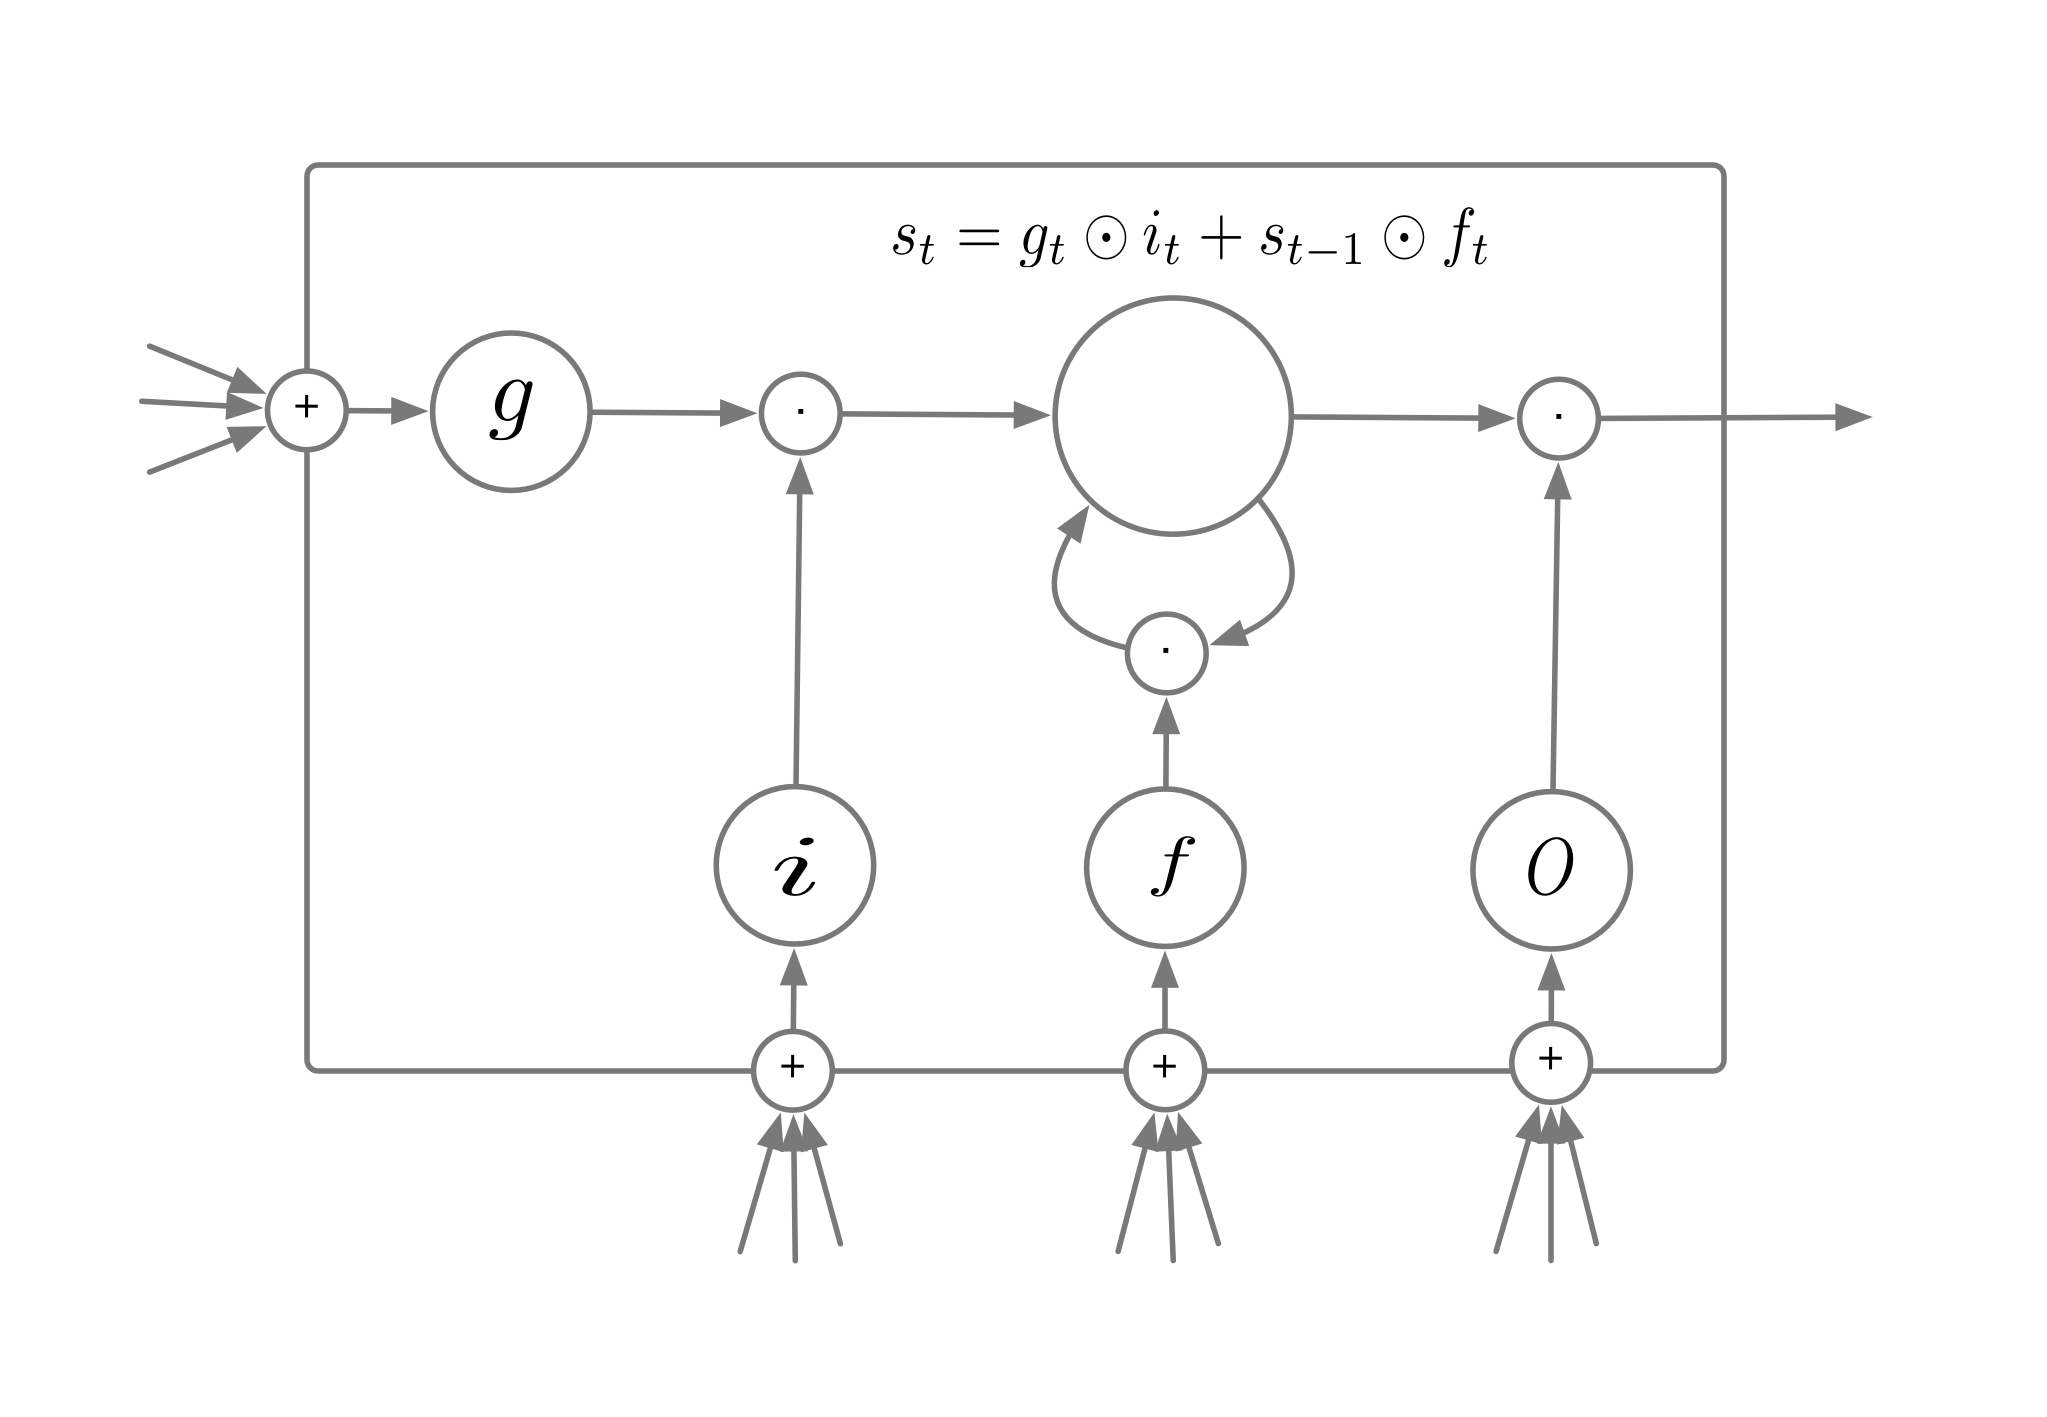
\includegraphics[scale=0.080]{./images/LSTM}
\end{center}
\vspace{-0.5cm}
\begin{align*}
\centering
&g_t = \phi (W_{gx}x_t + W_{gh}h_{t-1} + b_g) \label{eq:1.1}\\
&i_t = \sigma (W_{ix}x_t + W_{ih}h_{t-1} + b_i) \label{eq:1.2}\\
&f_t = \sigma (W_{fx}x_t + W_{fh}h_{t-1} + b_f) \label{eq:1.3}\\
&o_t = \sigma (W_{ox}x_t + W_{oh}h_{t-1} + b_o) \label{eq:1.4}\\ 
&s_t = g_t \odot i_i + s_{t-1} \odot f_t \label{eq:1.5}\\
&h_t = \phi(s_t) \odot o_t
\end{align*}

}
\end{frame}

%===================================================================================
%\frame{
%\frametitle{Sample Frame Title No. 3}
%Lorem ipsum dolor sit amet, consectetur adipiscing elit, sed do eiusmod tempor incididunt ut labore et dolore magna aliqua. 
%\begin{block}{Something important}
%Einstein's formula
%$$E=mc^2$$
%\end{block}
%}

%\frame{
%\frametitle{Sample Frame Title No. 2}
%\begin{itemize}
%\item First item
%\item Second item
%\item Third item
%\end{itemize}
%}

%\frametitle{Sample Frame Title No. 1}
%Lorem ipsum dolor sit amet, consectetur adipiscing elit, sed do eiusmod tempor incididunt ut labore et dolore magna aliqua. Ut enim ad minim veniam, quis nostrud exercitation ullamco laboris nisi ut aliquip ex ea commodo consequat. Duis aute irure dolor in reprehenderit in voluptate velit esse cillum dolore eu fugiat nulla pariatur. Excepteur sint occaecat cupidatat non proident, sunt in culpa qui officia deserunt mollit anim id est laborum.
%}

%\subsection{Sample subsection}


\end{document}
